\documentclass[floatsintext,man]{apa6}

\usepackage{amssymb,amsmath}
\usepackage{ifxetex,ifluatex}
\usepackage{fixltx2e} % provides \textsubscript
\ifnum 0\ifxetex 1\fi\ifluatex 1\fi=0 % if pdftex
  \usepackage[T1]{fontenc}
  \usepackage[utf8]{inputenc}
\else % if luatex or xelatex
  \ifxetex
    \usepackage{mathspec}
    \usepackage{xltxtra,xunicode}
  \else
    \usepackage{fontspec}
  \fi
  \defaultfontfeatures{Mapping=tex-text,Scale=MatchLowercase}
  \newcommand{\euro}{€}
\fi
% use upquote if available, for straight quotes in verbatim environments
\IfFileExists{upquote.sty}{\usepackage{upquote}}{}
% use microtype if available
\IfFileExists{microtype.sty}{\usepackage{microtype}}{}

% Table formatting
\usepackage{longtable, booktabs}
\usepackage{lscape}
% \usepackage[counterclockwise]{rotating}   % Landscape page setup for large tables
\usepackage{multirow}		% Table styling
\usepackage{tabularx}		% Control Column width
\usepackage[flushleft]{threeparttable}	% Allows for three part tables with a specified notes section
\usepackage{threeparttablex}            % Lets threeparttable work with longtable

% Create new environments so endfloat can handle them
% \newenvironment{ltable}
%   {\begin{landscape}\begin{center}\begin{threeparttable}}
%   {\end{threeparttable}\end{center}\end{landscape}}

\newenvironment{lltable}
  {\begin{landscape}\begin{center}\begin{ThreePartTable}}
  {\end{ThreePartTable}\end{center}\end{landscape}}




% The following enables adjusting longtable caption width to table width
% Solution found at http://golatex.de/longtable-mit-caption-so-breit-wie-die-tabelle-t15767.html
\makeatletter
\newcommand\LastLTentrywidth{1em}
\newlength\longtablewidth
\setlength{\longtablewidth}{1in}
\newcommand\getlongtablewidth{%
 \begingroup
  \ifcsname LT@\roman{LT@tables}\endcsname
  \global\longtablewidth=0pt
  \renewcommand\LT@entry[2]{\global\advance\longtablewidth by ##2\relax\gdef\LastLTentrywidth{##2}}%
  \@nameuse{LT@\roman{LT@tables}}%
  \fi
\endgroup}


\ifxetex
  \usepackage[setpagesize=false, % page size defined by xetex
              unicode=false, % unicode breaks when used with xetex
              xetex]{hyperref}
\else
  \usepackage[unicode=true]{hyperref}
\fi
\hypersetup{breaklinks=true,
            pdfauthor={},
            pdftitle={Supplementary Materials: Early language experience in a Tseltal Mayan village},
            colorlinks=true,
            citecolor=blue,
            urlcolor=blue,
            linkcolor=black,
            pdfborder={0 0 0}}
\urlstyle{same}  % don't use monospace font for urls

\setlength{\parindent}{0pt}
%\setlength{\parskip}{0pt plus 0pt minus 0pt}

\setlength{\emergencystretch}{3em}  % prevent overfull lines


% Manuscript styling
\captionsetup{font=singlespacing,justification=justified}
\usepackage{csquotes}
\usepackage{upgreek}

 % Line numbering
  \usepackage{lineno}
  \linenumbers


\usepackage{tikz} % Variable definition to generate author note

% fix for \tightlist problem in pandoc 1.14
\providecommand{\tightlist}{%
  \setlength{\itemsep}{0pt}\setlength{\parskip}{0pt}}

% Essential manuscript parts
  \title{Supplementary Materials: Early language experience in a Tseltal Mayan
village}

  \shorttitle{Supp. Materials: Early language in a Tseltal village}


  \author{Marisa Casillas\textsuperscript{1}, Penelope Brown\textsuperscript{1}, \& Stephen C. Levinson\textsuperscript{1}}

  % \def\affdep{{"", "", ""}}%
  % \def\affcity{{"", "", ""}}%

  \affiliation{
    \vspace{0.5cm}
          \textsuperscript{1} Max Planck Institute for Psycholinguistics  }

  \authornote{
    Correspondence concerning this article should be addressed to Marisa
    Casillas, P.O. Box 310, 6500 AH Nijmegen, The Netherlands. E-mail:
    \href{mailto:Marisa.Casillas@mpi.nl}{\nolinkurl{Marisa.Casillas@mpi.nl}}
  }


  



  \usepackage{float}
  \floatplacement{figure}{H}
  \usepackage{placeins}

\usepackage{amsthm}
\newtheorem{theorem}{Theorem}[section]
\newtheorem{lemma}{Lemma}[section]
\theoremstyle{definition}
\newtheorem{definition}{Definition}[section]
\newtheorem{corollary}{Corollary}[section]
\newtheorem{proposition}{Proposition}[section]
\theoremstyle{definition}
\newtheorem{example}{Example}[section]
\theoremstyle{definition}
\newtheorem{exercise}{Exercise}[section]
\theoremstyle{remark}
\newtheorem*{remark}{Remark}
\newtheorem*{solution}{Solution}
\begin{document}

\maketitle

\setcounter{secnumdepth}{0}



\section{Full model outputs}\label{models}

In the main text we only report \emph{significant} effects on the five
speech environment variables: TCDS min/hr, ODS min/hr, TC--O
transitions/min, O--TC transitions/min, and sequence duration. Here in
the Supplementary Materials we give the full model outputs for each
analysis, including re-leveled versions of each model to show all three
of the two-way tests between the three-level time-of-day factor. We also
show, for each of the five measures, a figure showing how the variable
is distributed across clips and a figure showing the distribution of
model residuals. We also include full model output and residuals for a
pair of comparably constructed gaussian mixed-effects regressions using
a logged dependent measure. A gaussian model with logged measures is a
more common solution to analyzing non-normal distributions in current
psycholinguistics, but is not suitable for the current data given how
our five speech environment measures are distributed, particularly in
the randomly sampled clips (see, e.g., Figures
\protect\hyperlink{fig1}{1}, \protect\hyperlink{fig7}{7},
\protect\hyperlink{fig10}{10}, \protect\hyperlink{fig13}{13},
\protect\hyperlink{fig19}{19}). Overall, however, the gaussian models
show a qualitatively similar pattern of results.

In what follows, the same information is shown for each of the five
speech environment measures. All models were run with the glmm-TMB
library in R (Brooks et al., 2017a, 2017b). Note that in all negative
binomial regressions, the dependent variables have been rounded to the
nearest integer (e.g., 3.2 minutes of TCDS per hour becomes 3 minutes
per hour in the model).

The predictors in the models are abbreviated as follows: tchiyr.std =
centered, standardized target child age in months; stthr.tri = the start
time of the clip as either morning, midday, or afternoon; hsz.std =
centered, standardized household size of the target child; nsk.std =
centered, standardized number of speakers present in the clip,
aclew\_child\_it = the unique identifier for each child. The predictors
are sometimes combined in two-way interactions, as shown below with a
\enquote{:} separator between predictor names (e.g., tchiyr.std:nsk.std
= a two-way interaction of target child age and number of speakers
present). In each model output table, the \enquote{component} shows what
kind of model the estimate derives from (e.g., the zero-inflated models
include both a conditional \enquote{cond} set of predictors, random
effects, and zero-inflation \enquote{zi} predictors). The \enquote{term}
is the estimated predictor. The \enquote{statistic} is the estimated
\emph{z}-statistic for each predictor's effect. The other labels are
self-explanatory.

As more data are added to this corpus, the analyses will also be
updated, as will this supplementary model information, all of which will
be available at:
\url{https://middycasillas.shinyapps.io/Tseltal_Child_Language_Environment/}.

\subsection{Target-child-directed speech (TCDS)}\label{models-tcds}

\subsubsection{Random clips}\label{models-tcds-random}

TCDS rate in the random clips demonstrated a skewed distribution with
extra cases of zero. We therefore modeled it using a zero-inflated
negative binomial mixed-effects regression.

\FloatBarrier

\begin{figure}[H]

{\centering 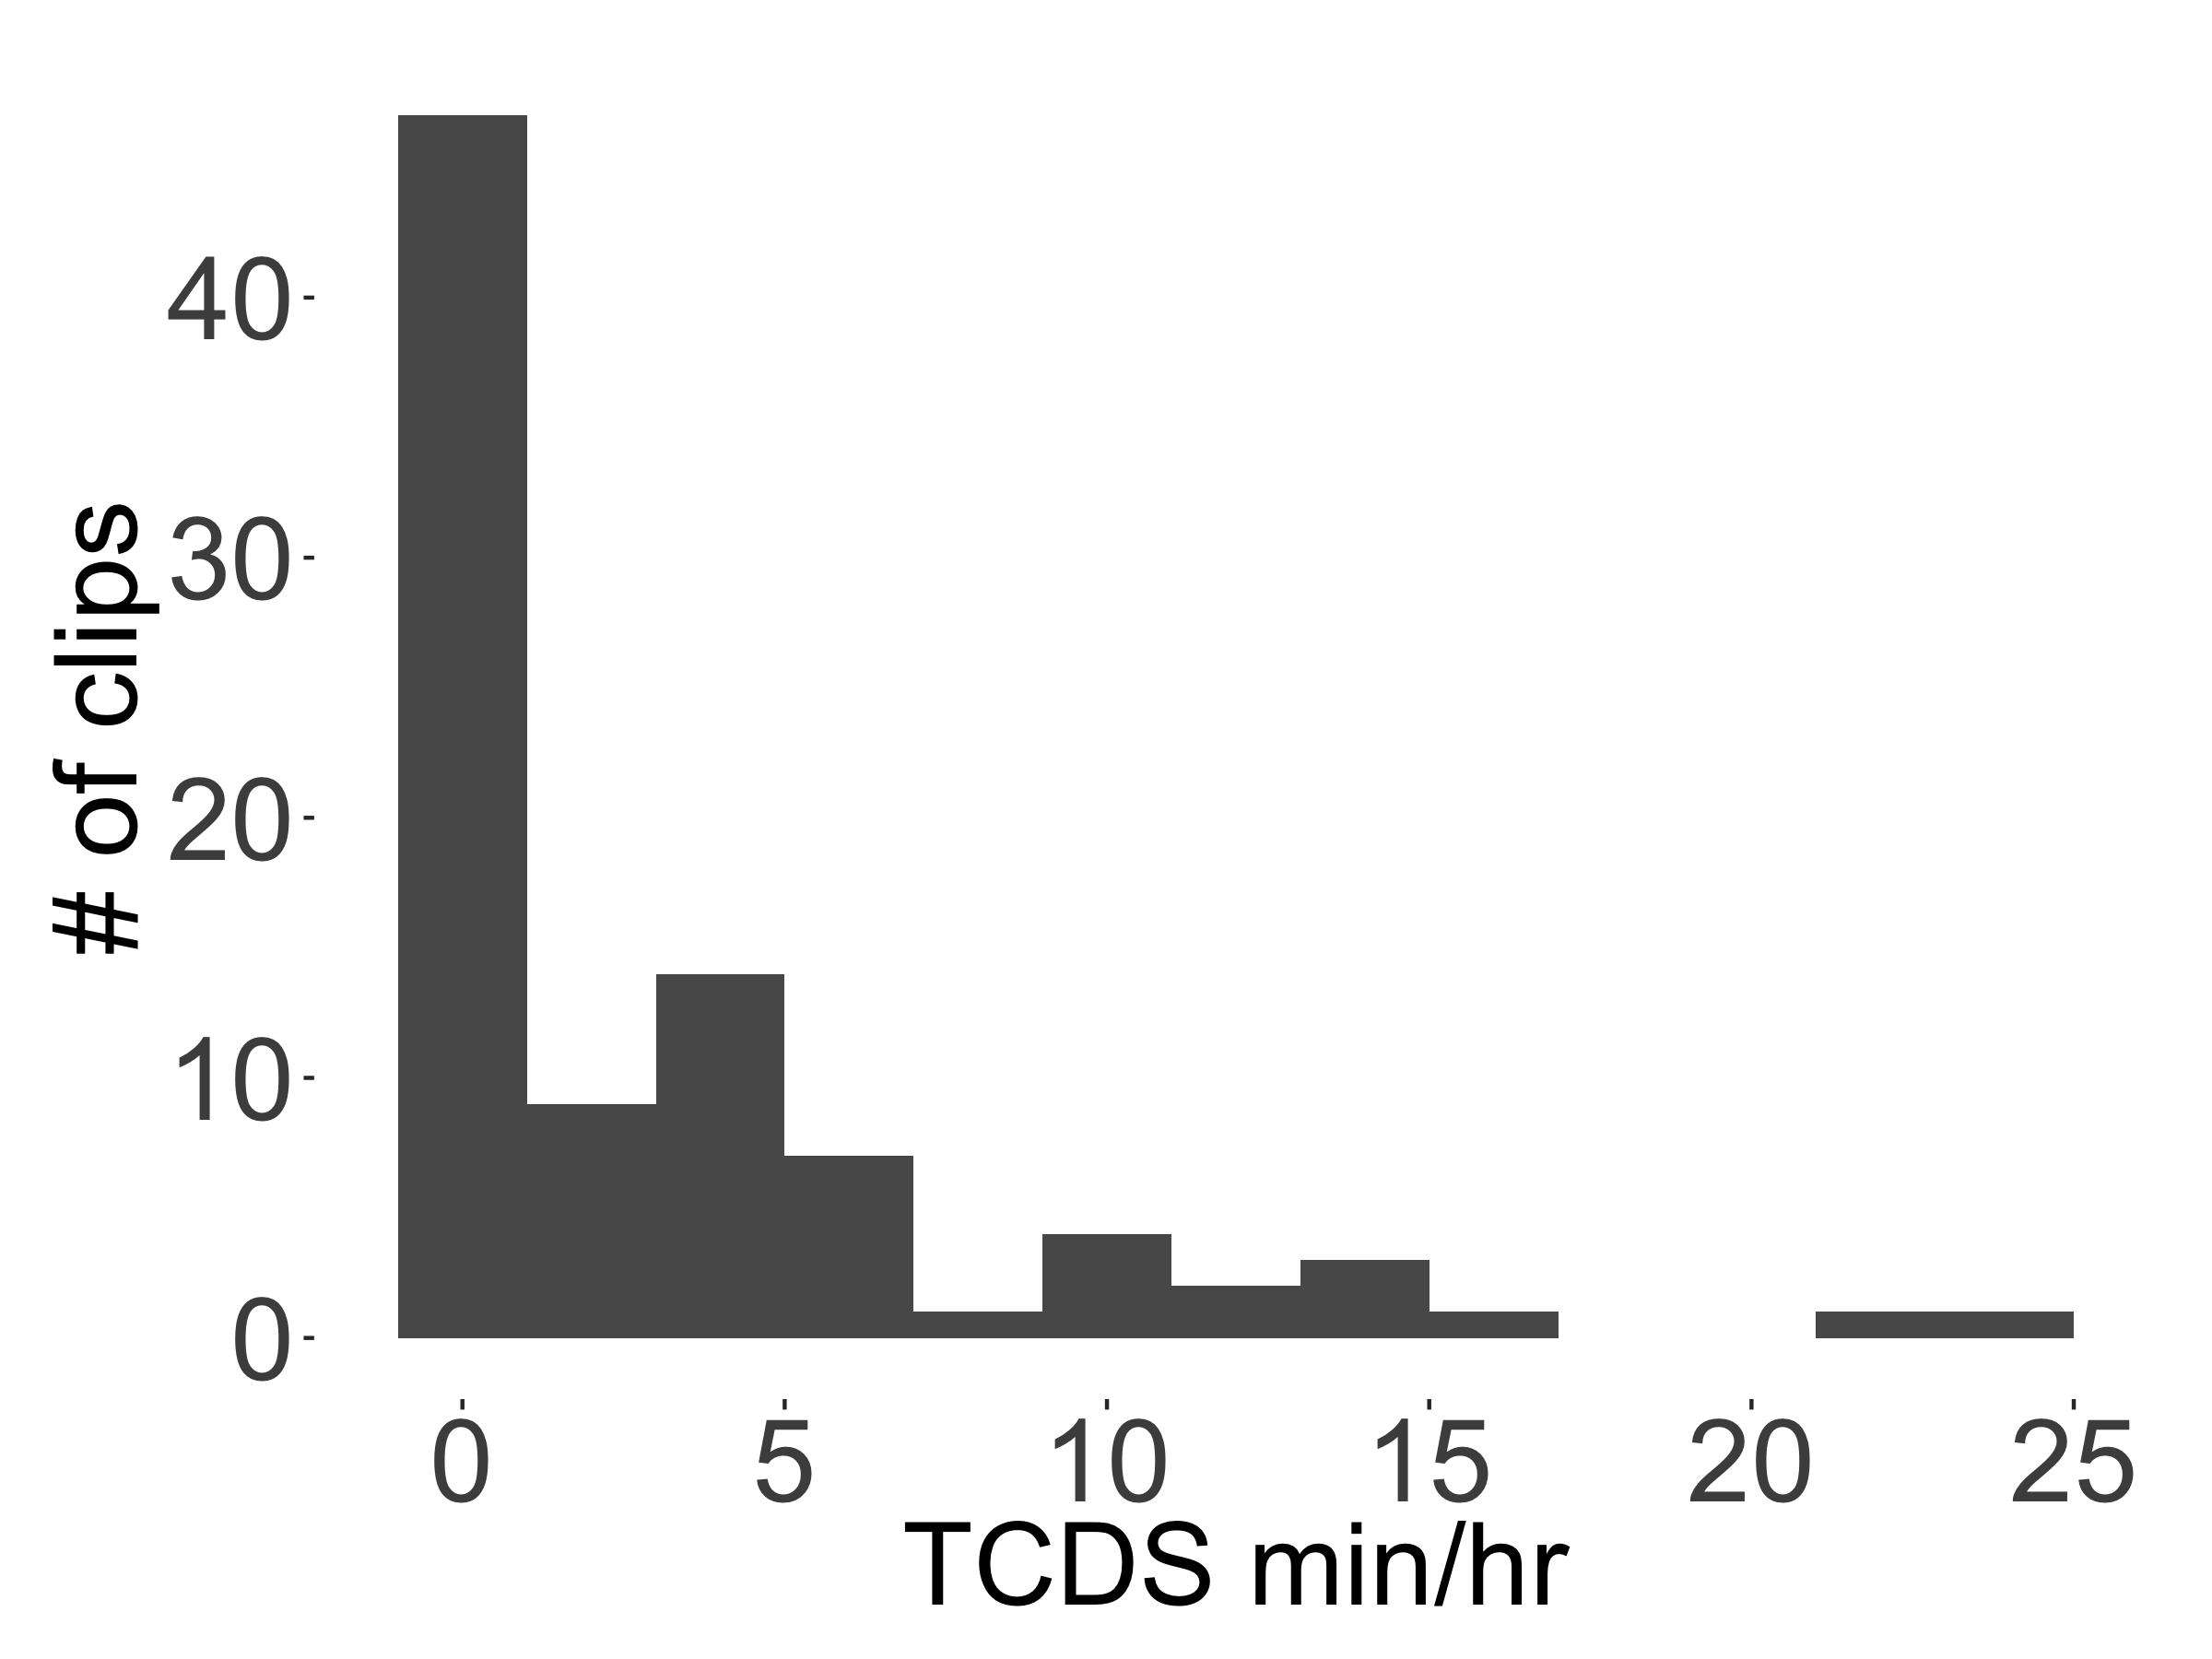
\includegraphics[width=0.4\linewidth]{www/TCDS_random_distribution} 

}

\caption{The distribution of TCDS rates found across the 90 random clips.}\label{fig:fig1}
\end{figure}

\FloatBarrier

\begin{table}[tbp]
\begin{center}
\begin{threeparttable}
\caption{\label{tab:tab1}Full output of the zero-inflated negative binomial mixed-effects regression of TCDS min/hr for the random sample.}
\begin{tabular}{llllll}
\toprule
component & \multicolumn{1}{c}{term} & \multicolumn{1}{c}{estimate} & \multicolumn{1}{c}{std.error} & \multicolumn{1}{c}{statistic} & \multicolumn{1}{c}{p.value}\\
\midrule
cond & (Intercept) & 0.82 & 0.39 & 2.12 & 0.03\\
cond & tchiyr.std & 0.44 & 0.42 & 1.05 & 0.29\\
cond & stthr.trimorning & 0.82 & 0.40 & 2.06 & 0.04\\
cond & stthr.triafternoon & 0.49 & 0.37 & 1.31 & 0.19\\
cond & hsz.std & -0.09 & 0.26 & -0.33 & 0.74\\
cond & nsk.std & -0.13 & 0.16 & -0.79 & 0.43\\
cond & tchiyr.std:stthr.trimorning & -0.24 & 0.39 & -0.60 & 0.55\\
cond & tchiyr.std:stthr.triafternoon & -0.81 & 0.38 & -2.15 & 0.03\\
cond & tchiyr.std:hsz.std & -0.21 & 0.32 & -0.66 & 0.51\\
cond & tchiyr.std:nsk.std & 0.61 & 0.20 & 3.06 & 0.00\\
zi & (Intercept) & -56.90 & 14,003.31 & 0.00 & 1.00\\
zi & nsk.std & -55.17 & 14,243.76 & 0.00 & 1.00\\
random\_effect & aclew\_child\_id & 0.30 & NA & NA & NA\\
\bottomrule
\end{tabular}
\end{threeparttable}
\end{center}
\end{table}

\begin{table}[tbp]
\begin{center}
\begin{threeparttable}
\caption{\label{tab:tab2}Model output of the zero-inflated negative binomial mixed-effects regression of TCDS min/hr for the random sample, with afternoon as the reference level for time of day.}
\begin{tabular}{llllll}
\toprule
component & \multicolumn{1}{c}{term} & \multicolumn{1}{c}{estimate} & \multicolumn{1}{c}{std.error} & \multicolumn{1}{c}{statistic} & \multicolumn{1}{c}{p.value}\\
\midrule
cond & (Intercept) & 1.36 & 0.23 & 5.88 & 0.00\\
cond & tchiyr.std & -0.31 & 0.25 & -1.22 & 0.22\\
cond & stthr.tri.amidday & -0.49 & 0.38 & -1.29 & 0.20\\
cond & stthr.tri.amorning & 0.30 & 0.29 & 1.06 & 0.29\\
cond & hsz.std & -0.09 & 0.22 & -0.40 & 0.69\\
cond & nsk.std & -0.11 & 0.18 & -0.60 & 0.55\\
cond & tchiyr.std:stthr.tri.amidday & 0.73 & 0.36 & 2.04 & 0.04\\
cond & tchiyr.std:stthr.tri.amorning & 0.46 & 0.28 & 1.65 & 0.10\\
cond & tchiyr.std:hsz.std & -0.20 & 0.26 & -0.76 & 0.45\\
cond & tchiyr.std:nsk.std & 0.57 & 0.20 & 2.83 & 0.00\\
zi & (Intercept) & -58.40 & 13,710.05 & 0.00 & 1.00\\
zi & nsk.std & -56.19 & 13,945.46 & 0.00 & 1.00\\
random\_effect & aclew\_child\_id & 0.00 & NA & NA & NA\\
\bottomrule
\end{tabular}
\end{threeparttable}
\end{center}
\end{table}

\FloatBarrier

\begin{figure}[H]

{\centering 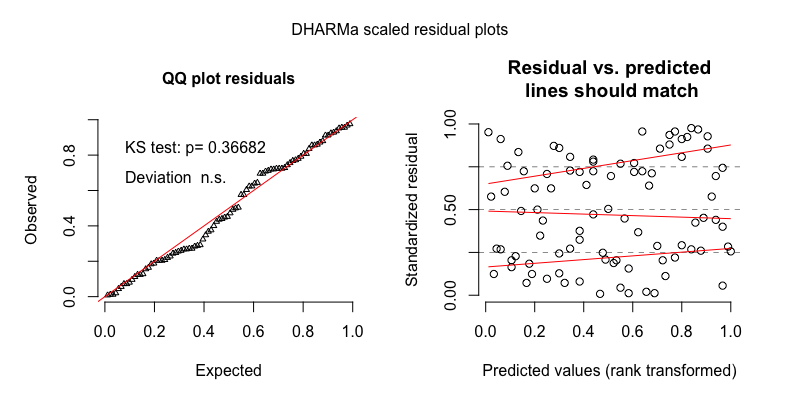
\includegraphics[width=0.9\linewidth]{www/TCDS_random_z-inb_res_plot} 

}

\caption{The model residuals from the zero-inflated negative binomial mixed-effects regression of TCDS min/hr for the random sample.}\label{fig:fig2}
\end{figure}

\FloatBarrier

\begin{table}[tbp]
\begin{center}
\begin{threeparttable}
\caption{\label{tab:tab3}Full output of the gaussian mixed-effects regression of TCDS min/hr for the random sample, with midday as the reference level for time of day.}
\begin{tabular}{llllll}
\toprule
component & \multicolumn{1}{c}{term} & \multicolumn{1}{c}{estimate} & \multicolumn{1}{c}{std.error} & \multicolumn{1}{c}{statistic} & \multicolumn{1}{c}{p.value}\\
\midrule
cond & (Intercept) & 0.78 & 0.22 & 3.44 & 0.00\\
cond & tchiyr.std & 0.49 & 0.26 & 1.90 & 0.06\\
cond & stthr.trimorning & 0.51 & 0.25 & 2.03 & 0.04\\
cond & stthr.triafternoon & 0.29 & 0.22 & 1.32 & 0.18\\
cond & hsz.std & -0.20 & 0.20 & -1.00 & 0.32\\
cond & nsk.std & 0.23 & 0.12 & 1.96 & 0.05\\
cond & tchiyr.std:stthr.trimorning & -0.16 & 0.27 & -0.59 & 0.55\\
cond & tchiyr.std:stthr.triafternoon & -0.68 & 0.24 & -2.85 & 0.00\\
cond & tchiyr.std:hsz.std & -0.08 & 0.24 & -0.36 & 0.72\\
cond & tchiyr.std:nsk.std & 0.25 & 0.15 & 1.68 & 0.09\\
random\_effect & aclew\_child\_id & 0.20 & NA & NA & NA\\
random\_effect & Residual & 0.84 & NA & NA & NA\\
\bottomrule
\end{tabular}
\end{threeparttable}
\end{center}
\end{table}

\begin{table}[tbp]
\begin{center}
\begin{threeparttable}
\caption{\label{tab:tab4}Model output of the gaussian mixed-effects regression of TCDS min/hr for the random sample, with afternoon as the reference level for time of day.}
\begin{tabular}{llllll}
\toprule
component & \multicolumn{1}{c}{term} & \multicolumn{1}{c}{estimate} & \multicolumn{1}{c}{std.error} & \multicolumn{1}{c}{statistic} & \multicolumn{1}{c}{p.value}\\
\midrule
cond & (Intercept) & 1.07 & 0.19 & 5.75 & 0.00\\
cond & tchiyr.std & -0.19 & 0.22 & -0.86 & 0.39\\
cond & stthr.tri.amidday & -0.29 & 0.22 & -1.32 & 0.18\\
cond & stthr.tri.amorning & 0.22 & 0.22 & 0.98 & 0.33\\
cond & hsz.std & -0.20 & 0.20 & -1.00 & 0.32\\
cond & nsk.std & 0.23 & 0.12 & 1.96 & 0.05\\
cond & tchiyr.std:stthr.tri.amidday & 0.68 & 0.24 & 2.85 & 0.00\\
cond & tchiyr.std:stthr.tri.amorning & 0.52 & 0.23 & 2.24 & 0.02\\
cond & tchiyr.std:hsz.std & -0.08 & 0.24 & -0.36 & 0.72\\
cond & tchiyr.std:nsk.std & 0.25 & 0.15 & 1.68 & 0.09\\
random\_effect & aclew\_child\_id & 0.20 & NA & NA & NA\\
random\_effect & Residual & 0.84 & NA & NA & NA\\
\bottomrule
\end{tabular}
\end{threeparttable}
\end{center}
\end{table}

\FloatBarrier

\begin{figure}[H]

{\centering 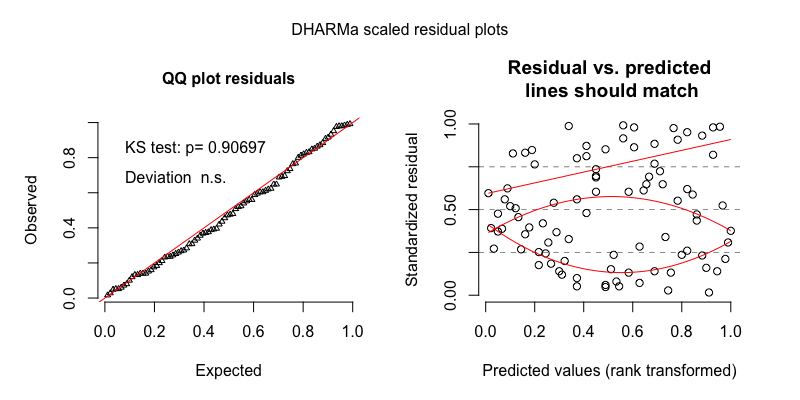
\includegraphics[width=0.9\linewidth]{www/TCDS_random_log_gaus_res_plot} 

}

\caption{The model residuals from the gaussian mixed-effects regression of TCDS min/hr for the random sample.}\label{fig:fig3}
\end{figure}

\FloatBarrier

\subsubsection{Turn-taking clips}\label{models-tcds-turntaking}

TCDS rate in the turn-taking clips demonstrated a fairly normal
distribution. We therefore modeled it using a plain (i.e.,
non-zero-inflated) negative binomial mixed-effects regression.

\FloatBarrier

\begin{figure}[H]

{\centering 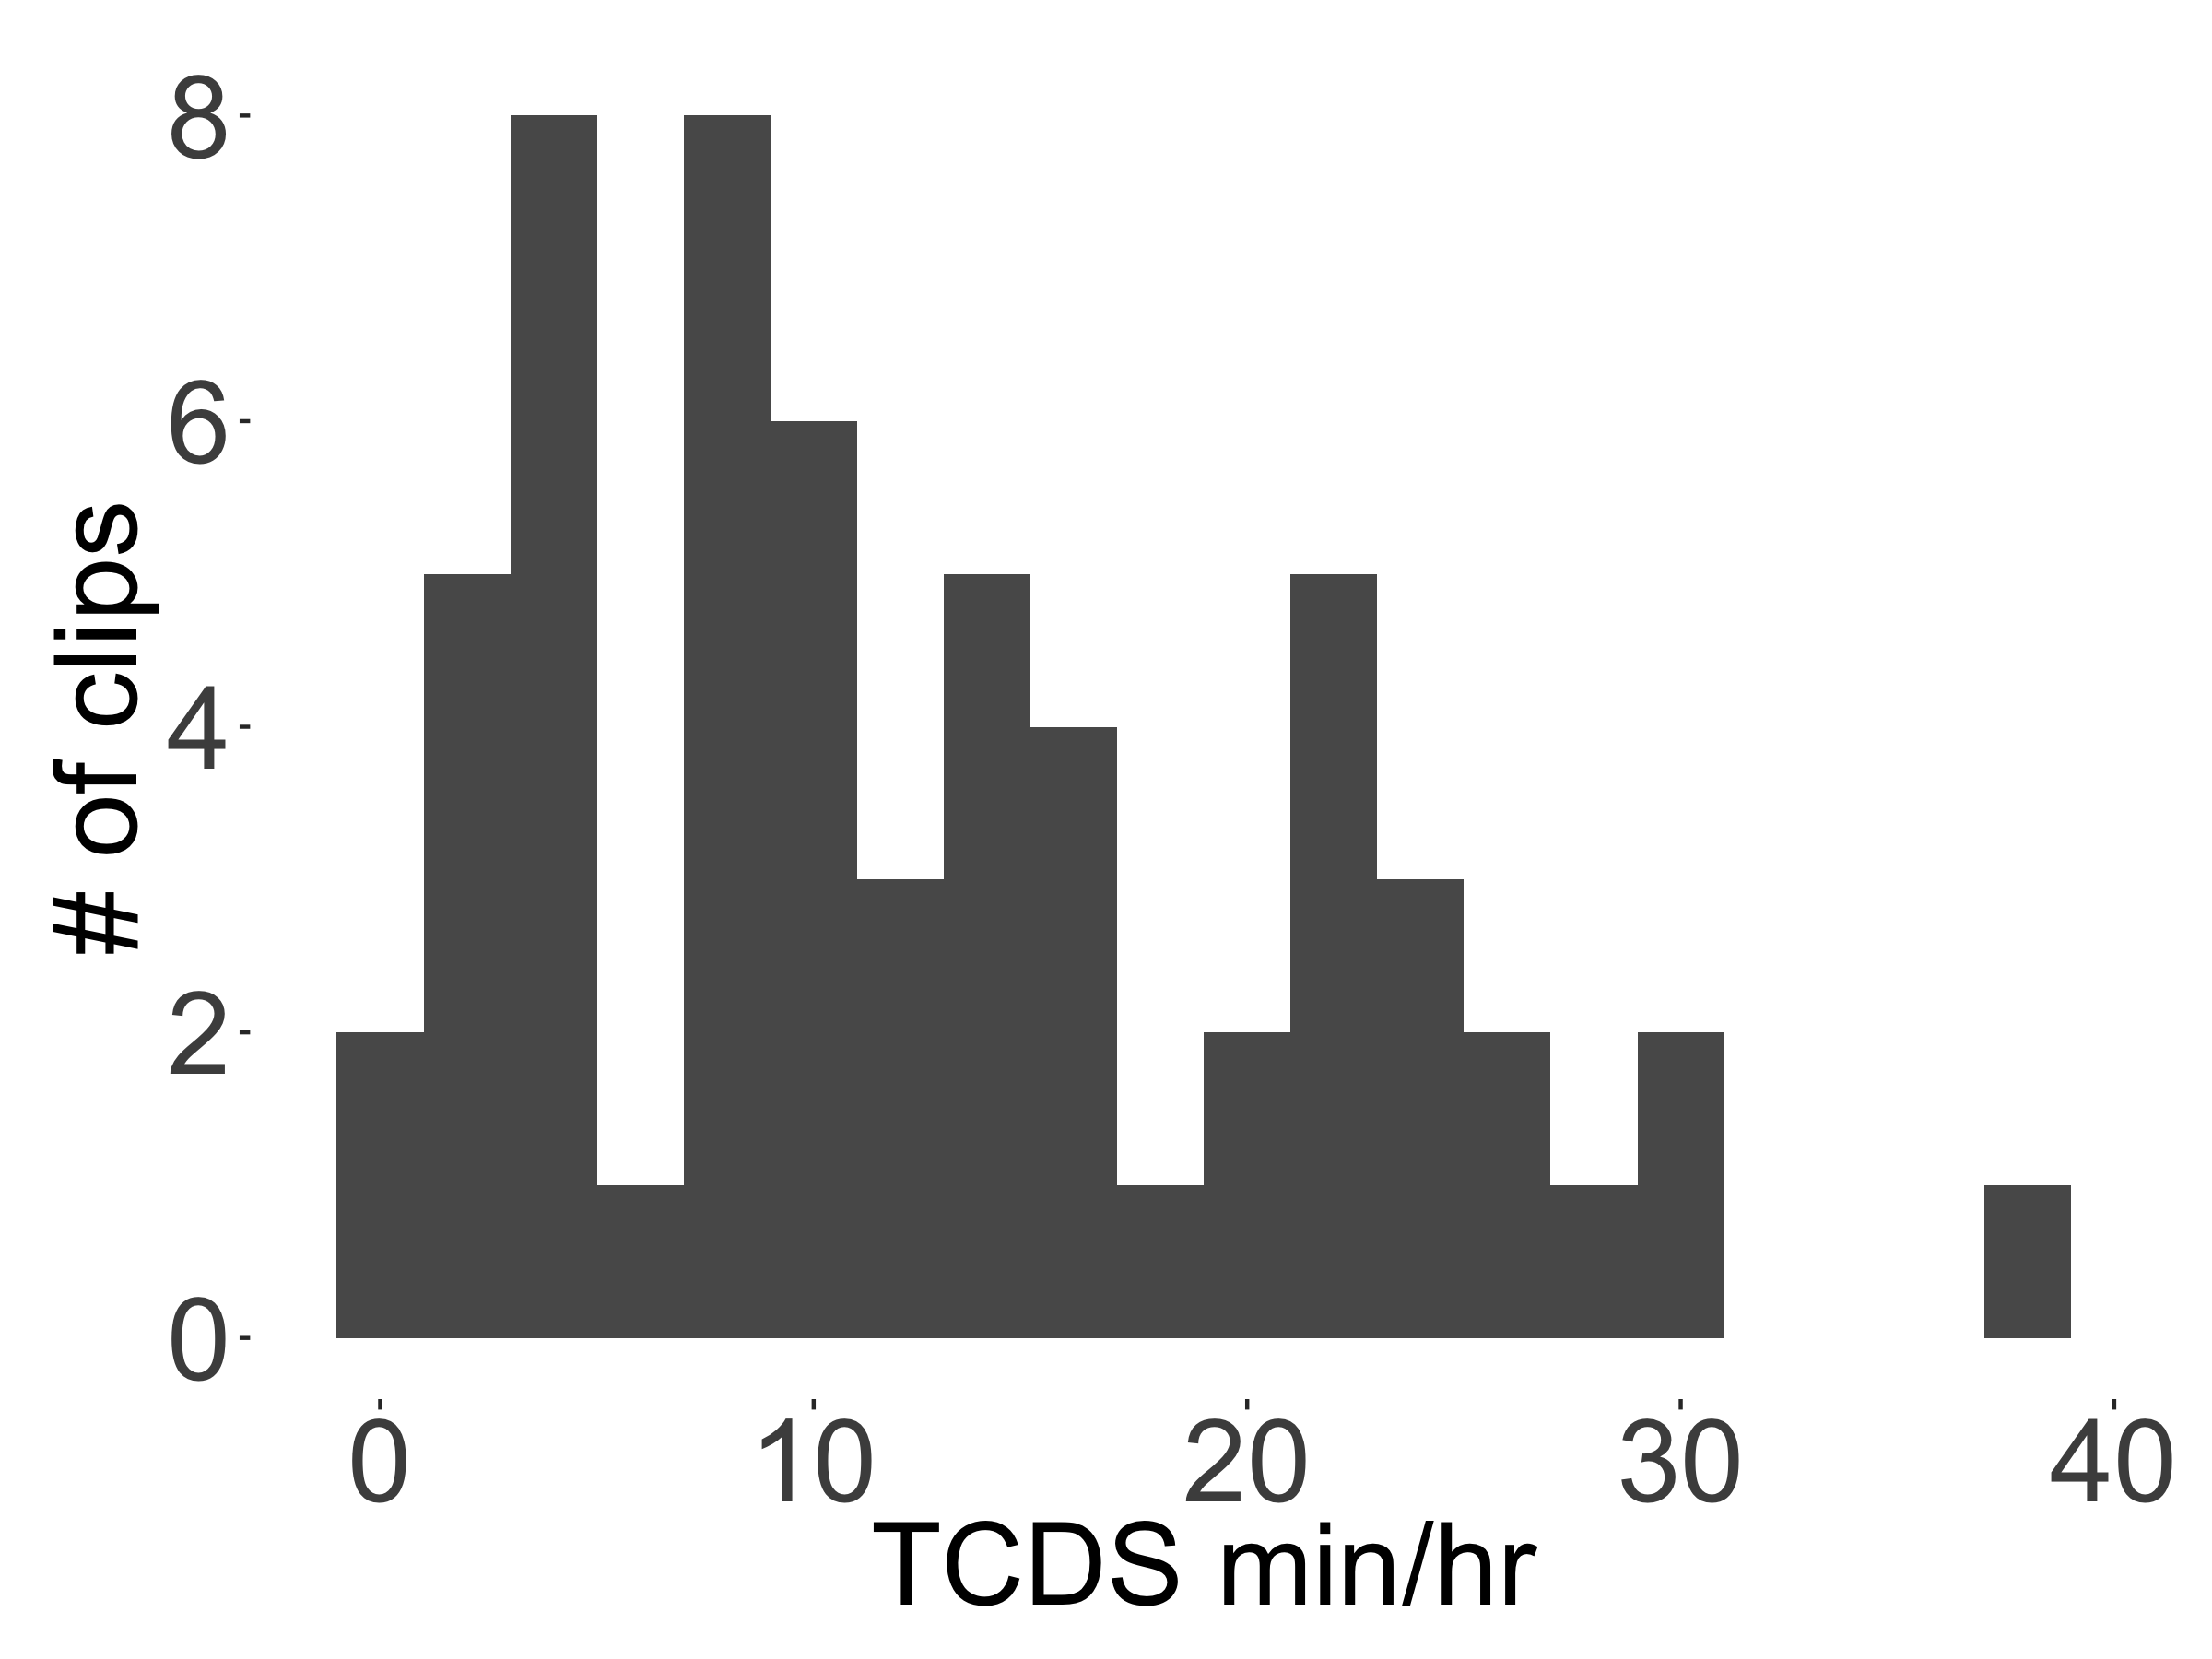
\includegraphics[width=0.4\linewidth]{www/TCDS_turntaking_distribution} 

}

\caption{The distribution of TCDS rates found across the 90 turn-taking clips.}\label{fig:fig4}
\end{figure}

\FloatBarrier

\begin{table}[tbp]
\begin{center}
\begin{threeparttable}
\caption{\label{tab:tab5}Full output of the negative binomial mixed-effects regression of TCDS min/hr for the turn-taking sample.}
\begin{tabular}{llllll}
\toprule
component & \multicolumn{1}{c}{term} & \multicolumn{1}{c}{estimate} & \multicolumn{1}{c}{std.error} & \multicolumn{1}{c}{statistic} & \multicolumn{1}{c}{p.value}\\
\midrule
cond & (Intercept) & 2.22 & 0.23 & 9.85 & 0.00\\
cond & tchiyr.std & -0.16 & 0.21 & -0.77 & 0.44\\
cond & stthr.trimorning & 0.33 & 0.25 & 1.32 & 0.19\\
cond & stthr.triafternoon & 0.06 & 0.23 & 0.28 & 0.78\\
cond & hsz.std & -0.16 & 0.16 & -1.01 & 0.31\\
cond & nsk.std & -0.10 & 0.10 & -0.96 & 0.33\\
cond & tchiyr.std:stthr.trimorning & -0.27 & 0.25 & -1.10 & 0.27\\
cond & tchiyr.std:stthr.triafternoon & -0.03 & 0.21 & -0.16 & 0.88\\
cond & tchiyr.std:hsz.std & -0.49 & 0.20 & -2.42 & 0.02\\
cond & tchiyr.std:nsk.std & 0.14 & 0.12 & 1.15 & 0.25\\
random\_effect & aclew\_child\_id & 0.00 & NA & NA & NA\\
\bottomrule
\end{tabular}
\end{threeparttable}
\end{center}
\end{table}

\begin{table}[tbp]
\begin{center}
\begin{threeparttable}
\caption{\label{tab:tab6}Model output of the negative binomial mixed-effects regression of TCDS min/hr for the turn-taking sample, with afternoon as the reference level for time of day.}
\begin{tabular}{llllll}
\toprule
component & \multicolumn{1}{c}{term} & \multicolumn{1}{c}{estimate} & \multicolumn{1}{c}{std.error} & \multicolumn{1}{c}{statistic} & \multicolumn{1}{c}{p.value}\\
\midrule
cond & (Intercept) & 2.29 & 0.20 & 11.32 & 0.00\\
cond & tchiyr.std & -0.19 & 0.20 & -0.95 & 0.34\\
cond & stthr.tri.amidday & -0.06 & 0.23 & -0.28 & 0.78\\
cond & stthr.tri.amorning & 0.27 & 0.22 & 1.24 & 0.22\\
cond & hsz.std & -0.16 & 0.16 & -1.01 & 0.31\\
cond & nsk.std & -0.10 & 0.10 & -0.96 & 0.33\\
cond & tchiyr.std:stthr.tri.amidday & 0.03 & 0.21 & 0.16 & 0.88\\
cond & tchiyr.std:stthr.tri.amorning & -0.24 & 0.22 & -1.10 & 0.27\\
cond & tchiyr.std:hsz.std & -0.49 & 0.20 & -2.42 & 0.02\\
cond & tchiyr.std:nsk.std & 0.14 & 0.12 & 1.15 & 0.25\\
random\_effect & aclew\_child\_id & 0.00 & NA & NA & NA\\
\bottomrule
\end{tabular}
\end{threeparttable}
\end{center}
\end{table}

\FloatBarrier

\begin{figure}[H]

{\centering 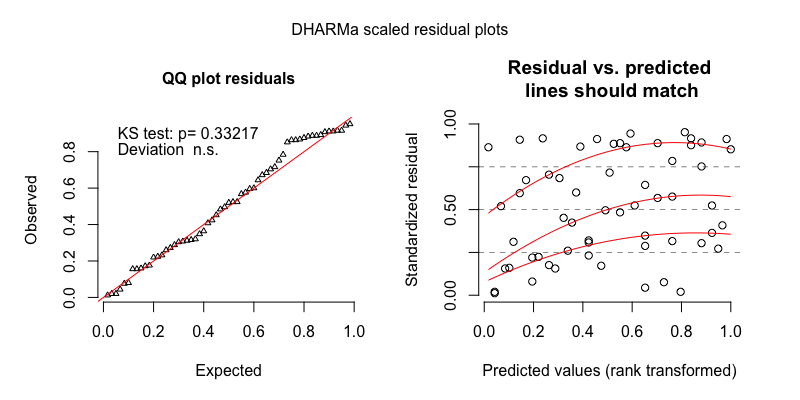
\includegraphics[width=0.9\linewidth]{www/TCDS_turntaking_nb_res_plot} 

}

\caption{The model residuals from the zero-inflated negative binomial mixed-effects regression of TCDS min/hr for the turn-taking sample.}\label{fig:fig5}
\end{figure}

\FloatBarrier

\begin{table}[tbp]
\begin{center}
\begin{threeparttable}
\caption{\label{tab:tab7}Full output of the gaussian mixed-effects regression of TCDS min/hr for the turn-taking sample, with midday as the reference level for time of day.}
\begin{tabular}{llllll}
\toprule
component & \multicolumn{1}{c}{term} & \multicolumn{1}{c}{estimate} & \multicolumn{1}{c}{std.error} & \multicolumn{1}{c}{statistic} & \multicolumn{1}{c}{p.value}\\
\midrule
cond & (Intercept) & 2.08 & 0.24 & 8.55 & 0.00\\
cond & tchiyr.std & -0.13 & 0.23 & -0.55 & 0.58\\
cond & stthr.trimorning & 0.38 & 0.30 & 1.28 & 0.20\\
cond & stthr.triafternoon & 0.11 & 0.27 & 0.40 & 0.69\\
cond & hsz.std & -0.15 & 0.17 & -0.85 & 0.39\\
cond & nsk.std & -0.08 & 0.12 & -0.67 & 0.50\\
cond & tchiyr.std:stthr.trimorning & -0.34 & 0.30 & -1.16 & 0.24\\
cond & tchiyr.std:stthr.triafternoon & 0.00 & 0.26 & -0.02 & 0.99\\
cond & tchiyr.std:hsz.std & -0.49 & 0.22 & -2.24 & 0.02\\
cond & tchiyr.std:nsk.std & 0.17 & 0.15 & 1.13 & 0.26\\
random\_effect & aclew\_child\_id & 0.00 & NA & NA & NA\\
random\_effect & Residual & 0.71 & NA & NA & NA\\
\bottomrule
\end{tabular}
\end{threeparttable}
\end{center}
\end{table}

\begin{table}[tbp]
\begin{center}
\begin{threeparttable}
\caption{\label{tab:tab8}Model output of the gaussian mixed-effects regression of TCDS min/hr for the turn-taking sample, with afternoon as the reference level for time of day.}
\begin{tabular}{llllll}
\toprule
component & \multicolumn{1}{c}{term} & \multicolumn{1}{c}{estimate} & \multicolumn{1}{c}{std.error} & \multicolumn{1}{c}{statistic} & \multicolumn{1}{c}{p.value}\\
\midrule
cond & (Intercept) & 2.19 & 0.21 & 10.47 & 0.00\\
cond & tchiyr.std & -0.13 & 0.23 & -0.58 & 0.56\\
cond & stthr.tri.amidday & -0.11 & 0.27 & -0.40 & 0.69\\
cond & stthr.tri.amorning & 0.28 & 0.26 & 1.04 & 0.30\\
cond & hsz.std & -0.15 & 0.17 & -0.85 & 0.39\\
cond & nsk.std & -0.08 & 0.12 & -0.67 & 0.50\\
cond & tchiyr.std:stthr.tri.amidday & 0.00 & 0.26 & 0.02 & 0.99\\
cond & tchiyr.std:stthr.tri.amorning & -0.34 & 0.28 & -1.23 & 0.22\\
cond & tchiyr.std:hsz.std & -0.49 & 0.22 & -2.24 & 0.02\\
cond & tchiyr.std:nsk.std & 0.17 & 0.15 & 1.13 & 0.26\\
random\_effect & aclew\_child\_id & 0.00 & NA & NA & NA\\
random\_effect & Residual & 0.71 & NA & NA & NA\\
\bottomrule
\end{tabular}
\end{threeparttable}
\end{center}
\end{table}

\FloatBarrier

\begin{figure}[H]

{\centering 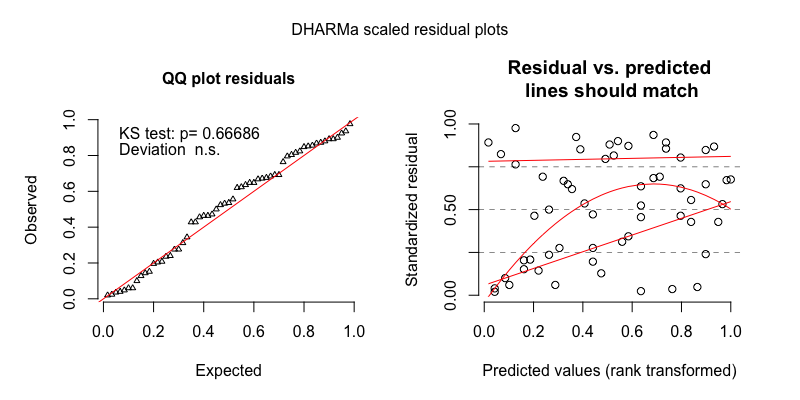
\includegraphics[width=0.9\linewidth]{www/TCDS_turntaking_log_gaus_res_plot} 

}

\caption{The model residuals from the gaussian mixed-effects regression of TCDS min/hr for the turn-taking sample.}\label{fig:fig6}
\end{figure}

\FloatBarrier

\subsection{Other-directed speech (ODS)}\label{models-ods}

\subsubsection{Random clips}\label{models-ods-random}

ODS rate in the random clips demonstrated a skewed distribution with
extra cases of zero. We therefore modeled it using a zero-inflated
negative binomial mixed-effects regression.

\FloatBarrier

\begin{figure}[H]

{\centering 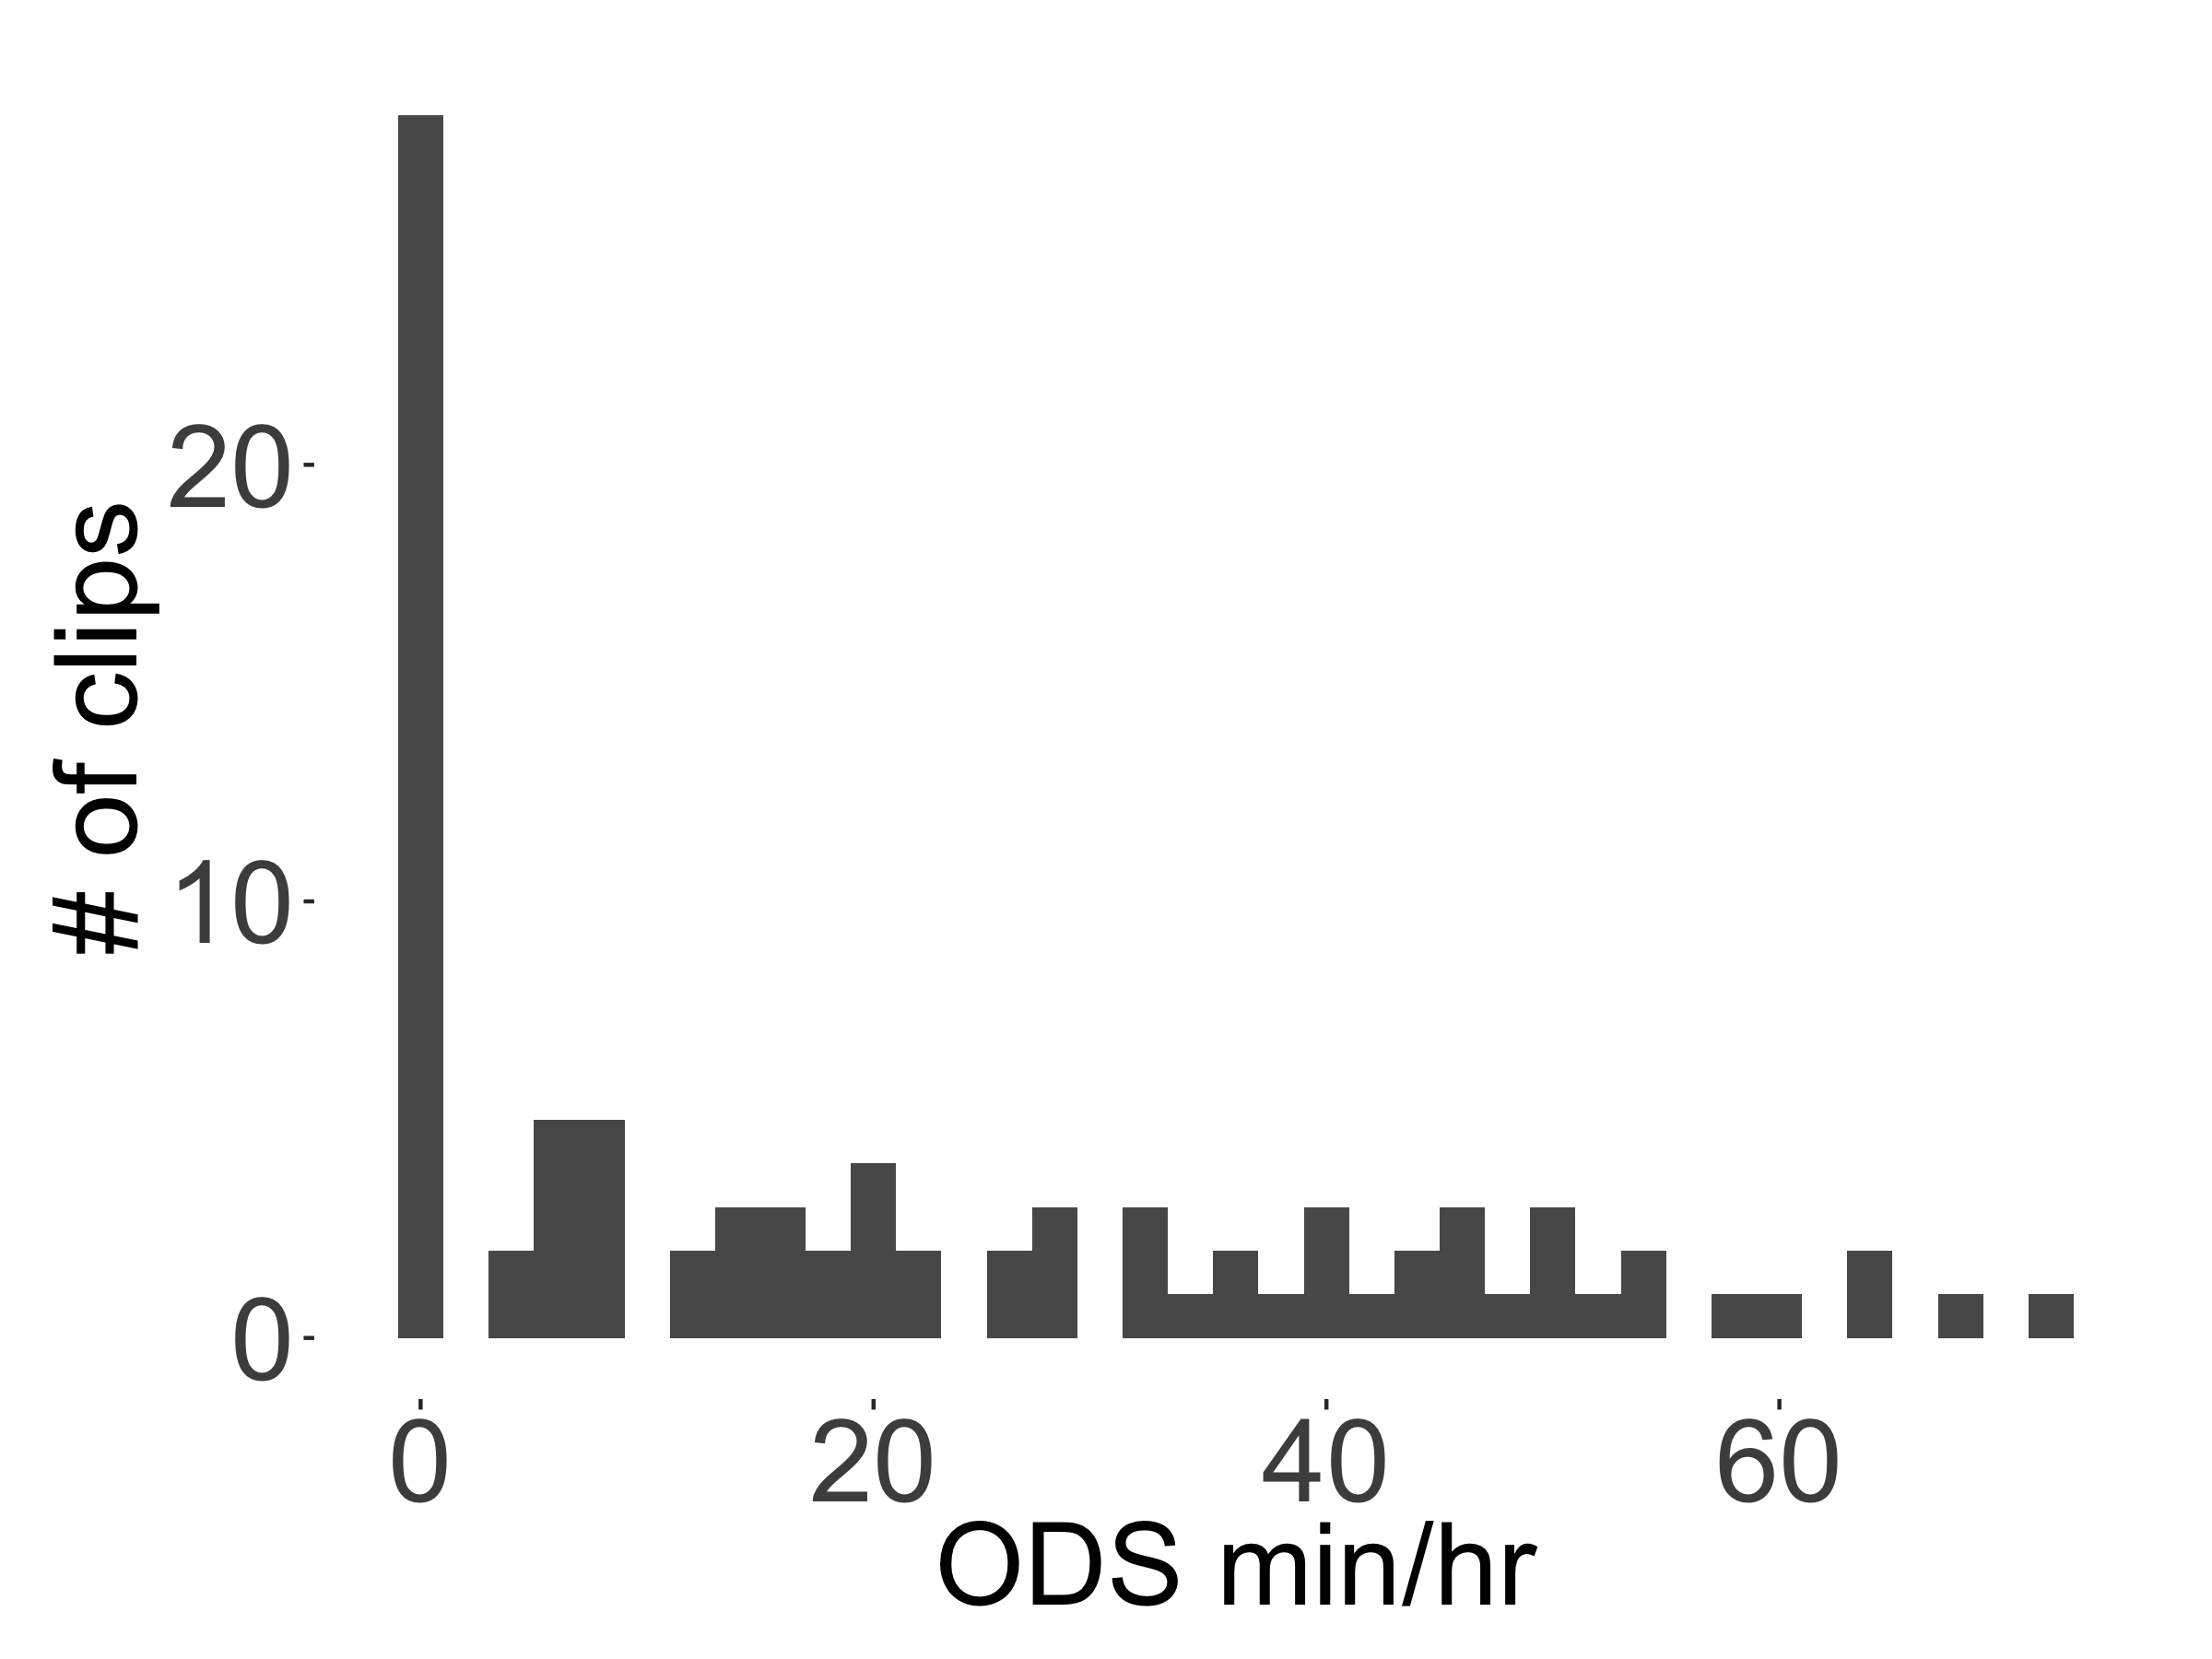
\includegraphics[width=0.4\linewidth]{www/ODS_random_distribution} 

}

\caption{The distribution of ODS rates found across the 90 random clips.}\label{fig:fig7}
\end{figure}

\FloatBarrier

\begin{table}[tbp]
\begin{center}
\begin{threeparttable}
\caption{\label{tab:tab9}Full output of the zero-inflated negative binomial mixed-effects regression of ODS min/hr for the random sample.}
\begin{tabular}{llllll}
\toprule
component & \multicolumn{1}{c}{term} & \multicolumn{1}{c}{estimate} & \multicolumn{1}{c}{std.error} & \multicolumn{1}{c}{statistic} & \multicolumn{1}{c}{p.value}\\
\midrule
cond & (Intercept) & 2.87 & 0.16 & 17.95 & 0.00\\
cond & tchiyr.std & -0.13 & 0.18 & -0.70 & 0.49\\
cond & stthr.trimorning & 0.36 & 0.17 & 2.09 & 0.04\\
cond & stthr.triafternoon & 0.29 & 0.16 & 1.89 & 0.06\\
cond & hsz.std & 0.04 & 0.10 & 0.44 & 0.66\\
cond & nsk.std & 0.65 & 0.09 & 7.33 & 0.00\\
cond & tchiyr.std:stthr.trimorning & 0.10 & 0.21 & 0.48 & 0.63\\
cond & tchiyr.std:stthr.triafternoon & 0.38 & 0.17 & 2.21 & 0.03\\
cond & tchiyr.std:hsz.std & 0.32 & 0.13 & 2.41 & 0.02\\
cond & tchiyr.std:nsk.std & -0.02 & 0.13 & -0.15 & 0.88\\
zi & (Intercept) & -50.25 & 10,421.88 & 0.00 & 1.00\\
zi & nsk.std & -53.76 & 10,600.83 & 0.00 & 1.00\\
random\_effect & aclew\_child\_id & 0.00 & NA & NA & NA\\
\bottomrule
\end{tabular}
\end{threeparttable}
\end{center}
\end{table}

\begin{table}[tbp]
\begin{center}
\begin{threeparttable}
\caption{\label{tab:tab10}Model output of the zero-inflated negative binomial mixed-effects regression of ODS min/hr for the random sample, with afternoon as the reference level for time of day.}
\begin{tabular}{llllll}
\toprule
component & \multicolumn{1}{c}{term} & \multicolumn{1}{c}{estimate} & \multicolumn{1}{c}{std.error} & \multicolumn{1}{c}{statistic} & \multicolumn{1}{c}{p.value}\\
\midrule
cond & (Intercept) & 3.16 & 0.11 & 28.09 & 0.00\\
cond & tchiyr.std & 0.25 & 0.14 & 1.84 & 0.07\\
cond & stthr.tri.amidday & -0.29 & 0.16 & -1.89 & 0.06\\
cond & stthr.tri.amorning & 0.07 & 0.14 & 0.48 & 0.63\\
cond & hsz.std & 0.04 & 0.10 & 0.44 & 0.66\\
cond & nsk.std & 0.65 & 0.09 & 7.33 & 0.00\\
cond & tchiyr.std:stthr.tri.amidday & -0.38 & 0.17 & -2.21 & 0.03\\
cond & tchiyr.std:stthr.tri.amorning & -0.28 & 0.17 & -1.62 & 0.10\\
cond & tchiyr.std:hsz.std & 0.32 & 0.13 & 2.41 & 0.02\\
cond & tchiyr.std:nsk.std & -0.02 & 0.13 & -0.15 & 0.88\\
zi & (Intercept) & -50.71 & 11,450.44 & 0.00 & 1.00\\
zi & nsk.std & -54.22 & 11,647.05 & 0.00 & 1.00\\
random\_effect & aclew\_child\_id & 0.00 & NA & NA & NA\\
\bottomrule
\end{tabular}
\end{threeparttable}
\end{center}
\end{table}

\FloatBarrier

\begin{figure}[H]

{\centering 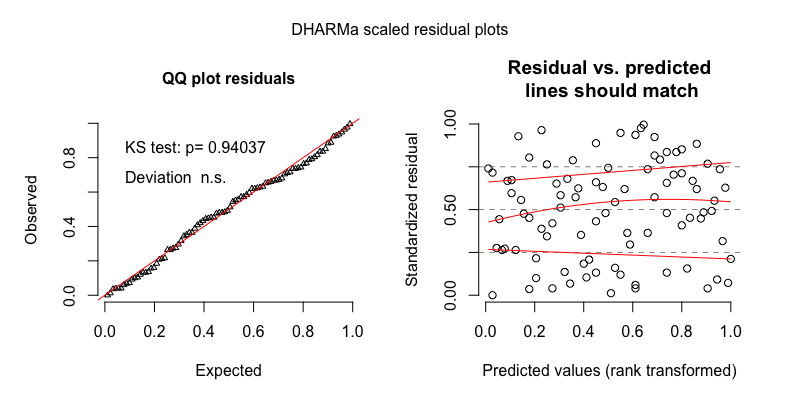
\includegraphics[width=0.9\linewidth]{www/ODS_random_z-inb_res_plot} 

}

\caption{The model residuals from the zero-inflated negative binomial mixed-effects regression of ODS min/hr for the random sample.}\label{fig:fig8}
\end{figure}

\FloatBarrier

\begin{table}[tbp]
\begin{center}
\begin{threeparttable}
\caption{\label{tab:tab11}Full output of the gaussian mixed-effects regression of ODS min/hr for the random sample, with midday as the reference level for time of day.}
\begin{tabular}{llllll}
\toprule
component & \multicolumn{1}{c}{term} & \multicolumn{1}{c}{estimate} & \multicolumn{1}{c}{std.error} & \multicolumn{1}{c}{statistic} & \multicolumn{1}{c}{p.value}\\
\midrule
cond & (Intercept) & 2.21 & 0.17 & 12.75 & 0.00\\
cond & tchiyr.std & -0.08 & 0.20 & -0.41 & 0.68\\
cond & stthr.trimorning & 0.21 & 0.21 & 1.02 & 0.31\\
cond & stthr.triafternoon & 0.34 & 0.19 & 1.80 & 0.07\\
cond & hsz.std & -0.22 & 0.14 & -1.62 & 0.10\\
cond & nsk.std & 1.53 & 0.09 & 16.25 & 0.00\\
cond & tchiyr.std:stthr.trimorning & -0.01 & 0.23 & -0.03 & 0.98\\
cond & tchiyr.std:stthr.triafternoon & 0.42 & 0.20 & 2.10 & 0.04\\
cond & tchiyr.std:hsz.std & 0.32 & 0.17 & 1.90 & 0.06\\
cond & tchiyr.std:nsk.std & 0.08 & 0.12 & 0.68 & 0.50\\
random\_effect & aclew\_child\_id & 0.00 & NA & NA & NA\\
random\_effect & Residual & 0.72 & NA & NA & NA\\
\bottomrule
\end{tabular}
\end{threeparttable}
\end{center}
\end{table}

\begin{table}[tbp]
\begin{center}
\begin{threeparttable}
\caption{\label{tab:tab12}Model output of the gaussian mixed-effects regression of ODS min/hr for the random sample, with afternoon as the reference level for time of day.}
\begin{tabular}{llllll}
\toprule
component & \multicolumn{1}{c}{term} & \multicolumn{1}{c}{estimate} & \multicolumn{1}{c}{std.error} & \multicolumn{1}{c}{statistic} & \multicolumn{1}{c}{p.value}\\
\midrule
cond & (Intercept) & 2.55 & 0.14 & 18.71 & 0.00\\
cond & tchiyr.std & 0.34 & 0.16 & 2.12 & 0.03\\
cond & stthr.tri.amidday & -0.34 & 0.19 & -1.80 & 0.07\\
cond & stthr.tri.amorning & -0.12 & 0.18 & -0.66 & 0.51\\
cond & hsz.std & -0.22 & 0.14 & -1.62 & 0.10\\
cond & nsk.std & 1.53 & 0.09 & 16.25 & 0.00\\
cond & tchiyr.std:stthr.tri.amidday & -0.42 & 0.20 & -2.10 & 0.04\\
cond & tchiyr.std:stthr.tri.amorning & -0.43 & 0.20 & -2.19 & 0.03\\
cond & tchiyr.std:hsz.std & 0.32 & 0.17 & 1.90 & 0.06\\
cond & tchiyr.std:nsk.std & 0.08 & 0.12 & 0.68 & 0.50\\
random\_effect & aclew\_child\_id & 0.00 & NA & NA & NA\\
random\_effect & Residual & 0.72 & NA & NA & NA\\
\bottomrule
\end{tabular}
\end{threeparttable}
\end{center}
\end{table}

\FloatBarrier

\begin{figure}[H]

{\centering 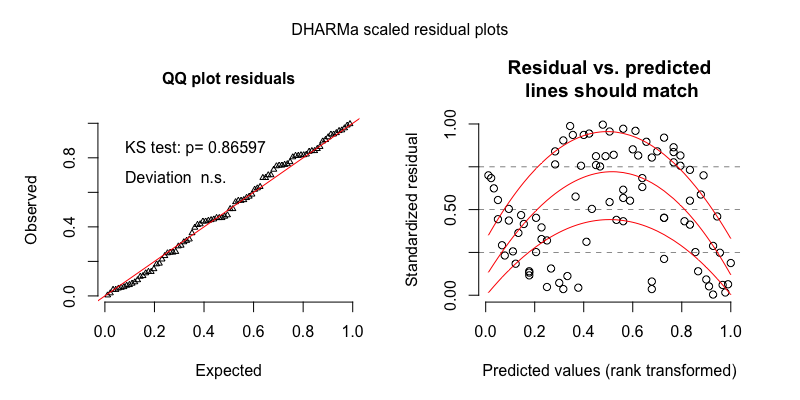
\includegraphics[width=0.9\linewidth]{www/ODS_random_log_gaus_res_plot} 

}

\caption{The model residuals from the gaussian mixed-effects regression of ODS min/hr for the random sample.}\label{fig:fig9}
\end{figure}

\FloatBarrier

\subsubsection{Turn-taking clips}\label{models-ods-turntaking}

ODS rate in the random clips demonstrated a skewed distribution with
extra cases of zero. We therefore modeled it using a zero-inflated
negative binomial mixed-effects regression.

\FloatBarrier

\begin{figure}[H]

{\centering 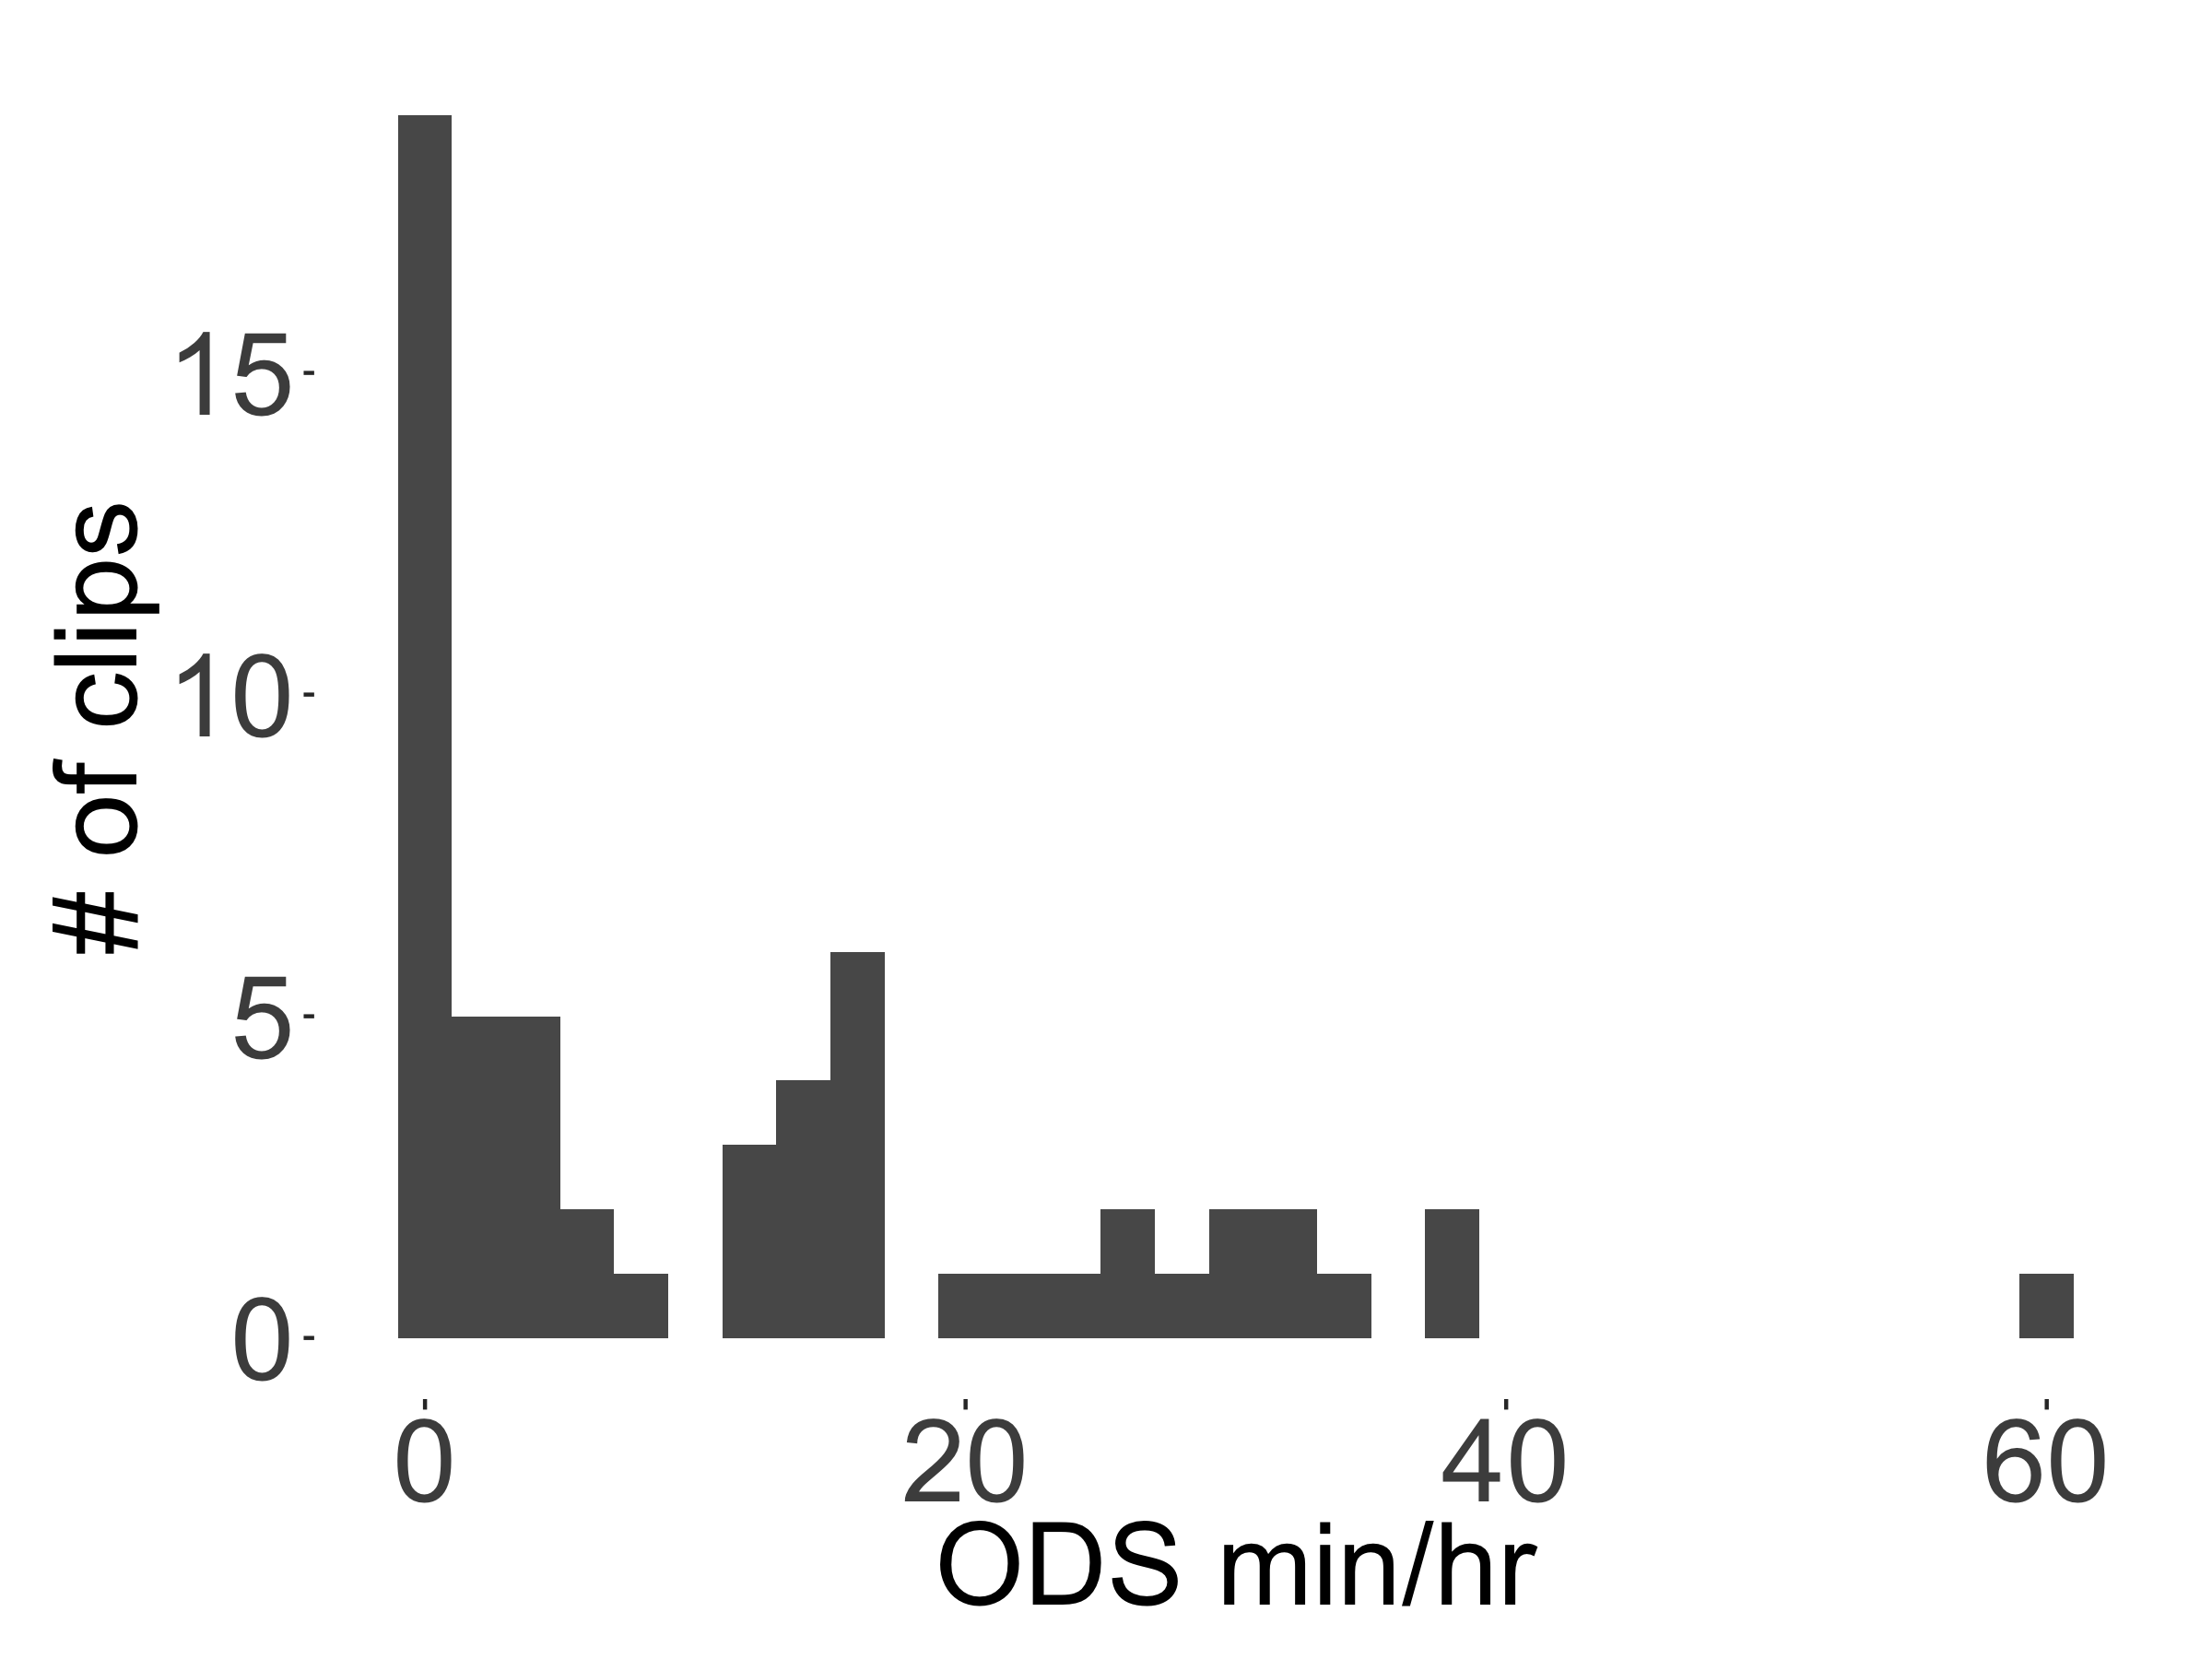
\includegraphics[width=0.4\linewidth]{www/ODS_turntaking_distribution} 

}

\caption{The distribution of ODS rates found across the 90 turn-taking clips.}\label{fig:fig10}
\end{figure}

\FloatBarrier

\begin{table}[tbp]
\begin{center}
\begin{threeparttable}
\caption{\label{tab:tab13}Full output of the negative binomial mixed-effects regression of ODS min/hr for the turn-taking sample.}
\begin{tabular}{llllll}
\toprule
component & \multicolumn{1}{c}{term} & \multicolumn{1}{c}{estimate} & \multicolumn{1}{c}{std.error} & \multicolumn{1}{c}{statistic} & \multicolumn{1}{c}{p.value}\\
\midrule
cond & (Intercept) & 2.47 & 0.22 & 11.29 & 0.00\\
cond & tchiyr.std & -0.45 & 0.20 & -2.19 & 0.03\\
cond & stthr.trimorning & 0.02 & 0.26 & 0.09 & 0.93\\
cond & stthr.triafternoon & -0.70 & 0.29 & -2.39 & 0.02\\
cond & hsz.std & -0.44 & 0.17 & -2.60 & 0.01\\
cond & nsk.std & 0.71 & 0.11 & 6.63 & 0.00\\
cond & tchiyr.std:stthr.trimorning & -0.56 & 0.28 & -1.99 & 0.05\\
cond & tchiyr.std:stthr.triafternoon & -0.14 & 0.30 & -0.47 & 0.64\\
cond & tchiyr.std:hsz.std & -0.38 & 0.22 & -1.74 & 0.08\\
cond & tchiyr.std:nsk.std & 0.10 & 0.14 & 0.73 & 0.47\\
zi & (Intercept) & -32.21 & 12,233.79 & 0.00 & 1.00\\
zi & nsk.std & -31.55 & 12,037.74 & 0.00 & 1.00\\
random\_effect & aclew\_child\_id & 0.00 & NA & NA & NA\\
\bottomrule
\end{tabular}
\end{threeparttable}
\end{center}
\end{table}

\begin{table}[tbp]
\begin{center}
\begin{threeparttable}
\caption{\label{tab:tab14}Model output of the negative binomial mixed-effects regression of ODS min/hr for the turn-taking sample, with afternoon as the reference level for time of day.}
\begin{tabular}{llllll}
\toprule
component & \multicolumn{1}{c}{term} & \multicolumn{1}{c}{estimate} & \multicolumn{1}{c}{std.error} & \multicolumn{1}{c}{statistic} & \multicolumn{1}{c}{p.value}\\
\midrule
cond & (Intercept) & 1.77 & 0.27 & 6.64 & 0.00\\
cond & tchiyr.std & -0.59 & 0.28 & -2.10 & 0.04\\
cond & stthr.tri.amidday & 0.70 & 0.29 & 2.39 & 0.02\\
cond & stthr.tri.amorning & 0.72 & 0.25 & 2.91 & 0.00\\
cond & hsz.std & -0.44 & 0.17 & -2.60 & 0.01\\
cond & nsk.std & 0.71 & 0.11 & 6.63 & 0.00\\
cond & tchiyr.std:stthr.tri.amidday & 0.14 & 0.30 & 0.47 & 0.64\\
cond & tchiyr.std:stthr.tri.amorning & -0.42 & 0.27 & -1.54 & 0.12\\
cond & tchiyr.std:hsz.std & -0.38 & 0.22 & -1.74 & 0.08\\
cond & tchiyr.std:nsk.std & 0.10 & 0.14 & 0.73 & 0.47\\
zi & (Intercept) & -32.46 & 13,260.31 & 0.00 & 1.00\\
zi & nsk.std & -31.79 & 13,047.81 & 0.00 & 1.00\\
random\_effect & aclew\_child\_id & 0.00 & NA & NA & NA\\
\bottomrule
\end{tabular}
\end{threeparttable}
\end{center}
\end{table}

\FloatBarrier

\begin{figure}[H]

{\centering 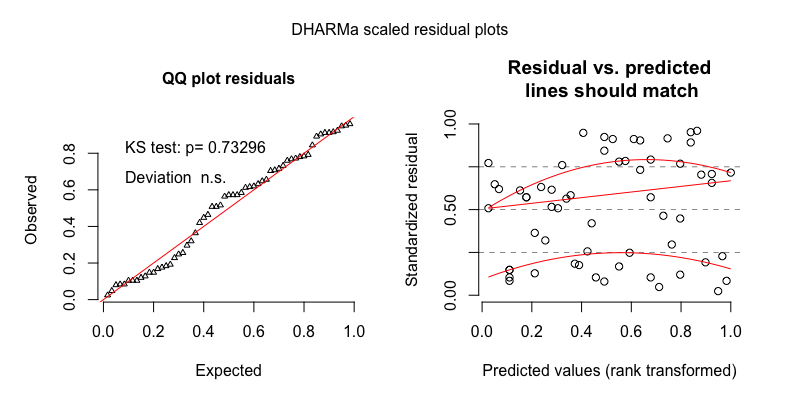
\includegraphics[width=0.9\linewidth]{www/ODS_turntaking_z-inb_res_plot} 

}

\caption{The model residuals from the zero-inflated negative binomial mixed-effects regression of ODS min/hr for the turn-taking sample.}\label{fig:fig11}
\end{figure}

\FloatBarrier

\begin{table}[tbp]
\begin{center}
\begin{threeparttable}
\caption{\label{tab:tab15}Full output of the gaussian mixed-effects regression of ODS min/hr for the turn-taking sample, with midday as the reference level for time of day.}
\begin{tabular}{llllll}
\toprule
component & \multicolumn{1}{c}{term} & \multicolumn{1}{c}{estimate} & \multicolumn{1}{c}{std.error} & \multicolumn{1}{c}{statistic} & \multicolumn{1}{c}{p.value}\\
\midrule
cond & (Intercept) & 2.24 & 0.24 & 9.52 & 0.00\\
cond & tchiyr.std & -0.26 & 0.23 & -1.13 & 0.26\\
cond & stthr.trimorning & -0.19 & 0.29 & -0.65 & 0.51\\
cond & stthr.triafternoon & -0.75 & 0.26 & -2.89 & 0.00\\
cond & hsz.std & -0.39 & 0.17 & -2.32 & 0.02\\
cond & nsk.std & 1.12 & 0.11 & 10.06 & 0.00\\
cond & tchiyr.std:stthr.trimorning & -0.29 & 0.29 & -1.01 & 0.31\\
cond & tchiyr.std:stthr.triafternoon & 0.04 & 0.25 & 0.17 & 0.86\\
cond & tchiyr.std:hsz.std & -0.21 & 0.21 & -1.00 & 0.32\\
cond & tchiyr.std:nsk.std & -0.03 & 0.14 & -0.22 & 0.82\\
random\_effect & aclew\_child\_id & 0.00 & NA & NA & NA\\
random\_effect & Residual & 0.69 & NA & NA & NA\\
\bottomrule
\end{tabular}
\end{threeparttable}
\end{center}
\end{table}

\begin{table}[tbp]
\begin{center}
\begin{threeparttable}
\caption{\label{tab:tab16}Model output of the gaussian mixed-effects regression of ODS min/hr for the turn-taking sample, with afternoon as the reference level for time of day.}
\begin{tabular}{llllll}
\toprule
component & \multicolumn{1}{c}{term} & \multicolumn{1}{c}{estimate} & \multicolumn{1}{c}{std.error} & \multicolumn{1}{c}{statistic} & \multicolumn{1}{c}{p.value}\\
\midrule
cond & (Intercept) & 1.49 & 0.20 & 7.38 & 0.00\\
cond & tchiyr.std & -0.21 & 0.22 & -0.96 & 0.34\\
cond & stthr.tri.amidday & 0.75 & 0.26 & 2.89 & 0.00\\
cond & stthr.tri.amorning & 0.56 & 0.26 & 2.18 & 0.03\\
cond & hsz.std & -0.39 & 0.17 & -2.32 & 0.02\\
cond & nsk.std & 1.12 & 0.11 & 10.06 & 0.00\\
cond & tchiyr.std:stthr.tri.amidday & -0.04 & 0.25 & -0.17 & 0.86\\
cond & tchiyr.std:stthr.tri.amorning & -0.33 & 0.27 & -1.24 & 0.21\\
cond & tchiyr.std:hsz.std & -0.21 & 0.21 & -1.00 & 0.32\\
cond & tchiyr.std:nsk.std & -0.03 & 0.14 & -0.22 & 0.82\\
random\_effect & aclew\_child\_id & 0.00 & NA & NA & NA\\
random\_effect & Residual & 0.69 & NA & NA & NA\\
\bottomrule
\end{tabular}
\end{threeparttable}
\end{center}
\end{table}

\FloatBarrier

\begin{figure}[H]

{\centering 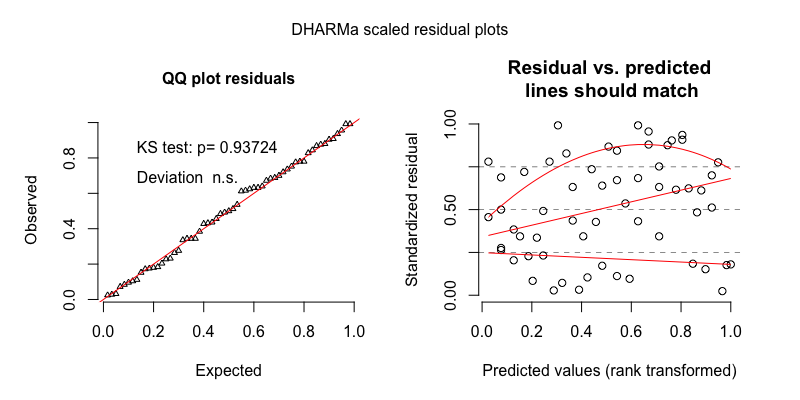
\includegraphics[width=0.9\linewidth]{www/ODS_turntaking_log_gaus_res_plot} 

}

\caption{The model residuals from the gaussian mixed-effects regression of ODS min/hr for the turn-taking sample.}\label{fig:fig12}
\end{figure}

\FloatBarrier

\subsection{Target-child-to-other turn transitions
(TC--O)}\label{models-tc_o}

\subsubsection{Random clips}\label{models-tc_o-random}

Target-child-to-other contingent response rate (TC--O transitions/min)
in the random clips demonstrated a skewed distribution with extra cases
of zero. We therefore modeled it using a zero-inflated negative binomial
mixed-effects regression.

\FloatBarrier

\begin{figure}[H]

{\centering 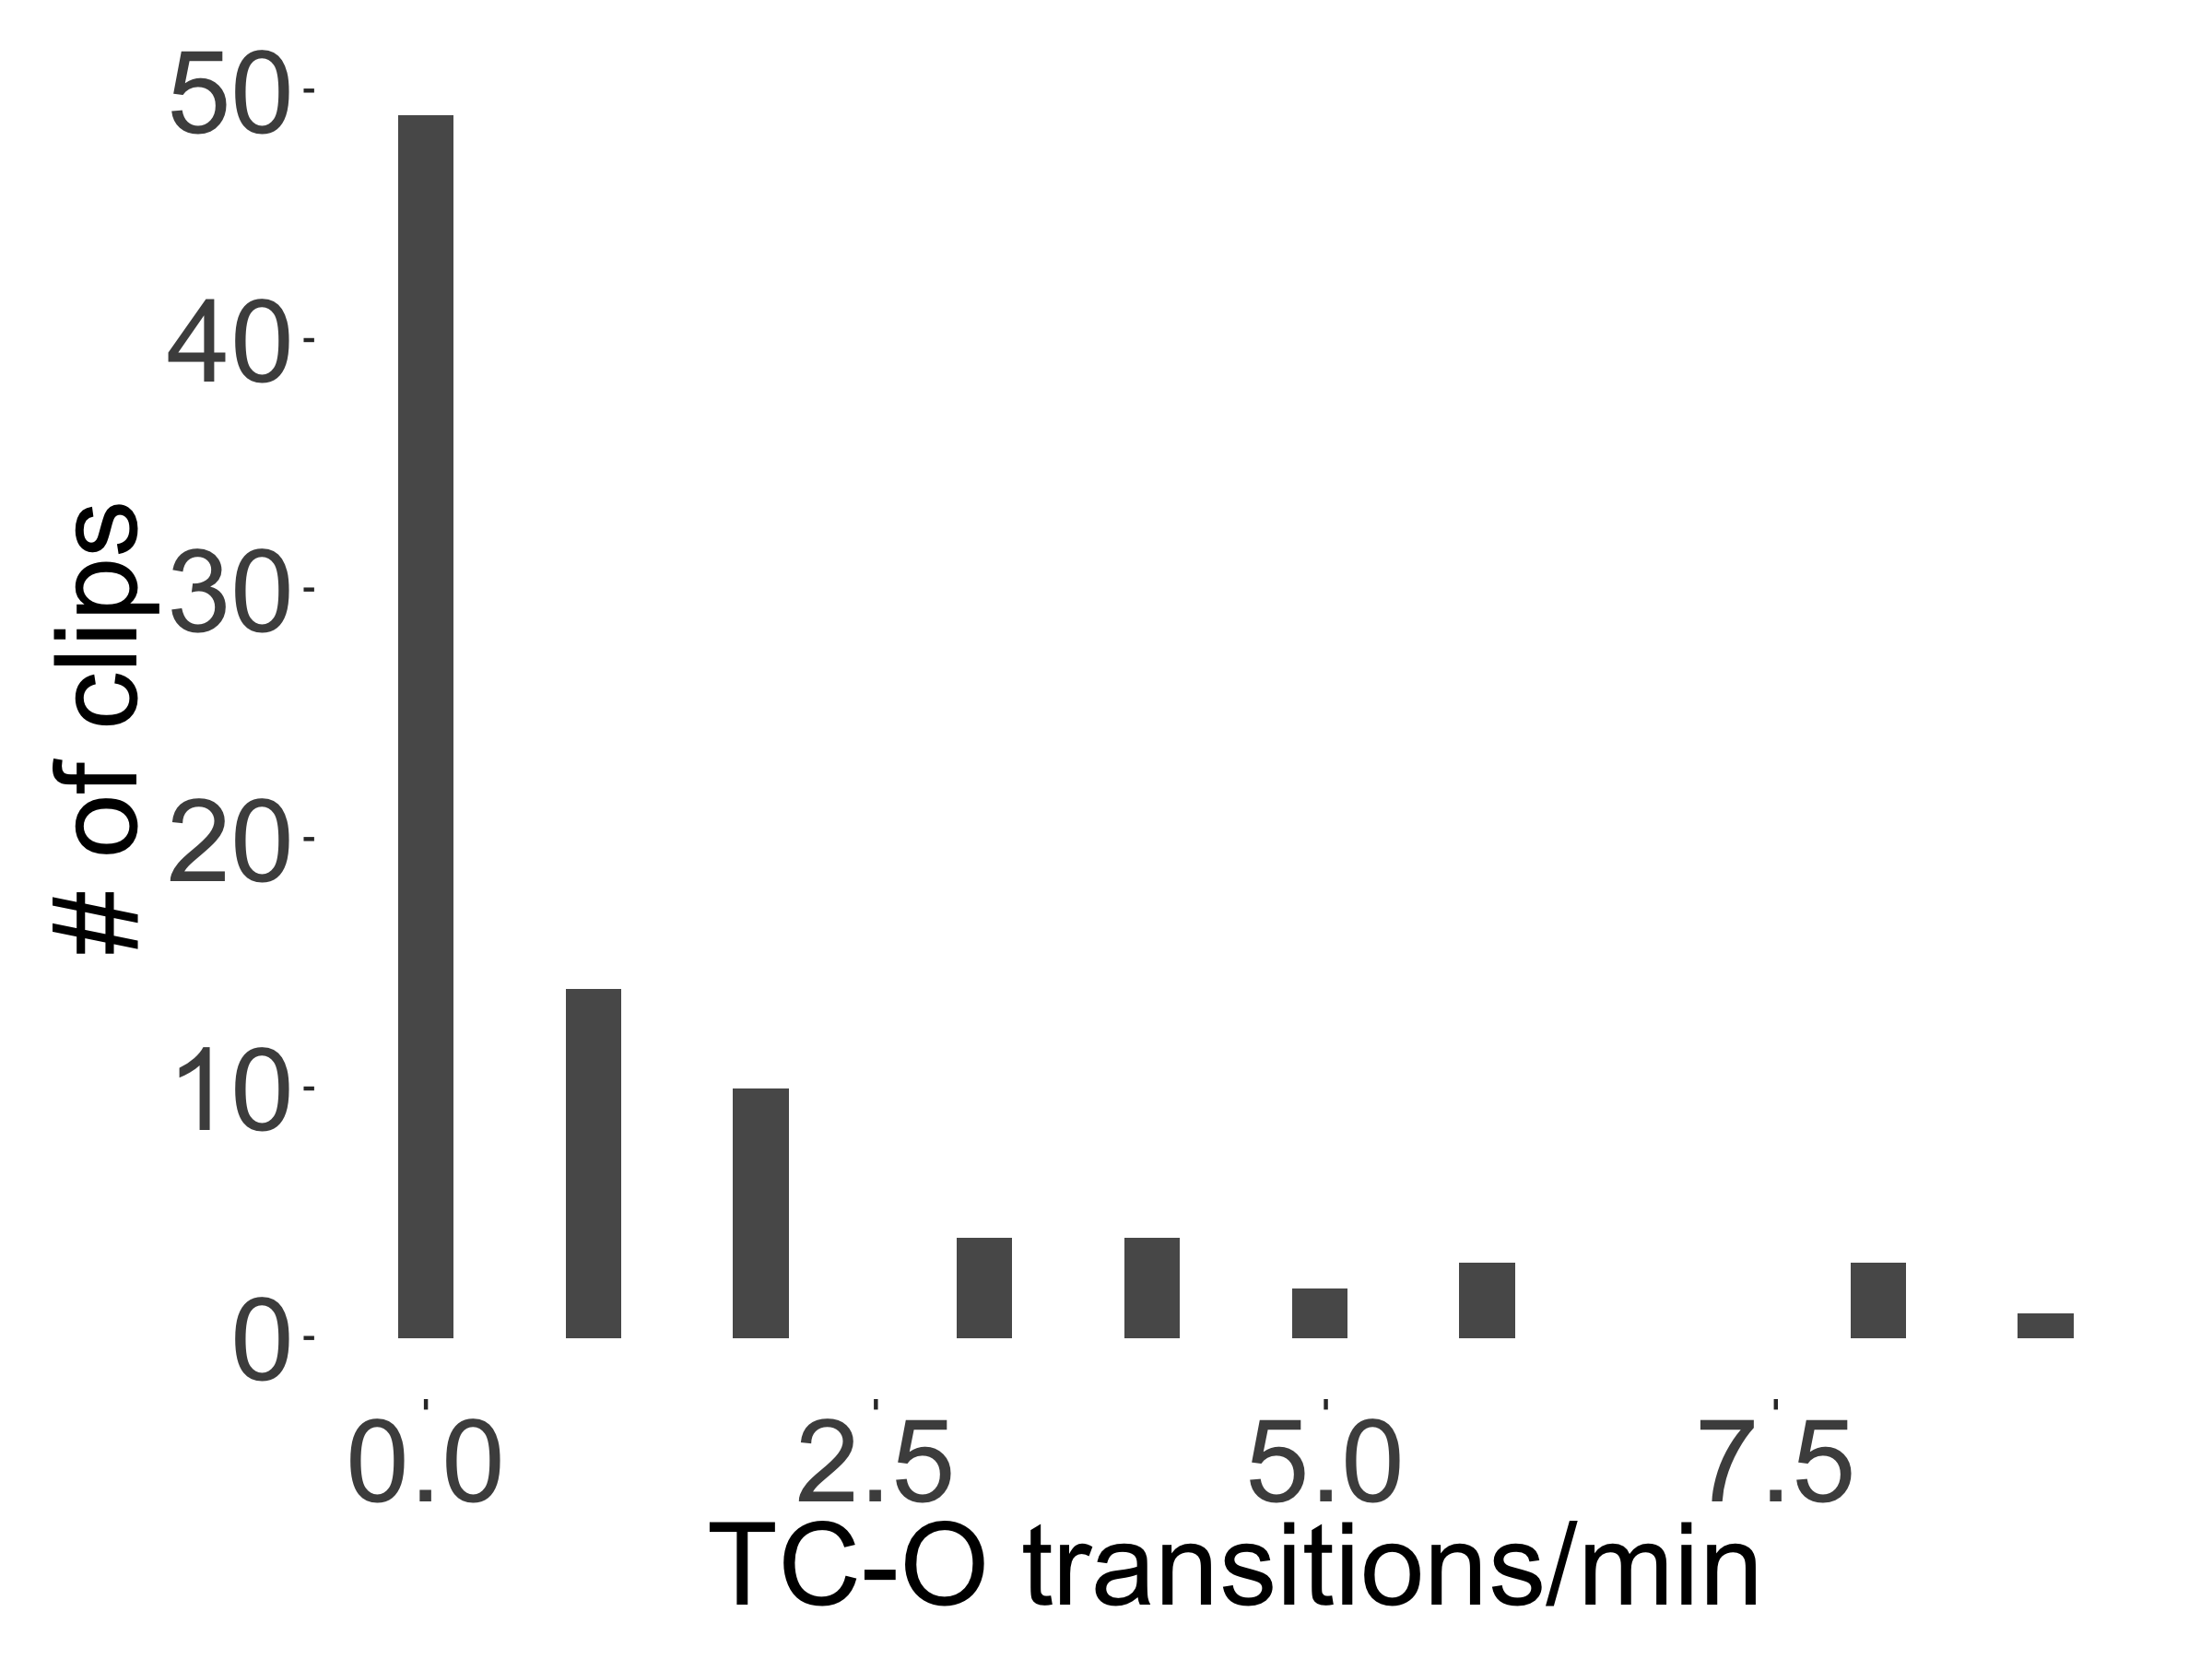
\includegraphics[width=0.4\linewidth]{www/c_o_tpm_random_distribution} 

}

\caption{The distribution of TC--O turn transitions/min rates found across the 90 random clips.}\label{fig:fig13}
\end{figure}

\FloatBarrier

\begin{table}[tbp]
\begin{center}
\begin{threeparttable}
\caption{\label{tab:tab17}Full output of the zero-inflated negative binomial mixed-effects regression of TC--O turn transitions/min for the random sample.}
\begin{tabular}{llllll}
\toprule
component & \multicolumn{1}{c}{term} & \multicolumn{1}{c}{estimate} & \multicolumn{1}{c}{std.error} & \multicolumn{1}{c}{statistic} & \multicolumn{1}{c}{p.value}\\
\midrule
cond & (Intercept) & -0.13 & 0.50 & -0.25 & 0.80\\
cond & tchiyr.std & 0.89 & 0.61 & 1.46 & 0.14\\
cond & stthr.trimorning & 0.48 & 0.45 & 1.07 & 0.28\\
cond & stthr.triafternoon & 0.34 & 0.40 & 0.85 & 0.39\\
cond & hsz.std & -0.17 & 0.45 & -0.38 & 0.70\\
cond & nsk.std & -0.18 & 0.18 & -1.01 & 0.31\\
cond & tchiyr.std:stthr.trimorning & -0.14 & 0.48 & -0.29 & 0.77\\
cond & tchiyr.std:stthr.triafternoon & -1.08 & 0.44 & -2.44 & 0.02\\
cond & tchiyr.std:hsz.std & 0.11 & 0.56 & 0.20 & 0.84\\
cond & tchiyr.std:nsk.std & 0.56 & 0.23 & 2.48 & 0.01\\
zi & (Intercept) & -116.67 & 53,056.16 & 0.00 & 1.00\\
zi & nsk.std & -100.02 & 52,343.82 & 0.00 & 1.00\\
random\_effect & aclew\_child\_id & 0.71 & NA & NA & NA\\
\bottomrule
\end{tabular}
\end{threeparttable}
\end{center}
\end{table}

\begin{table}[tbp]
\begin{center}
\begin{threeparttable}
\caption{\label{tab:tab18}Model output of the zero-inflated negative binomial mixed-effects regression of TC--O turn transitions/min for the random sample, with afternoon as the reference level for time of day.}
\begin{tabular}{llllll}
\toprule
component & \multicolumn{1}{c}{term} & \multicolumn{1}{c}{estimate} & \multicolumn{1}{c}{std.error} & \multicolumn{1}{c}{statistic} & \multicolumn{1}{c}{p.value}\\
\midrule
cond & (Intercept) & 0.22 & 0.40 & 0.54 & 0.59\\
cond & tchiyr.std & -0.20 & 0.50 & -0.40 & 0.69\\
cond & stthr.tri.amidday & -0.34 & 0.40 & -0.85 & 0.39\\
cond & stthr.tri.amorning & 0.14 & 0.32 & 0.44 & 0.66\\
cond & hsz.std & -0.17 & 0.45 & -0.38 & 0.70\\
cond & nsk.std & -0.18 & 0.18 & -1.01 & 0.31\\
cond & tchiyr.std:stthr.tri.amidday & 1.08 & 0.44 & 2.44 & 0.02\\
cond & tchiyr.std:stthr.tri.amorning & 0.94 & 0.38 & 2.52 & 0.01\\
cond & tchiyr.std:hsz.std & 0.11 & 0.56 & 0.20 & 0.84\\
cond & tchiyr.std:nsk.std & 0.56 & 0.23 & 2.48 & 0.01\\
zi & (Intercept) & -115.42 & 48,611.57 & 0.00 & 1.00\\
zi & nsk.std & -99.00 & 48,061.56 & 0.00 & 1.00\\
random\_effect & aclew\_child\_id & 0.71 & NA & NA & NA\\
\bottomrule
\end{tabular}
\end{threeparttable}
\end{center}
\end{table}

\FloatBarrier

\begin{figure}[H]

{\centering 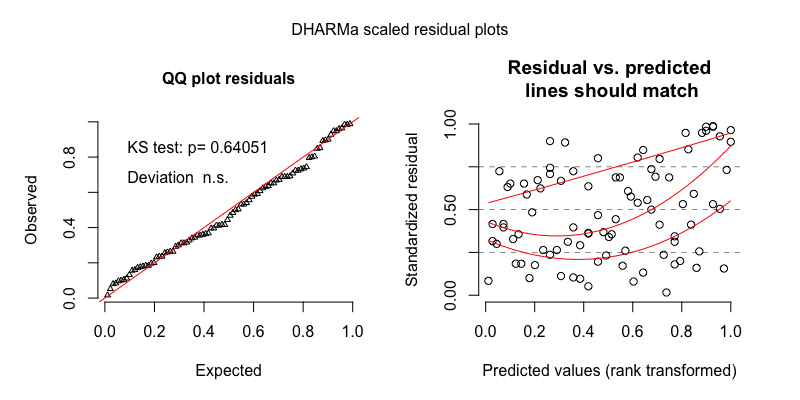
\includegraphics[width=0.9\linewidth]{www/c_o_tpm_random_z-inb_res_plot} 

}

\caption{The model residuals from the zero-inflated negative binomial mixed-effects regression of TC--O turn transitions/min for the random sample.}\label{fig:fig14}
\end{figure}

\FloatBarrier

\begin{table}[tbp]
\begin{center}
\begin{threeparttable}
\caption{\label{tab:tab19}Full output of the gaussian mixed-effects regression of TC--O turn transitions/min for the random sample, with midday as the reference level for time of day.}
\begin{tabular}{llllll}
\toprule
component & \multicolumn{1}{c}{term} & \multicolumn{1}{c}{estimate} & \multicolumn{1}{c}{std.error} & \multicolumn{1}{c}{statistic} & \multicolumn{1}{c}{p.value}\\
\midrule
cond & (Intercept) & 1.06 & 0.14 & 7.80 & 0.00\\
cond & tchiyr.std & 0.25 & 0.16 & 1.59 & 0.11\\
cond & stthr.trimorning & 0.14 & 0.12 & 1.19 & 0.24\\
cond & stthr.triafternoon & 0.01 & 0.10 & 0.13 & 0.90\\
cond & hsz.std & -0.11 & 0.14 & -0.82 & 0.41\\
cond & nsk.std & 0.09 & 0.06 & 1.56 & 0.12\\
cond & tchiyr.std:stthr.trimorning & -0.02 & 0.12 & -0.20 & 0.84\\
cond & tchiyr.std:stthr.triafternoon & -0.30 & 0.11 & -2.73 & 0.01\\
cond & tchiyr.std:hsz.std & 0.00 & 0.16 & 0.02 & 0.99\\
cond & tchiyr.std:nsk.std & 0.09 & 0.07 & 1.34 & 0.18\\
random\_effect & aclew\_child\_id & 0.21 & NA & NA & NA\\
random\_effect & Residual & 0.38 & NA & NA & NA\\
\bottomrule
\end{tabular}
\end{threeparttable}
\end{center}
\end{table}

\begin{table}[tbp]
\begin{center}
\begin{threeparttable}
\caption{\label{tab:tab20}Model output of the gaussian mixed-effects regression of TC--O turn transitions/min for the random sample, with afternoon as the reference level for time of day.}
\begin{tabular}{llllll}
\toprule
component & \multicolumn{1}{c}{term} & \multicolumn{1}{c}{estimate} & \multicolumn{1}{c}{std.error} & \multicolumn{1}{c}{statistic} & \multicolumn{1}{c}{p.value}\\
\midrule
cond & (Intercept) & 1.07 & 0.12 & 8.80 & 0.00\\
cond & tchiyr.std & -0.05 & 0.14 & -0.37 & 0.71\\
cond & stthr.tri.amidday & -0.01 & 0.10 & -0.13 & 0.90\\
cond & stthr.tri.amorning & 0.12 & 0.10 & 1.24 & 0.22\\
cond & hsz.std & -0.11 & 0.14 & -0.82 & 0.41\\
cond & nsk.std & 0.09 & 0.06 & 1.56 & 0.12\\
cond & tchiyr.std:stthr.tri.amidday & 0.30 & 0.11 & 2.73 & 0.01\\
cond & tchiyr.std:stthr.tri.amorning & 0.28 & 0.11 & 2.59 & 0.01\\
cond & tchiyr.std:hsz.std & 0.00 & 0.16 & 0.02 & 0.99\\
cond & tchiyr.std:nsk.std & 0.09 & 0.07 & 1.34 & 0.18\\
random\_effect & aclew\_child\_id & 0.21 & NA & NA & NA\\
random\_effect & Residual & 0.38 & NA & NA & NA\\
\bottomrule
\end{tabular}
\end{threeparttable}
\end{center}
\end{table}

\FloatBarrier

\begin{figure}[H]

{\centering 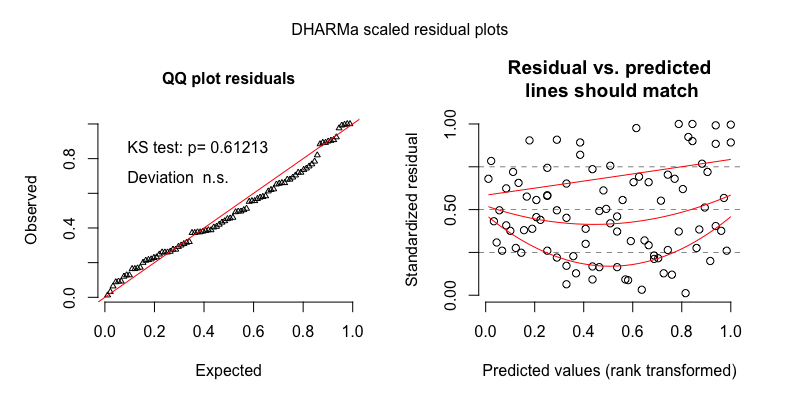
\includegraphics[width=0.9\linewidth]{www/c_o_tpm_random_log_gaus_res_plot} 

}

\caption{The model residuals from the gaussian mixed-effects regression of TC--O turn transitions/min for the random sample.}\label{fig:fig15}
\end{figure}

\FloatBarrier

\subsubsection{Turn-taking clips}\label{models-tc_o-turntaking}

TC--O transitions/min in the random clips demonstrated a fairly normal
distribution. We therefore modeled it using a plain (i.e.,
non-zero-inflated) negative binomial mixed-effects regression.

\FloatBarrier

\begin{figure}[H]

{\centering 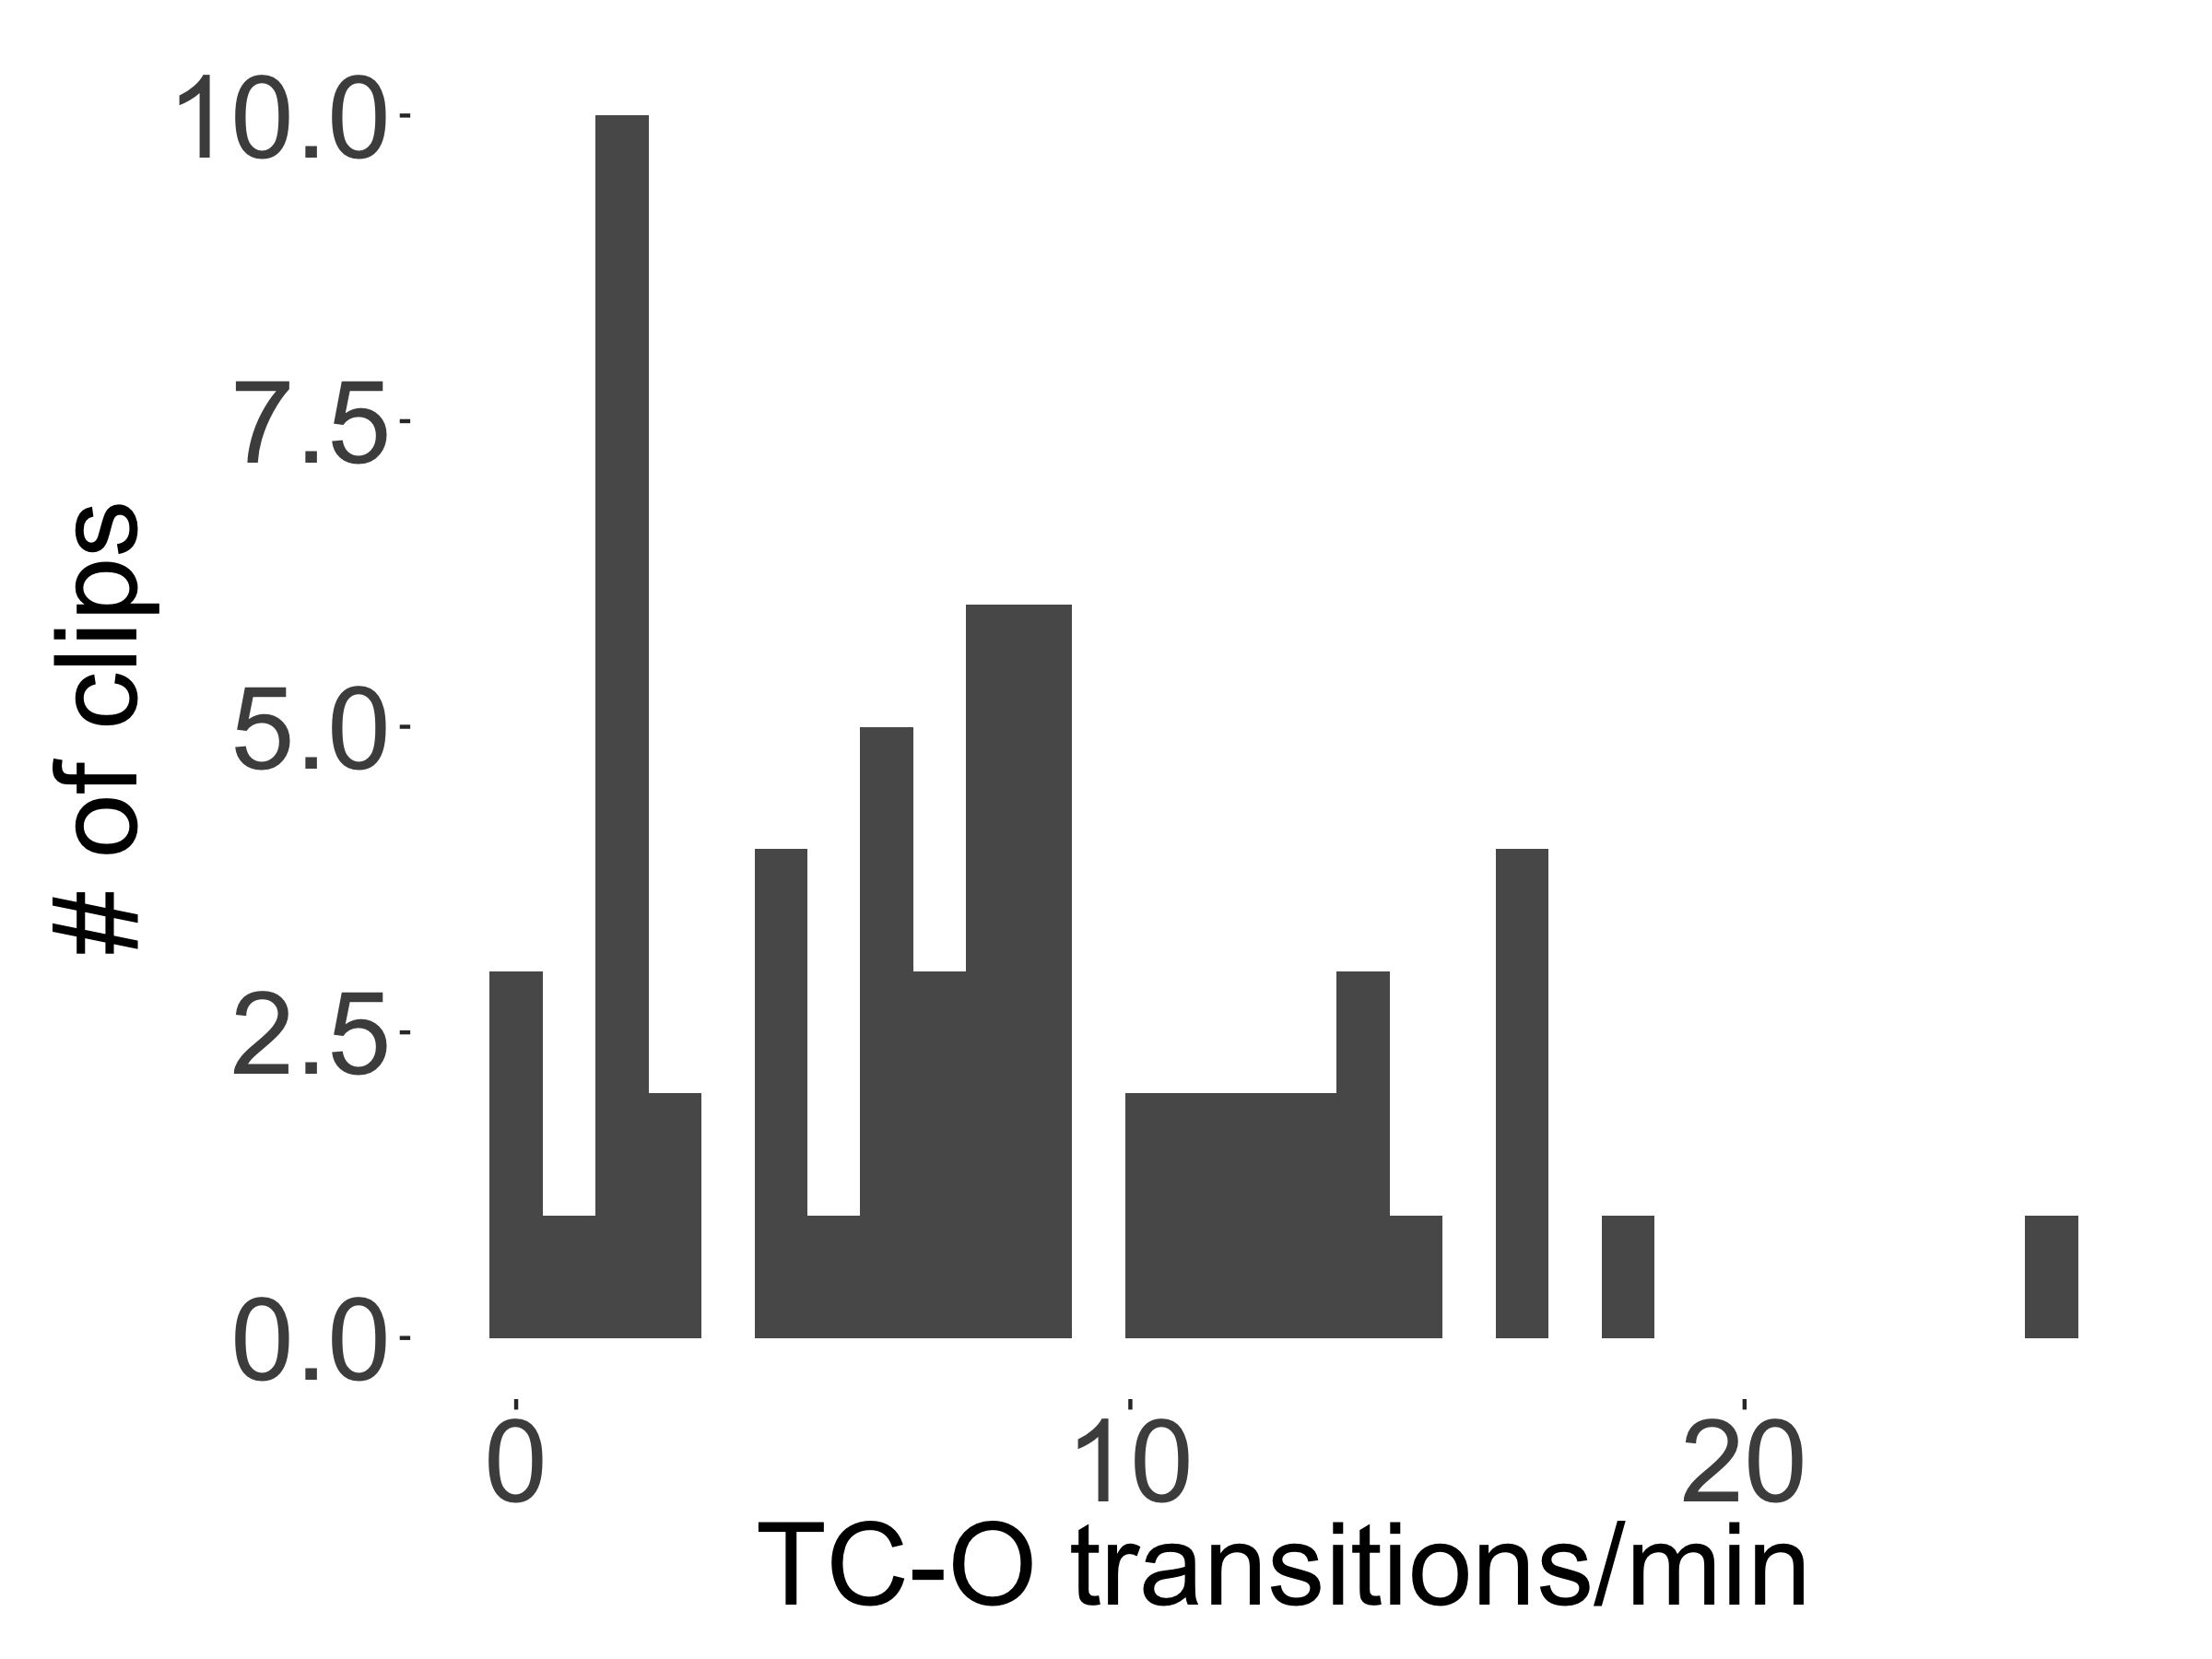
\includegraphics[width=0.4\linewidth]{www/c_o_tpm_turntaking_distribution} 

}

\caption{The distribution of TC--O turn transitions/min found across the 90 turn-taking clips.}\label{fig:fig16}
\end{figure}

\FloatBarrier

\begin{table}[tbp]
\begin{center}
\begin{threeparttable}
\caption{\label{tab:tab21}Full output of the negative binomial mixed-effects regression of TC--O turn transitions/min for the turn-taking sample.}
\begin{tabular}{llllll}
\toprule
component & \multicolumn{1}{c}{term} & \multicolumn{1}{c}{estimate} & \multicolumn{1}{c}{std.error} & \multicolumn{1}{c}{statistic} & \multicolumn{1}{c}{p.value}\\
\midrule
cond & (Intercept) & 1.78 & 0.29 & 6.19 & 0.00\\
cond & tchiyr.std & 0.12 & 0.29 & 0.40 & 0.68\\
cond & stthr.trimorning & 0.06 & 0.32 & 0.18 & 0.86\\
cond & stthr.triafternoon & 0.11 & 0.27 & 0.41 & 0.68\\
cond & hsz.std & -0.04 & 0.23 & -0.17 & 0.86\\
cond & nsk.std & -0.21 & 0.12 & -1.84 & 0.07\\
cond & tchiyr.std:stthr.trimorning & -0.04 & 0.30 & -0.13 & 0.89\\
cond & tchiyr.std:stthr.triafternoon & -0.19 & 0.25 & -0.75 & 0.45\\
cond & tchiyr.std:hsz.std & -0.19 & 0.28 & -0.68 & 0.50\\
cond & tchiyr.std:nsk.std & 0.05 & 0.13 & 0.41 & 0.68\\
random\_effect & aclew\_child\_id & 0.32 & NA & NA & NA\\
\bottomrule
\end{tabular}
\end{threeparttable}
\end{center}
\end{table}

\begin{table}[tbp]
\begin{center}
\begin{threeparttable}
\caption{\label{tab:tab22}Model output of the negative binomial mixed-effects regression of TC--O turn transitions/min for the turn-taking sample, with afternoon as the reference level for time of day.}
\begin{tabular}{llllll}
\toprule
component & \multicolumn{1}{c}{term} & \multicolumn{1}{c}{estimate} & \multicolumn{1}{c}{std.error} & \multicolumn{1}{c}{statistic} & \multicolumn{1}{c}{p.value}\\
\midrule
cond & (Intercept) & 1.90 & 0.24 & 7.88 & 0.00\\
cond & tchiyr.std & -0.07 & 0.27 & -0.26 & 0.79\\
cond & stthr.tri.amidday & -0.11 & 0.27 & -0.41 & 0.68\\
cond & stthr.tri.amorning & -0.05 & 0.24 & -0.21 & 0.83\\
cond & hsz.std & -0.04 & 0.23 & -0.17 & 0.86\\
cond & nsk.std & -0.21 & 0.12 & -1.84 & 0.07\\
cond & tchiyr.std:stthr.tri.amidday & 0.19 & 0.25 & 0.75 & 0.45\\
cond & tchiyr.std:stthr.tri.amorning & 0.15 & 0.27 & 0.56 & 0.58\\
cond & tchiyr.std:hsz.std & -0.19 & 0.28 & -0.68 & 0.50\\
cond & tchiyr.std:nsk.std & 0.05 & 0.13 & 0.41 & 0.68\\
random\_effect & aclew\_child\_id & 0.32 & NA & NA & NA\\
\bottomrule
\end{tabular}
\end{threeparttable}
\end{center}
\end{table}

\FloatBarrier

\begin{figure}[H]

{\centering 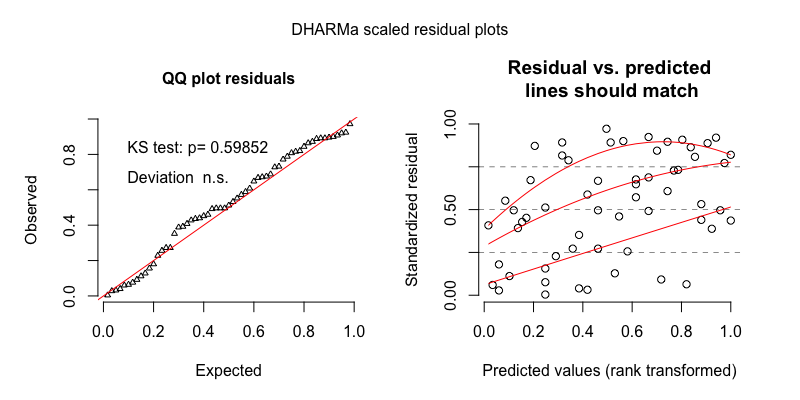
\includegraphics[width=0.9\linewidth]{www/c_o_tpm_turntaking_nb_res_plot} 

}

\caption{The model residuals from the zero-inflated negative binomial mixed-effects regression of TC--O turn transitions/min for the turn-taking sample.}\label{fig:fig17}
\end{figure}

\FloatBarrier

\begin{table}[tbp]
\begin{center}
\begin{threeparttable}
\caption{\label{tab:tab23}Full output of the gaussian mixed-effects regression of TC--O turn transitions/min for the turn-taking sample, with midday as the reference level for time of day.}
\begin{tabular}{llllll}
\toprule
component & \multicolumn{1}{c}{term} & \multicolumn{1}{c}{estimate} & \multicolumn{1}{c}{std.error} & \multicolumn{1}{c}{statistic} & \multicolumn{1}{c}{p.value}\\
\midrule
cond & (Intercept) & 2.07 & 0.20 & 10.19 & 0.00\\
cond & tchiyr.std & -0.02 & 0.23 & -0.09 & 0.93\\
cond & stthr.tri.amidday & -0.11 & 0.21 & -0.52 & 0.60\\
cond & stthr.tri.amorning & -0.08 & 0.20 & -0.40 & 0.69\\
cond & hsz.std & -0.02 & 0.20 & -0.12 & 0.90\\
cond & nsk.std & -0.18 & 0.10 & -1.86 & 0.06\\
cond & tchiyr.std:stthr.tri.amidday & 0.11 & 0.20 & 0.55 & 0.58\\
cond & tchiyr.std:stthr.tri.amorning & 0.09 & 0.22 & 0.42 & 0.67\\
cond & tchiyr.std:hsz.std & -0.17 & 0.25 & -0.68 & 0.50\\
cond & tchiyr.std:nsk.std & 0.09 & 0.12 & 0.79 & 0.43\\
random\_effect & aclew\_child\_id & 0.30 & NA & NA & NA\\
random\_effect & Residual & 0.51 & NA & NA & NA\\
\bottomrule
\end{tabular}
\end{threeparttable}
\end{center}
\end{table}

\begin{table}[tbp]
\begin{center}
\begin{threeparttable}
\caption{\label{tab:tab24}Model output of the gaussian mixed-effects regression of TC--O turn transitions/min for the turn-taking sample, with afternoon as the reference level for time of day.}
\begin{tabular}{llllll}
\toprule
component & \multicolumn{1}{c}{term} & \multicolumn{1}{c}{estimate} & \multicolumn{1}{c}{std.error} & \multicolumn{1}{c}{statistic} & \multicolumn{1}{c}{p.value}\\
\midrule
cond & (Intercept) & 2.07 & 0.20 & 10.19 & 0.00\\
cond & tchiyr.std & -0.02 & 0.23 & -0.09 & 0.93\\
cond & stthr.tri.amidday & -0.11 & 0.21 & -0.52 & 0.60\\
cond & stthr.tri.amorning & -0.08 & 0.20 & -0.40 & 0.69\\
cond & hsz.std & -0.02 & 0.20 & -0.12 & 0.90\\
cond & nsk.std & -0.18 & 0.10 & -1.86 & 0.06\\
cond & tchiyr.std:stthr.tri.amidday & 0.11 & 0.20 & 0.55 & 0.58\\
cond & tchiyr.std:stthr.tri.amorning & 0.09 & 0.22 & 0.42 & 0.67\\
cond & tchiyr.std:hsz.std & -0.17 & 0.25 & -0.68 & 0.50\\
cond & tchiyr.std:nsk.std & 0.09 & 0.12 & 0.79 & 0.43\\
random\_effect & aclew\_child\_id & 0.30 & NA & NA & NA\\
random\_effect & Residual & 0.51 & NA & NA & NA\\
\bottomrule
\end{tabular}
\end{threeparttable}
\end{center}
\end{table}

\FloatBarrier

\begin{figure}[H]

{\centering 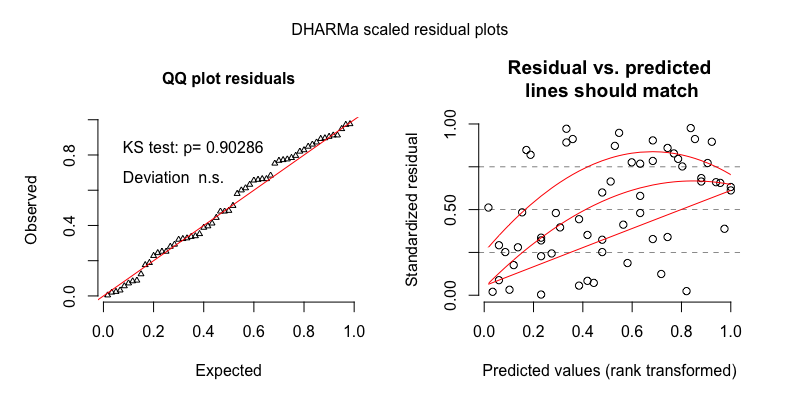
\includegraphics[width=0.9\linewidth]{www/c_o_tpm_turntaking_log_gaus_res_plot} 

}

\caption{The model residuals from the gaussian mixed-effects regression of TC--O turn transitions/min for the turn-taking sample.}\label{fig:fig18}
\end{figure}

\FloatBarrier

\subsection{Other-to-target-child turn transitions
(O--TC)}\label{models-o_tc}

\subsubsection{Random clips}\label{models-o_tc-random}

Other-to-target-child contingent response rate (O--TC transitions/min)
in the random clips demonstrated a skewed distribution with extra cases
of zero. We therefore modeled it using a zero-inflated negative binomial
mixed-effects regression.

\FloatBarrier

\begin{figure}[H]

{\centering 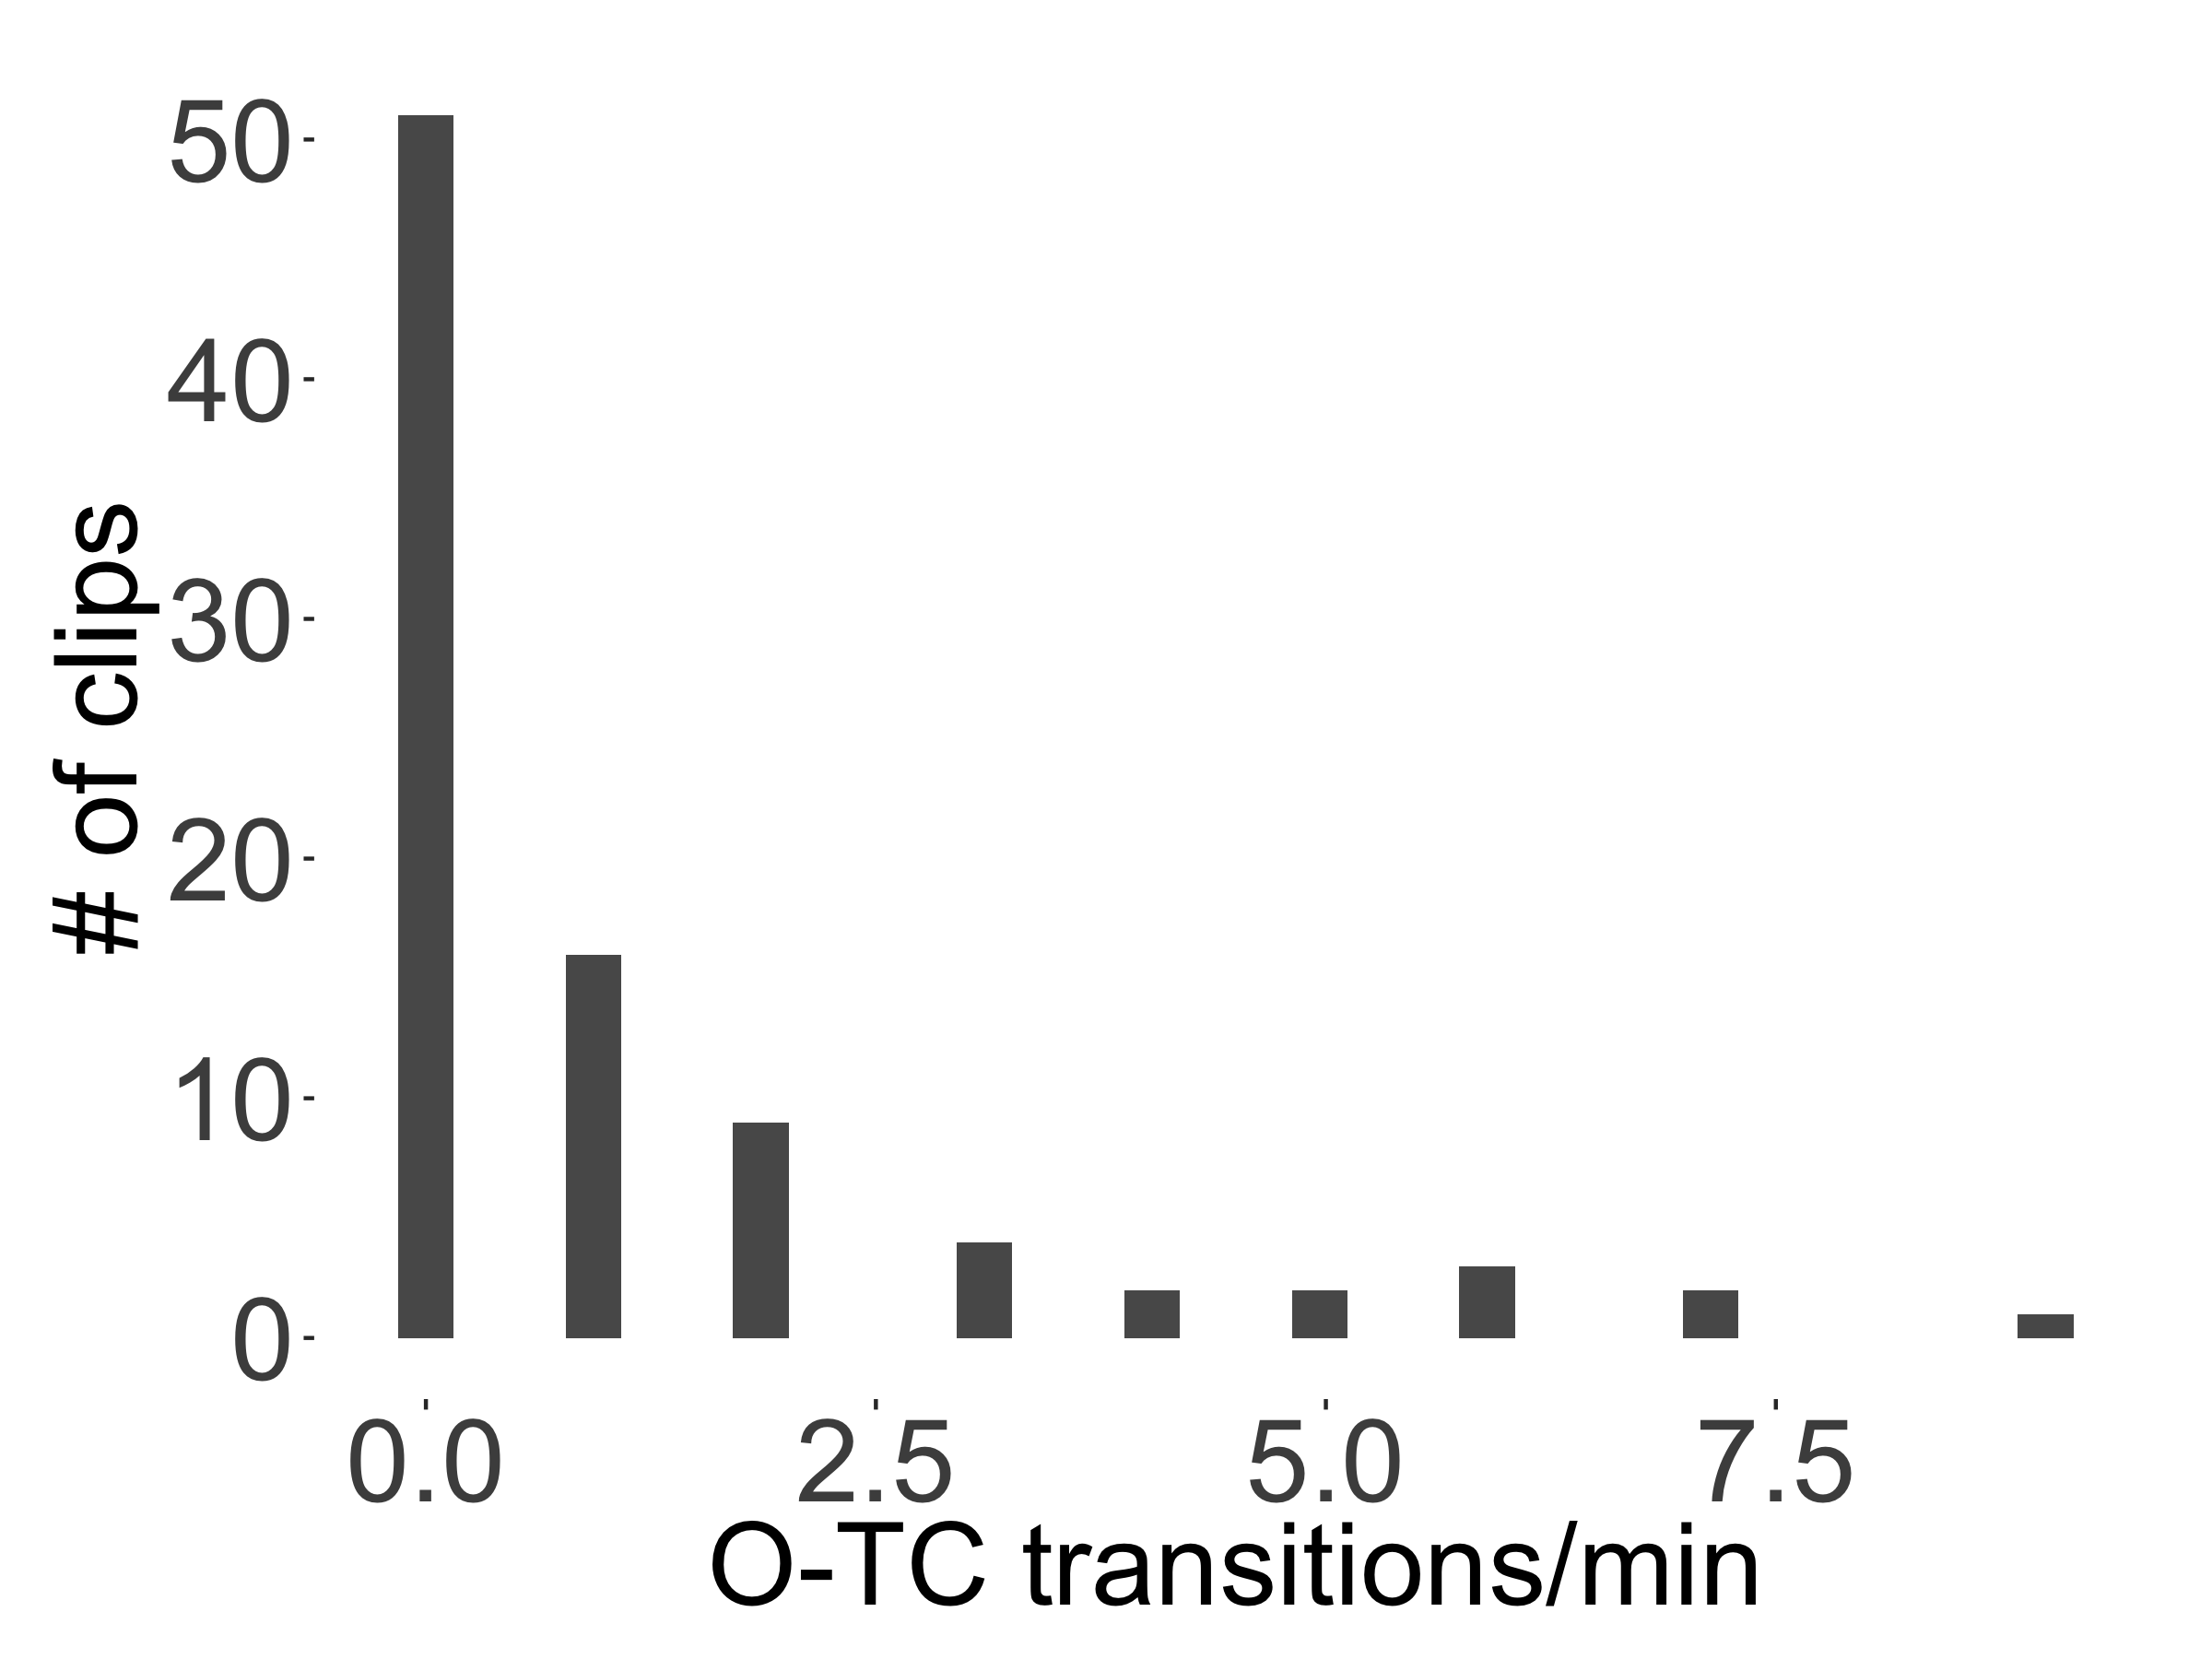
\includegraphics[width=0.4\linewidth]{www/o_c_tpm_random_distribution} 

}

\caption{The distribution of O--TC turn transitions/min rates found across the 90 random clips.}\label{fig:fig19}
\end{figure}

\FloatBarrier

\begin{table}[tbp]
\begin{center}
\begin{threeparttable}
\caption{\label{tab:tab25}Full output of the zero-inflated negative binomial mixed-effects regression of O--TCturn transitions/min for the random sample, with midday as the reference level for time of day.}
\begin{tabular}{llllll}
\toprule
component & \multicolumn{1}{c}{term} & \multicolumn{1}{c}{estimate} & \multicolumn{1}{c}{std.error} & \multicolumn{1}{c}{statistic} & \multicolumn{1}{c}{p.value}\\
\midrule
cond & (Intercept) & -0.46 & 0.54 & -0.84 & 0.40\\
cond & tchiyr.std & 1.14 & 0.66 & 1.74 & 0.08\\
cond & stthr.trimorning & 0.32 & 0.49 & 0.65 & 0.52\\
cond & stthr.triafternoon & 0.50 & 0.41 & 1.21 & 0.22\\
cond & hsz.std & -0.20 & 0.50 & -0.41 & 0.68\\
cond & nsk.std & -0.14 & 0.18 & -0.79 & 0.43\\
cond & tchiyr.std:stthr.trimorning & -0.12 & 0.51 & -0.24 & 0.81\\
cond & tchiyr.std:stthr.triafternoon & -1.46 & 0.46 & -3.13 & 0.00\\
cond & tchiyr.std:hsz.std & 0.14 & 0.61 & 0.23 & 0.82\\
cond & tchiyr.std:nsk.std & 0.52 & 0.22 & 2.30 & 0.02\\
zi & (Intercept) & -115.46 & 43,943.60 & 0.00 & 1.00\\
zi & nsk.std & -98.63 & 42,142.48 & 0.00 & 1.00\\
random\_effect & aclew\_child\_id & 0.80 & NA & NA & NA\\
\bottomrule
\end{tabular}
\end{threeparttable}
\end{center}
\end{table}

\begin{table}[tbp]
\begin{center}
\begin{threeparttable}
\caption{\label{tab:tab26}Model output of the zero-inflated negative binomial mixed-effects regression of O--TC turn transitions/min for the random sample, with afternoon as the reference level for time of day.}
\begin{tabular}{llllll}
\toprule
component & \multicolumn{1}{c}{term} & \multicolumn{1}{c}{estimate} & \multicolumn{1}{c}{std.error} & \multicolumn{1}{c}{statistic} & \multicolumn{1}{c}{p.value}\\
\midrule
cond & (Intercept) & 0.04 & 0.43 & 0.08 & 0.93\\
cond & tchiyr.std & -0.32 & 0.54 & -0.59 & 0.56\\
cond & stthr.tri.amidday & -0.50 & 0.41 & -1.21 & 0.22\\
cond & stthr.tri.amorning & -0.18 & 0.36 & -0.49 & 0.62\\
cond & hsz.std & -0.20 & 0.50 & -0.41 & 0.68\\
cond & nsk.std & -0.14 & 0.18 & -0.79 & 0.43\\
cond & tchiyr.std:stthr.tri.amidday & 1.46 & 0.46 & 3.13 & 0.00\\
cond & tchiyr.std:stthr.tri.amorning & 1.33 & 0.42 & 3.19 & 0.00\\
cond & tchiyr.std:hsz.std & 0.14 & 0.61 & 0.23 & 0.82\\
cond & tchiyr.std:nsk.std & 0.52 & 0.22 & 2.30 & 0.02\\
zi & (Intercept) & -115.66 & 41,463.41 & 0.00 & 1.00\\
zi & nsk.std & -98.60 & 38,727.01 & 0.00 & 1.00\\
random\_effect & aclew\_child\_id & 0.80 & NA & NA & NA\\
\bottomrule
\end{tabular}
\end{threeparttable}
\end{center}
\end{table}

\FloatBarrier

\begin{figure}[H]

{\centering 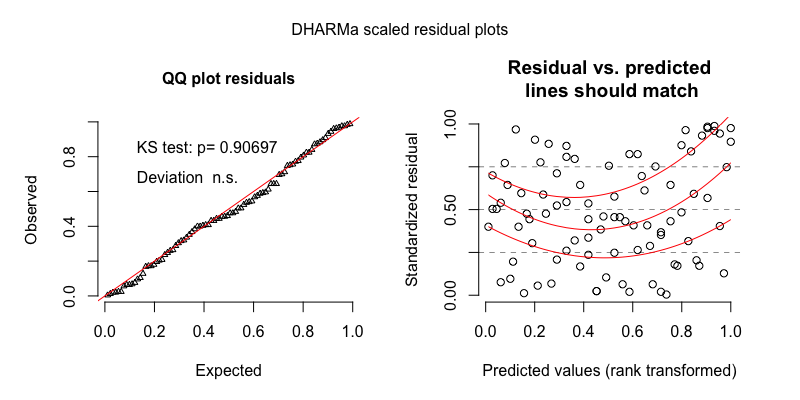
\includegraphics[width=0.9\linewidth]{www/o_c_tpm_random_z-inb_res_plot} 

}

\caption{The model residuals from the zero-inflated negative binomial mixed-effects regression of O--TC turn transitions/min for the random sample.}\label{fig:fig20}
\end{figure}

\FloatBarrier

\begin{table}[tbp]
\begin{center}
\begin{threeparttable}
\caption{\label{tab:tab27}Full output of the gaussian mixed-effects regression of O--TC turn transitions/min for the random sample, with midday as the reference level for time of day.}
\begin{tabular}{llllll}
\toprule
component & \multicolumn{1}{c}{term} & \multicolumn{1}{c}{estimate} & \multicolumn{1}{c}{std.error} & \multicolumn{1}{c}{statistic} & \multicolumn{1}{c}{p.value}\\
\midrule
cond & (Intercept) & 1.01 & 0.12 & 8.09 & 0.00\\
cond & tchiyr.std & 0.23 & 0.14 & 1.57 & 0.12\\
cond & stthr.trimorning & 0.10 & 0.11 & 0.92 & 0.36\\
cond & stthr.triafternoon & 0.00 & 0.10 & 0.00 & 1.00\\
cond & hsz.std & -0.12 & 0.12 & -0.96 & 0.34\\
cond & nsk.std & 0.07 & 0.05 & 1.33 & 0.18\\
cond & tchiyr.std:stthr.trimorning & -0.02 & 0.12 & -0.17 & 0.87\\
cond & tchiyr.std:stthr.triafternoon & -0.29 & 0.10 & -2.76 & 0.01\\
cond & tchiyr.std:hsz.std & -0.03 & 0.15 & -0.19 & 0.85\\
cond & tchiyr.std:nsk.std & 0.08 & 0.07 & 1.13 & 0.26\\
random\_effect & aclew\_child\_id & 0.19 & NA & NA & NA\\
random\_effect & Residual & 0.36 & NA & NA & NA\\
\bottomrule
\end{tabular}
\end{threeparttable}
\end{center}
\end{table}

\begin{table}[tbp]
\begin{center}
\begin{threeparttable}
\caption{\label{tab:tab28}Model output of the gaussian mixed-effects regression of O--TC turn transitions/min for the random sample, with afternoon as the reference level for time of day.}
\begin{tabular}{llllll}
\toprule
component & \multicolumn{1}{c}{term} & \multicolumn{1}{c}{estimate} & \multicolumn{1}{c}{std.error} & \multicolumn{1}{c}{statistic} & \multicolumn{1}{c}{p.value}\\
\midrule
cond & (Intercept) & 1.01 & 0.11 & 9.04 & 0.00\\
cond & tchiyr.std & -0.06 & 0.13 & -0.45 & 0.66\\
cond & stthr.tri.amidday & 0.00 & 0.10 & 0.00 & 1.00\\
cond & stthr.tri.amorning & 0.10 & 0.09 & 1.06 & 0.29\\
cond & hsz.std & -0.12 & 0.12 & -0.96 & 0.34\\
cond & nsk.std & 0.07 & 0.05 & 1.33 & 0.18\\
cond & tchiyr.std:stthr.tri.amidday & 0.29 & 0.10 & 2.76 & 0.01\\
cond & tchiyr.std:stthr.tri.amorning & 0.27 & 0.10 & 2.66 & 0.01\\
cond & tchiyr.std:hsz.std & -0.03 & 0.15 & -0.19 & 0.85\\
cond & tchiyr.std:nsk.std & 0.08 & 0.07 & 1.13 & 0.26\\
random\_effect & aclew\_child\_id & 0.19 & NA & NA & NA\\
random\_effect & Residual & 0.36 & NA & NA & NA\\
\bottomrule
\end{tabular}
\end{threeparttable}
\end{center}
\end{table}

\FloatBarrier

\begin{figure}[H]

{\centering 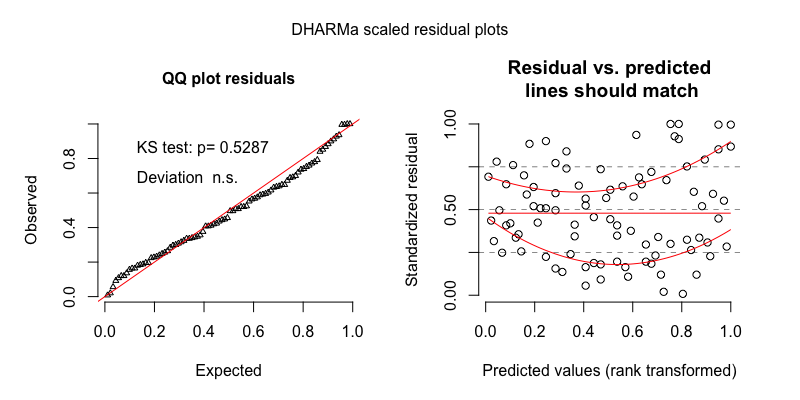
\includegraphics[width=0.9\linewidth]{www/o_c_tpm_random_log_gaus_res_plot} 

}

\caption{The model residuals from the gaussian mixed-effects regression of O--TC turn transitions/min for the random sample.}\label{fig:fig21}
\end{figure}

\FloatBarrier

\subsubsection{Turn-taking clips}\label{models-o_tc-turntaking}

O--TC transitions/min in the random clips demonstrated a fairly normal
distribution. We therefore modeled it using a plain (i.e.,
non-zero-inflated) negative binomial mixed-effects regression.

\FloatBarrier

\begin{figure}[H]

{\centering 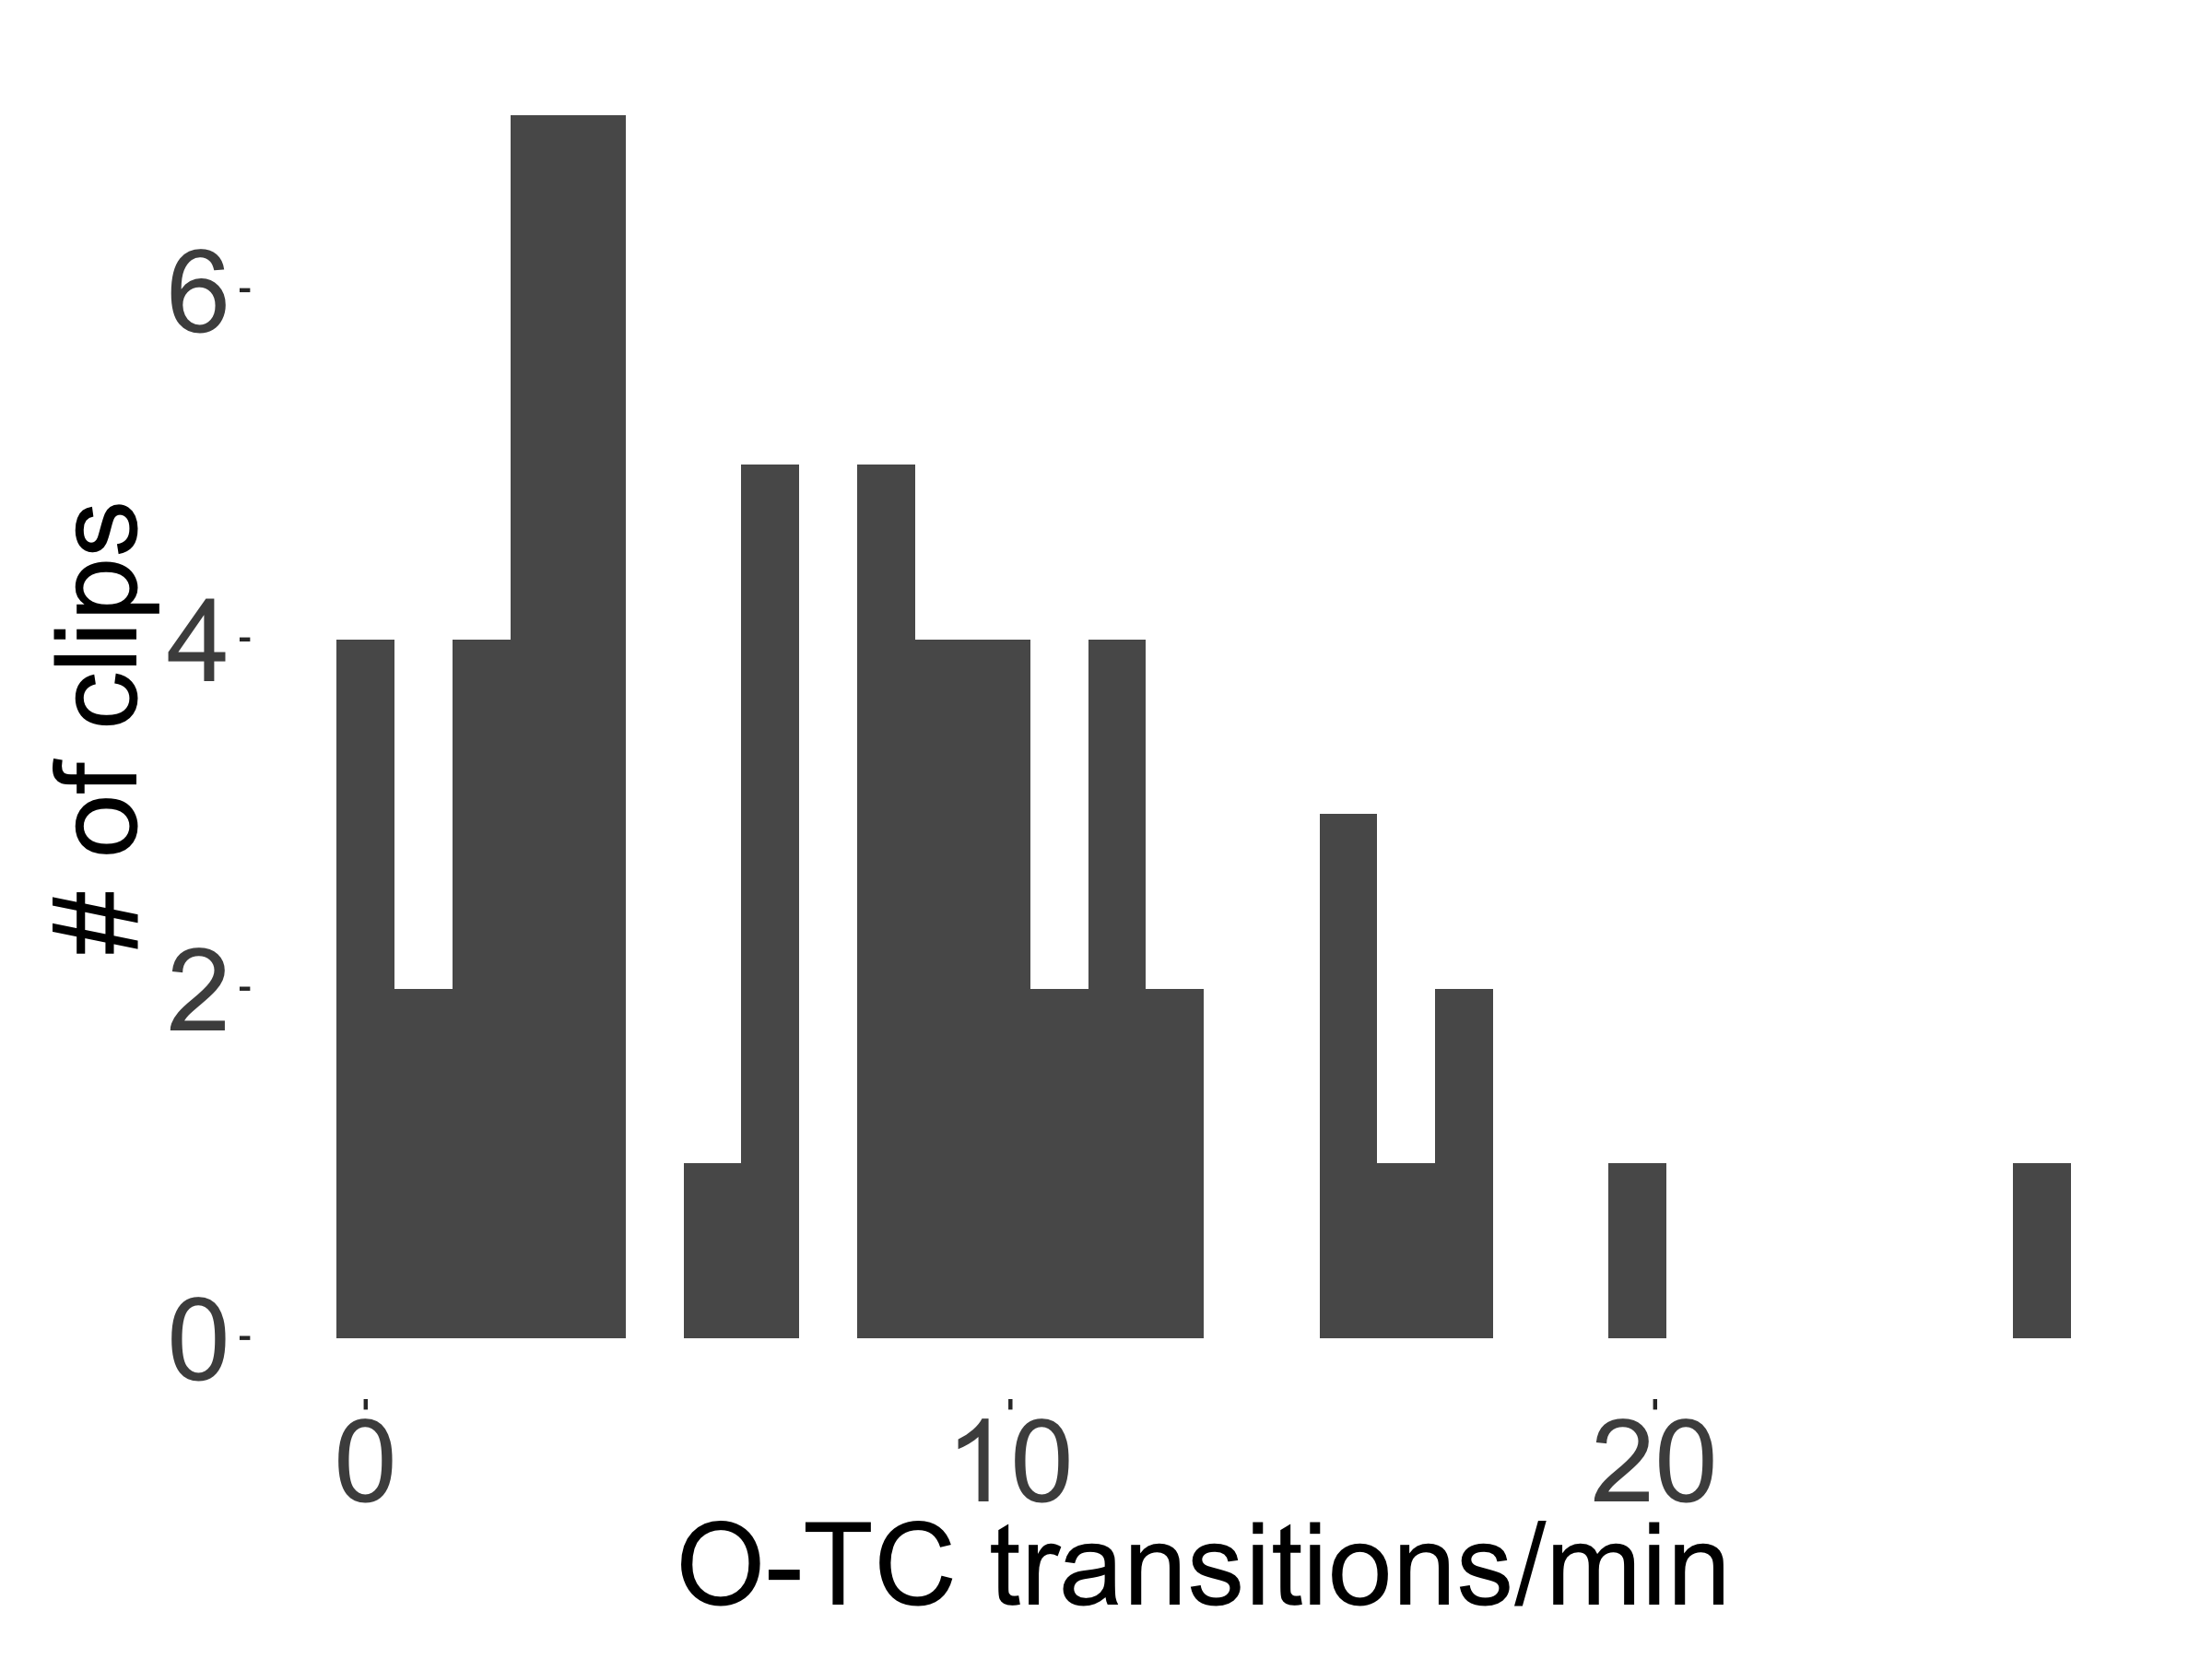
\includegraphics[width=0.4\linewidth]{www/o_c_tpm_turntaking_distribution} 

}

\caption{The distribution of O--TC turn transitions/min found across the 90 turn-taking clips.}\label{fig:fig22}
\end{figure}

\FloatBarrier

\begin{table}[tbp]
\begin{center}
\begin{threeparttable}
\caption{\label{tab:tab29}Full output of the negative binomial mixed-effects regression of O--TC turn transitions/min for the turn-taking sample.}
\begin{tabular}{llllll}
\toprule
component & \multicolumn{1}{c}{term} & \multicolumn{1}{c}{estimate} & \multicolumn{1}{c}{std.error} & \multicolumn{1}{c}{statistic} & \multicolumn{1}{c}{p.value}\\
\midrule
cond & (Intercept) & 1.84 & 0.29 & 6.32 & 0.00\\
cond & tchiyr.std & 0.06 & 0.30 & 0.20 & 0.84\\
cond & stthr.trimorning & -0.05 & 0.33 & -0.15 & 0.88\\
cond & stthr.triafternoon & 0.03 & 0.28 & 0.10 & 0.92\\
cond & hsz.std & -0.04 & 0.23 & -0.16 & 0.88\\
cond & nsk.std & -0.23 & 0.12 & -1.88 & 0.06\\
cond & tchiyr.std:stthr.trimorning & 0.12 & 0.31 & 0.39 & 0.69\\
cond & tchiyr.std:stthr.triafternoon & -0.08 & 0.26 & -0.30 & 0.77\\
cond & tchiyr.std:hsz.std & -0.19 & 0.28 & -0.66 & 0.51\\
cond & tchiyr.std:nsk.std & 0.08 & 0.14 & 0.62 & 0.53\\
random\_effect & aclew\_child\_id & 0.31 & NA & NA & NA\\
\bottomrule
\end{tabular}
\end{threeparttable}
\end{center}
\end{table}

\begin{table}[tbp]
\begin{center}
\begin{threeparttable}
\caption{\label{tab:tab30}Model output of the negative binomial mixed-effects regression of O--TC turn transitions/min for the turn-taking sample, with afternoon as the reference level for time of day.}
\begin{tabular}{llllll}
\toprule
component & \multicolumn{1}{c}{term} & \multicolumn{1}{c}{estimate} & \multicolumn{1}{c}{std.error} & \multicolumn{1}{c}{statistic} & \multicolumn{1}{c}{p.value}\\
\midrule
cond & (Intercept) & 1.87 & 0.25 & 7.55 & 0.00\\
cond & tchiyr.std & -0.02 & 0.27 & -0.06 & 0.95\\
cond & stthr.tri.amidday & -0.03 & 0.28 & -0.10 & 0.92\\
cond & stthr.tri.amorning & -0.08 & 0.26 & -0.30 & 0.77\\
cond & hsz.std & -0.04 & 0.23 & -0.16 & 0.88\\
cond & nsk.std & -0.23 & 0.12 & -1.88 & 0.06\\
cond & tchiyr.std:stthr.tri.amidday & 0.08 & 0.26 & 0.30 & 0.77\\
cond & tchiyr.std:stthr.tri.amorning & 0.20 & 0.27 & 0.73 & 0.46\\
cond & tchiyr.std:hsz.std & -0.19 & 0.28 & -0.66 & 0.51\\
cond & tchiyr.std:nsk.std & 0.08 & 0.14 & 0.62 & 0.53\\
random\_effect & aclew\_child\_id & 0.31 & NA & NA & NA\\
\bottomrule
\end{tabular}
\end{threeparttable}
\end{center}
\end{table}

\FloatBarrier

\begin{figure}[H]

{\centering 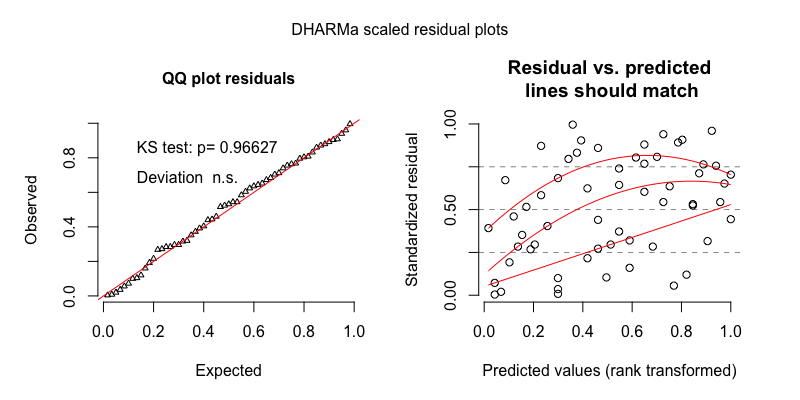
\includegraphics[width=0.9\linewidth]{www/o_c_tpm_turntaking_nb_res_plot} 

}

\caption{The model residuals from the negative binomial mixed-effects regression of O--TC turn transitions/min for the turn-taking sample.}\label{fig:fig23}
\end{figure}

\FloatBarrier

\begin{table}[tbp]
\begin{center}
\begin{threeparttable}
\caption{\label{tab:tab31}Full output of the gaussian mixed-effects regression of O--TC turn transitions/min for the turn-taking sample, with midday as the reference level for time of day.}
\begin{tabular}{llllll}
\toprule
component & \multicolumn{1}{c}{term} & \multicolumn{1}{c}{estimate} & \multicolumn{1}{c}{std.error} & \multicolumn{1}{c}{statistic} & \multicolumn{1}{c}{p.value}\\
\midrule
cond & (Intercept) & 2.01 & 0.25 & 8.10 & 0.00\\
cond & tchiyr.std & 0.04 & 0.25 & 0.16 & 0.87\\
cond & stthr.trimorning & -0.09 & 0.27 & -0.34 & 0.74\\
cond & stthr.triafternoon & 0.04 & 0.22 & 0.16 & 0.87\\
cond & hsz.std & 0.00 & 0.21 & -0.01 & 0.99\\
cond & nsk.std & -0.20 & 0.10 & -1.98 & 0.05\\
cond & tchiyr.std:stthr.trimorning & 0.17 & 0.25 & 0.66 & 0.51\\
cond & tchiyr.std:stthr.triafternoon & 0.00 & 0.21 & -0.02 & 0.99\\
cond & tchiyr.std:hsz.std & -0.13 & 0.26 & -0.52 & 0.61\\
cond & tchiyr.std:nsk.std & 0.08 & 0.12 & 0.69 & 0.49\\
random\_effect & aclew\_child\_id & 0.30 & NA & NA & NA\\
random\_effect & Residual & 0.53 & NA & NA & NA\\
\bottomrule
\end{tabular}
\end{threeparttable}
\end{center}
\end{table}

\begin{table}[tbp]
\begin{center}
\begin{threeparttable}
\caption{\label{tab:tab32}Model output of the gaussian mixed-effects regression of O--TC turn transitions/min for the turn-taking sample, with afternoon as the reference level for time of day.}
\begin{tabular}{llllll}
\toprule
component & \multicolumn{1}{c}{term} & \multicolumn{1}{c}{estimate} & \multicolumn{1}{c}{std.error} & \multicolumn{1}{c}{statistic} & \multicolumn{1}{c}{p.value}\\
\midrule
cond & (Intercept) & 2.04 & 0.21 & 9.74 & 0.00\\
cond & tchiyr.std & 0.04 & 0.24 & 0.15 & 0.88\\
cond & stthr.tri.amidday & -0.04 & 0.22 & -0.16 & 0.87\\
cond & stthr.tri.amorning & -0.13 & 0.22 & -0.59 & 0.56\\
cond & hsz.std & 0.00 & 0.21 & -0.01 & 0.99\\
cond & nsk.std & -0.20 & 0.10 & -1.98 & 0.05\\
cond & tchiyr.std:stthr.tri.amidday & 0.00 & 0.21 & 0.02 & 0.99\\
cond & tchiyr.std:stthr.tri.amorning & 0.17 & 0.23 & 0.75 & 0.46\\
cond & tchiyr.std:hsz.std & -0.13 & 0.26 & -0.52 & 0.61\\
cond & tchiyr.std:nsk.std & 0.08 & 0.12 & 0.69 & 0.49\\
random\_effect & aclew\_child\_id & 0.30 & NA & NA & NA\\
random\_effect & Residual & 0.53 & NA & NA & NA\\
\bottomrule
\end{tabular}
\end{threeparttable}
\end{center}
\end{table}

\FloatBarrier

\begin{figure}[H]

{\centering 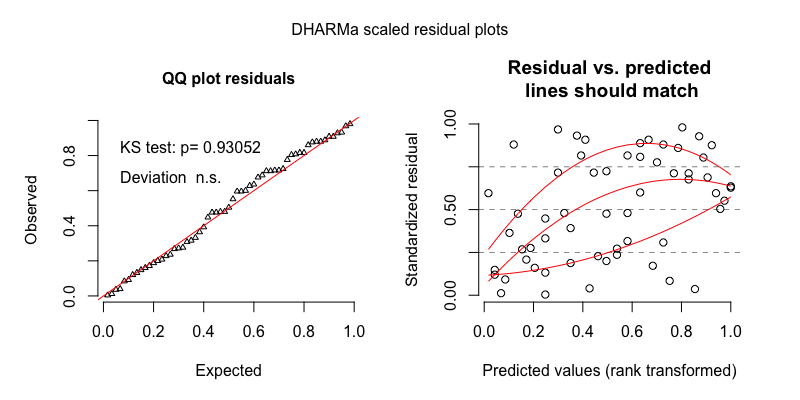
\includegraphics[width=0.9\linewidth]{www/o_c_tpm_turntaking_log_gaus_res_plot} 

}

\caption{The model residuals from the gaussian mixed-effects regression of O--TC turn transitions/min for the turn-taking sample.}\label{fig:fig24}
\end{figure}

\FloatBarrier

\subsection{Interactive sequence duration}\label{models-seqdur}

\subsubsection{Random clips}\label{models-seqdur-random}

Other-to-target-child contingent response rate (O--TC transitions/min)
in the random clips demonstrated a skewed distribution with extra cases
of zero. We therefore modeled it using a zero-inflated negative binomial
mixed-effects regression.

\FloatBarrier

\begin{figure}[H]

{\centering 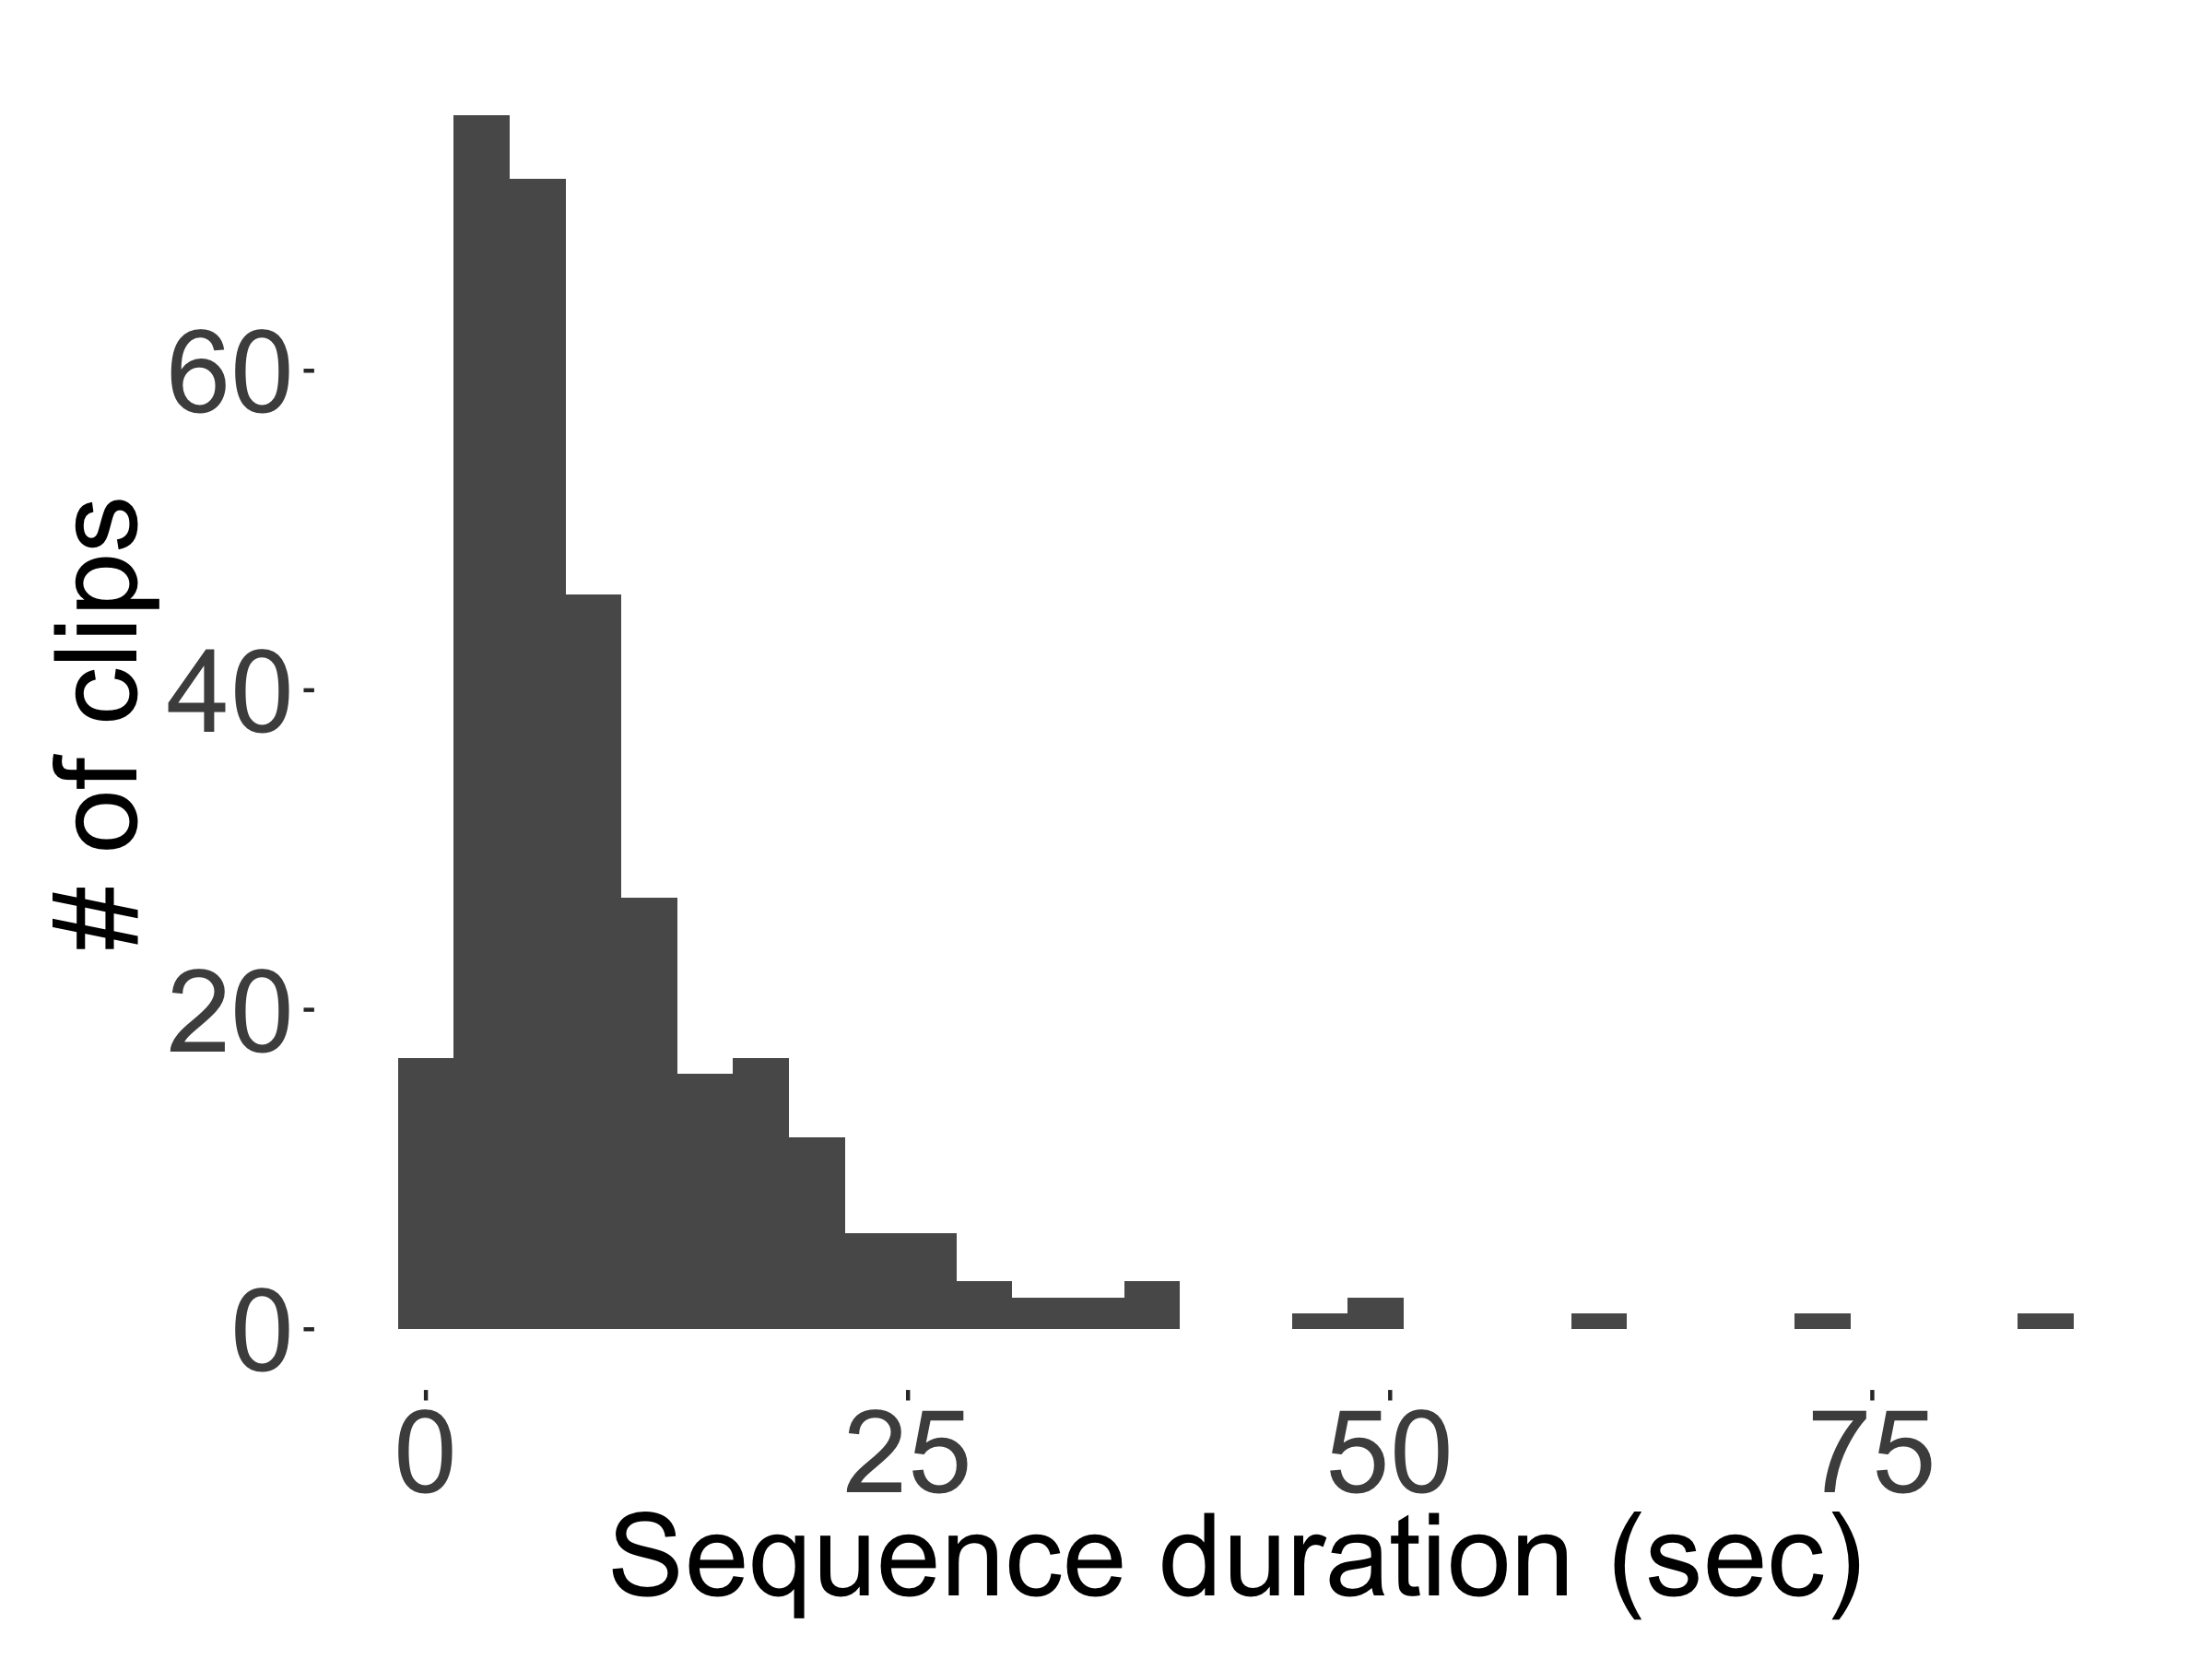
\includegraphics[width=0.4\linewidth]{www/seqdur_random_distribution} 

}

\caption{The distribution of interactive sequence duration (sec) found across the 90 random clips.}\label{fig:fig25}
\end{figure}

\FloatBarrier

\begin{table}[tbp]
\begin{center}
\begin{threeparttable}
\caption{\label{tab:tab33}Full output of the negative binomial mixed-effects regression of interactive sequence duration (sec) for the random sample, with midday as the reference level for time of day.}
\begin{tabular}{llllll}
\toprule
component & \multicolumn{1}{c}{term} & \multicolumn{1}{c}{estimate} & \multicolumn{1}{c}{std.error} & \multicolumn{1}{c}{statistic} & \multicolumn{1}{c}{p.value}\\
\midrule
cond & (Intercept) & 2.22 & 0.14 & 15.56 & 0.00\\
cond & tchiyr.std & 0.11 & 0.19 & 0.55 & 0.58\\
cond & stthr.trimorning & 0.14 & 0.17 & 0.78 & 0.44\\
cond & stthr.triafternoon & 0.13 & 0.16 & 0.80 & 0.42\\
cond & hsz.std & 0.01 & 0.08 & 0.12 & 0.90\\
cond & nsk.std & 0.01 & 0.05 & 0.13 & 0.90\\
cond & tchiyr.std:stthr.trimorning & 0.20 & 0.19 & 1.05 & 0.30\\
cond & tchiyr.std:stthr.triafternoon & 0.04 & 0.18 & 0.26 & 0.80\\
cond & tchiyr.std:hsz.std & 0.14 & 0.11 & 1.26 & 0.21\\
cond & tchiyr.std:nsk.std & -0.03 & 0.06 & -0.51 & 0.61\\
random\_effect & uniq.segment & 0.11 & NA & NA & NA\\
random\_effect & aclew\_child\_id & 0.00 & NA & NA & NA\\
\bottomrule
\end{tabular}
\end{threeparttable}
\end{center}
\end{table}

\begin{table}[tbp]
\begin{center}
\begin{threeparttable}
\caption{\label{tab:tab34}Model output of the negative binomial mixed-effects regression of interactive sequence duration (sec) for the random sample, with afternoon as the reference level for time of day.}
\begin{tabular}{llllll}
\toprule
component & \multicolumn{1}{c}{term} & \multicolumn{1}{c}{estimate} & \multicolumn{1}{c}{std.error} & \multicolumn{1}{c}{statistic} & \multicolumn{1}{c}{p.value}\\
\midrule
cond & (Intercept) & 2.35 & 0.09 & 27.16 & 0.00\\
cond & tchiyr.std & 0.15 & 0.12 & 1.26 & 0.21\\
cond & stthr.tri.amidday & -0.13 & 0.16 & -0.80 & 0.42\\
cond & stthr.tri.amorning & 0.01 & 0.12 & 0.06 & 0.95\\
cond & hsz.std & 0.01 & 0.08 & 0.12 & 0.90\\
cond & nsk.std & 0.01 & 0.05 & 0.13 & 0.90\\
cond & tchiyr.std:stthr.tri.amidday & -0.04 & 0.18 & -0.26 & 0.80\\
cond & tchiyr.std:stthr.tri.amorning & 0.15 & 0.13 & 1.17 & 0.24\\
cond & tchiyr.std:hsz.std & 0.14 & 0.11 & 1.26 & 0.21\\
cond & tchiyr.std:nsk.std & -0.03 & 0.06 & -0.51 & 0.61\\
random\_effect & uniq.segment & 0.11 & NA & NA & NA\\
random\_effect & aclew\_child\_id & 0.00 & NA & NA & NA\\
\bottomrule
\end{tabular}
\end{threeparttable}
\end{center}
\end{table}

\FloatBarrier

\begin{figure}[H]

{\centering 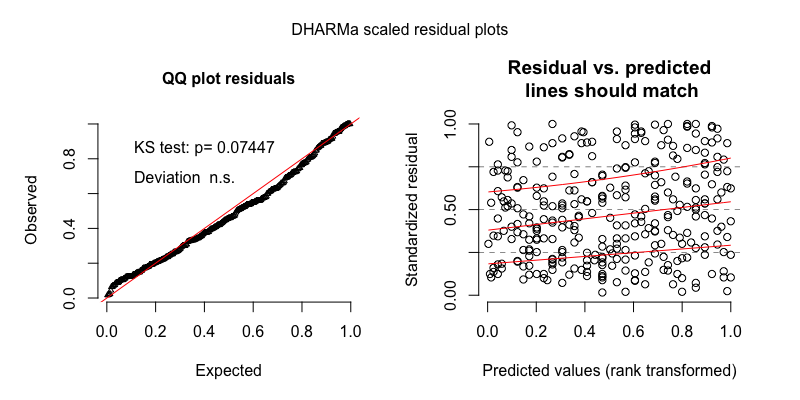
\includegraphics[width=0.9\linewidth]{www/seqdur_random_nb_res_plot} 

}

\caption{The model residuals from the negative binomial mixed-effects regression of interactive sequence duration (sec) for the random sample.}\label{fig:fig26}
\end{figure}

\FloatBarrier

\begin{table}[tbp]
\begin{center}
\begin{threeparttable}
\caption{\label{tab:tab35}Full output of the gaussian mixed-effects regression of interactive sequence duration (sec) for the random sample, with midday as the reference level for time of day.}
\begin{tabular}{llllll}
\toprule
component & \multicolumn{1}{c}{term} & \multicolumn{1}{c}{estimate} & \multicolumn{1}{c}{std.error} & \multicolumn{1}{c}{statistic} & \multicolumn{1}{c}{p.value}\\
\midrule
cond & (Intercept) & -2.24 & 0.18 & -12.46 & 0.00\\
cond & tchiyr.std & 0.10 & 0.25 & 0.41 & 0.68\\
cond & stthr.trimorning & 0.08 & 0.22 & 0.36 & 0.72\\
cond & stthr.triafternoon & 0.13 & 0.20 & 0.65 & 0.51\\
cond & hsz.std & 0.01 & 0.11 & 0.07 & 0.94\\
cond & nsk.std & 0.01 & 0.06 & 0.17 & 0.87\\
cond & tchiyr.std:stthr.trimorning & 0.34 & 0.24 & 1.39 & 0.16\\
cond & tchiyr.std:stthr.triafternoon & 0.11 & 0.22 & 0.49 & 0.62\\
cond & tchiyr.std:hsz.std & 0.17 & 0.14 & 1.15 & 0.25\\
cond & tchiyr.std:nsk.std & -0.06 & 0.08 & -0.74 & 0.46\\
random\_effect & uniq.segment & 0.19 & NA & NA & NA\\
random\_effect & aclew\_child\_id & 0.00 & NA & NA & NA\\
random\_effect & Residual & 0.85 & NA & NA & NA\\
\bottomrule
\end{tabular}
\end{threeparttable}
\end{center}
\end{table}

\begin{table}[tbp]
\begin{center}
\begin{threeparttable}
\caption{\label{tab:tab36}Model output of the gaussian mixed-effects regression of interactive sequence duration (sec) for the random sample, with afternoon as the reference level for time of day.}
\begin{tabular}{llllll}
\toprule
component & \multicolumn{1}{c}{term} & \multicolumn{1}{c}{estimate} & \multicolumn{1}{c}{std.error} & \multicolumn{1}{c}{statistic} & \multicolumn{1}{c}{p.value}\\
\midrule
cond & (Intercept) & -2.11 & 0.11 & -19.42 & 0.00\\
cond & tchiyr.std & 0.21 & 0.16 & 1.36 & 0.18\\
cond & stthr.tri.amidday & -0.13 & 0.20 & -0.65 & 0.51\\
cond & stthr.tri.amorning & -0.05 & 0.15 & -0.36 & 0.72\\
cond & hsz.std & 0.01 & 0.11 & 0.07 & 0.94\\
cond & nsk.std & 0.01 & 0.06 & 0.17 & 0.87\\
cond & tchiyr.std:stthr.tri.amidday & -0.11 & 0.22 & -0.49 & 0.62\\
cond & tchiyr.std:stthr.tri.amorning & 0.22 & 0.17 & 1.34 & 0.18\\
cond & tchiyr.std:hsz.std & 0.17 & 0.14 & 1.15 & 0.25\\
cond & tchiyr.std:nsk.std & -0.06 & 0.08 & -0.74 & 0.46\\
random\_effect & uniq.segment & 0.19 & NA & NA & NA\\
random\_effect & aclew\_child\_id & 0.00 & NA & NA & NA\\
random\_effect & Residual & 0.85 & NA & NA & NA\\
\bottomrule
\end{tabular}
\end{threeparttable}
\end{center}
\end{table}

\FloatBarrier

\begin{figure}[H]

{\centering 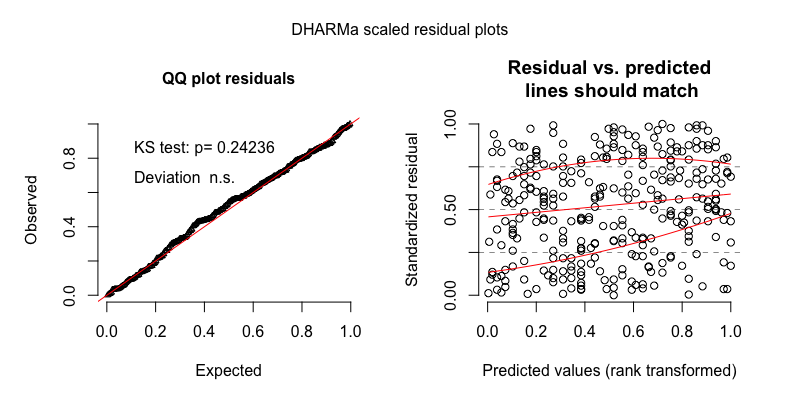
\includegraphics[width=0.9\linewidth]{www/seqdur_random_log_gaus_res_plot} 

}

\caption{The model residuals from the gaussian mixed-effects regression of interactive sequence duration (sec) for the random sample.}\label{fig:fig27}
\end{figure}

\FloatBarrier

\subsubsection{Turn-taking clips}\label{models-seqdur-turntaking}

O--TC transitions/min in the random clips demonstrated a fairly normal
distribution. We therefore modeled it using a plain (i.e.,
non-zero-inflated) negative binomial mixed-effects regression.

\FloatBarrier

\begin{figure}[H]

{\centering 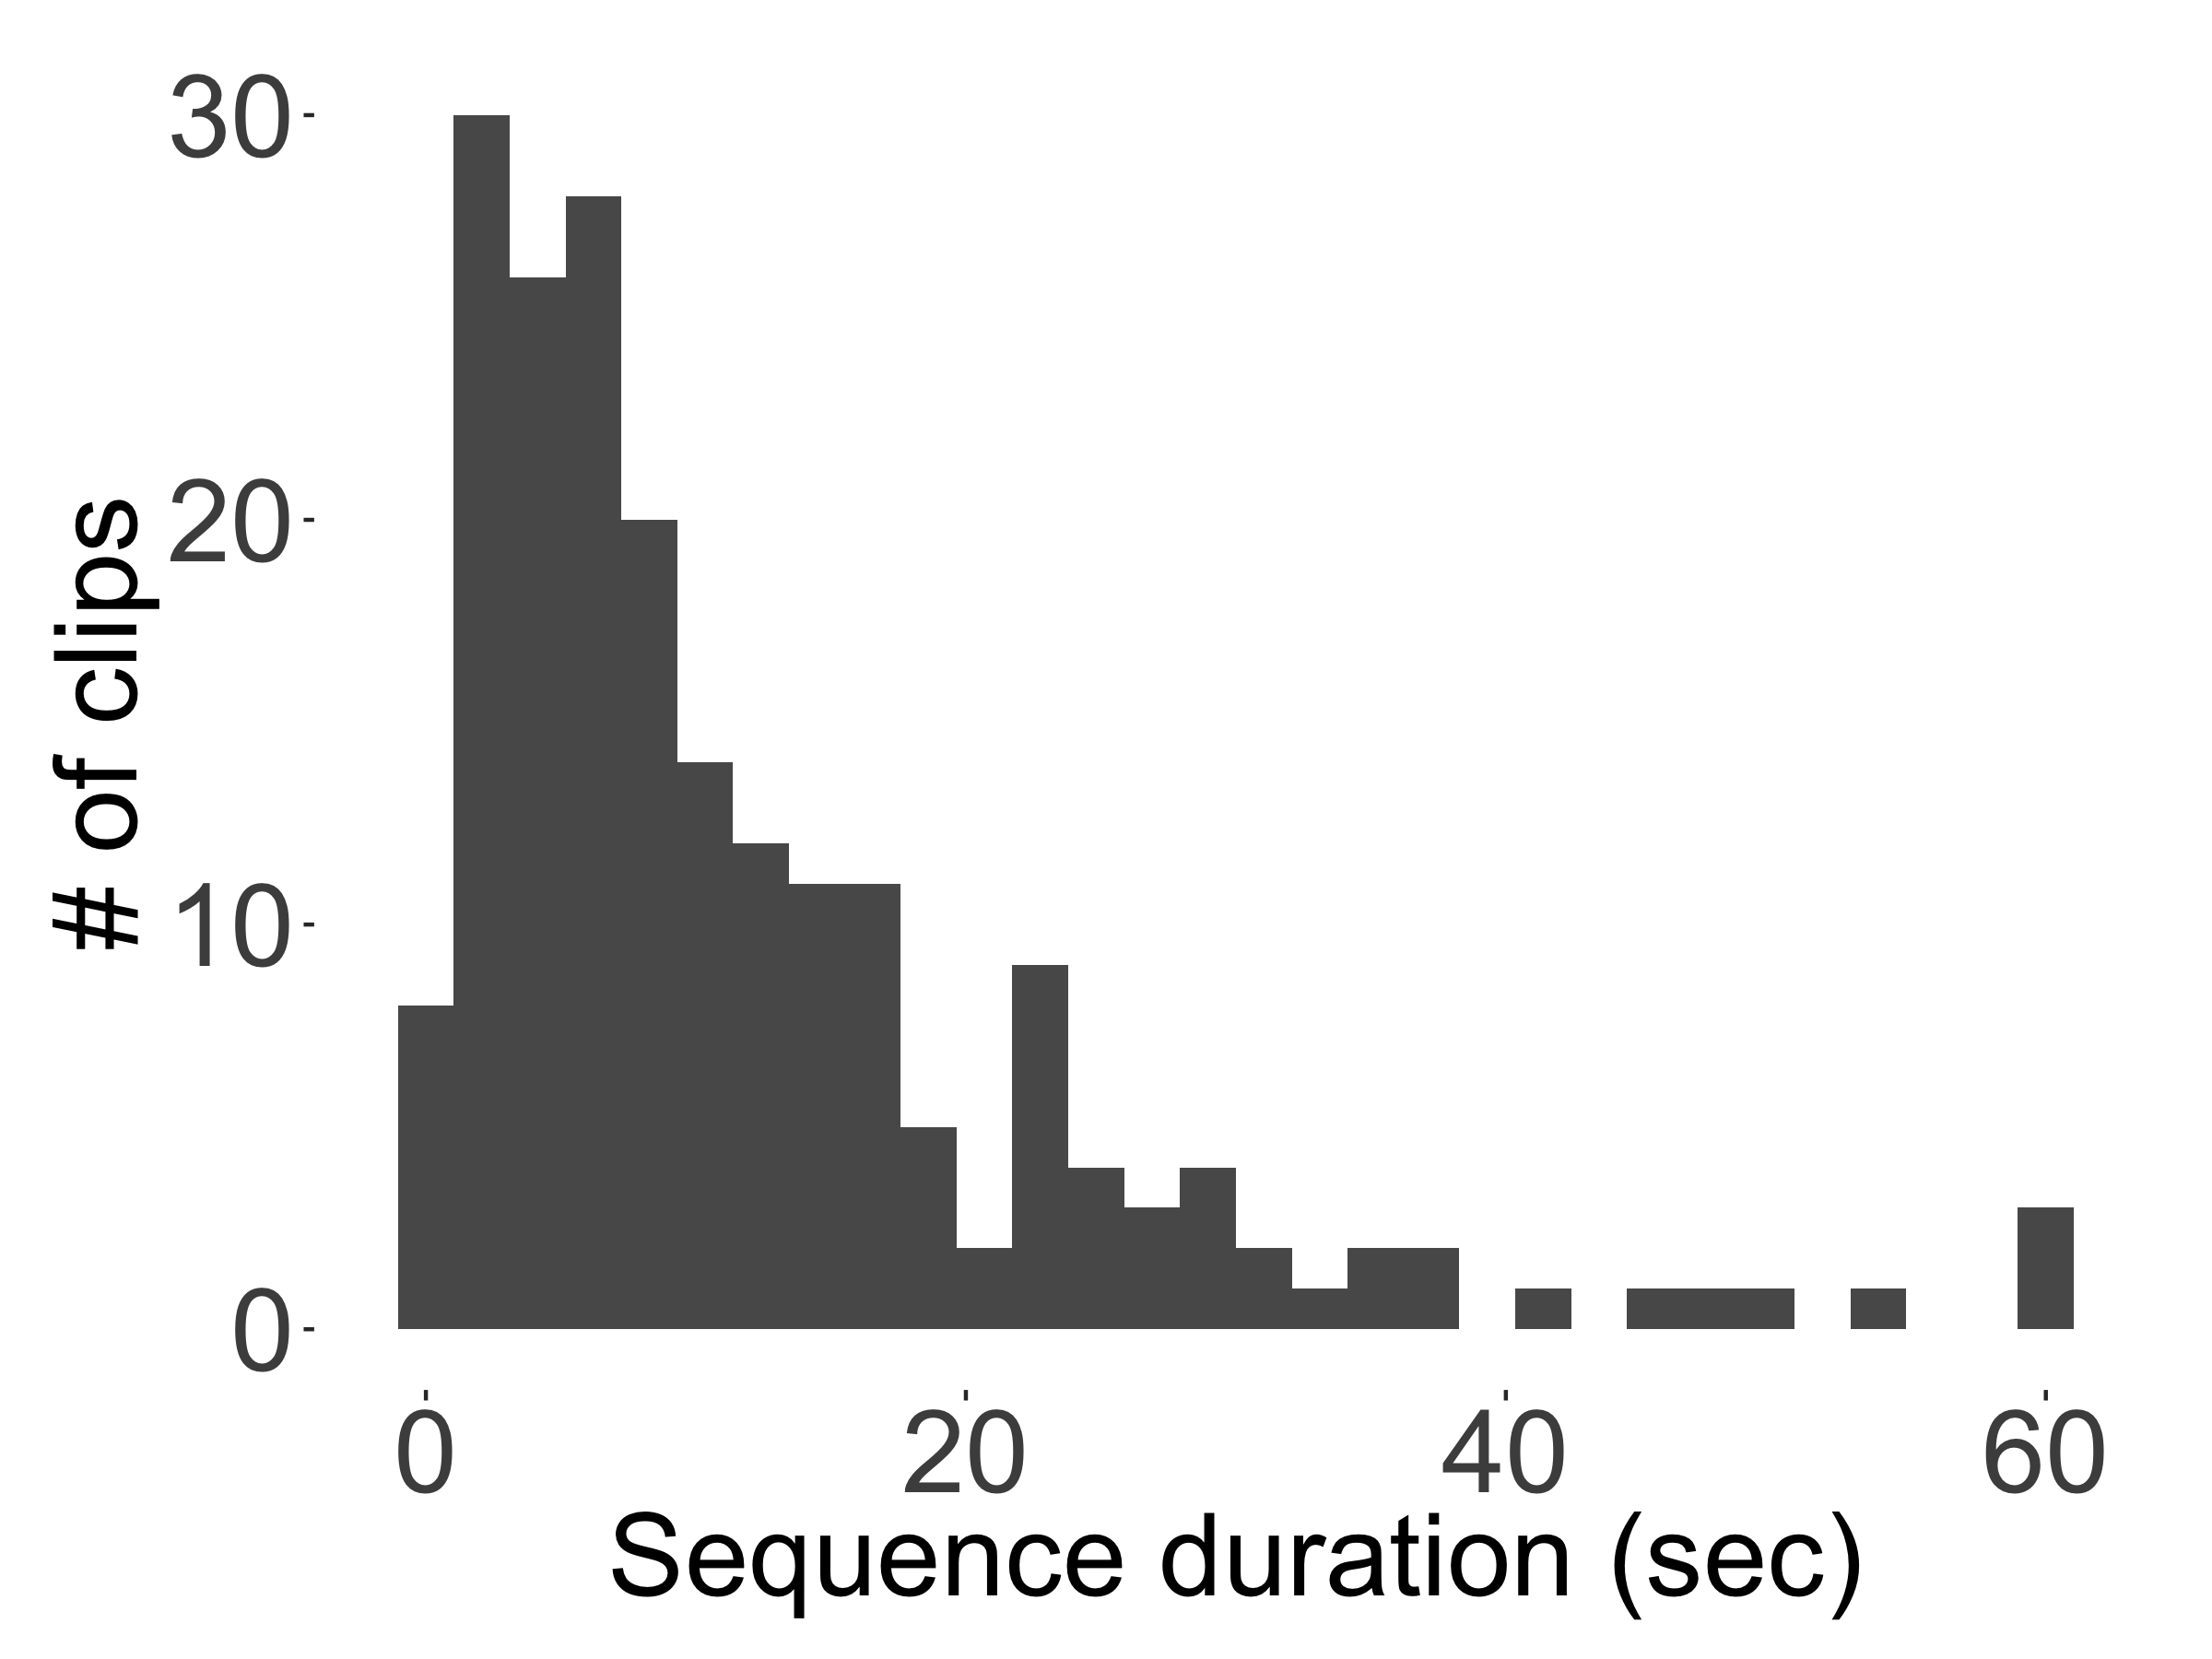
\includegraphics[width=0.4\linewidth]{www/seqdur_turntaking_distribution} 

}

\caption{The distribution of interactive sequence duration (sec) found across the 90 turn-taking clips.}\label{fig:fig28}
\end{figure}

\FloatBarrier

\begin{table}[tbp]
\begin{center}
\begin{threeparttable}
\caption{\label{tab:tab37}Full output of the negative binomial mixed-effects regression of interactive sequence duration (sec) for the turn-taking sample.}
\begin{tabular}{llllll}
\toprule
component & \multicolumn{1}{c}{term} & \multicolumn{1}{c}{estimate} & \multicolumn{1}{c}{std.error} & \multicolumn{1}{c}{statistic} & \multicolumn{1}{c}{p.value}\\
\midrule
cond & (Intercept) & 2.25 & 0.14 & 16.54 & 0.00\\
cond & tchiyr.std & -0.18 & 0.12 & -1.51 & 0.13\\
cond & stthr.trimorning & 0.06 & 0.16 & 0.37 & 0.71\\
cond & stthr.triafternoon & 0.38 & 0.14 & 2.61 & 0.01\\
cond & hsz.std & -0.17 & 0.10 & -1.74 & 0.08\\
cond & nsk.std & -0.01 & 0.06 & -0.18 & 0.85\\
cond & tchiyr.std:stthr.trimorning & -0.02 & 0.17 & -0.12 & 0.90\\
cond & tchiyr.std:stthr.triafternoon & 0.02 & 0.14 & 0.14 & 0.89\\
cond & tchiyr.std:hsz.std & -0.18 & 0.13 & -1.37 & 0.17\\
cond & tchiyr.std:nsk.std & 0.03 & 0.08 & 0.38 & 0.70\\
random\_effect & uniq.segment & 0.00 & NA & NA & NA\\
random\_effect & aclew\_child\_id & 0.00 & NA & NA & NA\\
\bottomrule
\end{tabular}
\end{threeparttable}
\end{center}
\end{table}

\begin{table}[tbp]
\begin{center}
\begin{threeparttable}
\caption{\label{tab:tab38}Model output of the negative binomial mixed-effects regression of interactive sequence duration (sec) for the turn-taking sample, with afternoon as the reference level for time of day.}
\begin{tabular}{llllll}
\toprule
component & \multicolumn{1}{c}{term} & \multicolumn{1}{c}{estimate} & \multicolumn{1}{c}{std.error} & \multicolumn{1}{c}{statistic} & \multicolumn{1}{c}{p.value}\\
\midrule
cond & (Intercept) & 2.63 & 0.12 & 20.93 & 0.00\\
cond & tchiyr.std & -0.16 & 0.13 & -1.23 & 0.22\\
cond & stthr.tri.amidday & -0.38 & 0.14 & -2.61 & 0.01\\
cond & stthr.tri.amorning & -0.32 & 0.15 & -2.12 & 0.03\\
cond & hsz.std & -0.17 & 0.10 & -1.74 & 0.08\\
cond & nsk.std & -0.01 & 0.06 & -0.18 & 0.85\\
cond & tchiyr.std:stthr.tri.amidday & -0.02 & 0.14 & -0.14 & 0.89\\
cond & tchiyr.std:stthr.tri.amorning & -0.04 & 0.17 & -0.24 & 0.81\\
cond & tchiyr.std:hsz.std & -0.18 & 0.13 & -1.37 & 0.17\\
cond & tchiyr.std:nsk.std & 0.03 & 0.08 & 0.38 & 0.70\\
random\_effect & uniq.segment & 0.00 & NA & NA & NA\\
random\_effect & aclew\_child\_id & 0.00 & NA & NA & NA\\
\bottomrule
\end{tabular}
\end{threeparttable}
\end{center}
\end{table}

\FloatBarrier

\begin{figure}[H]

{\centering 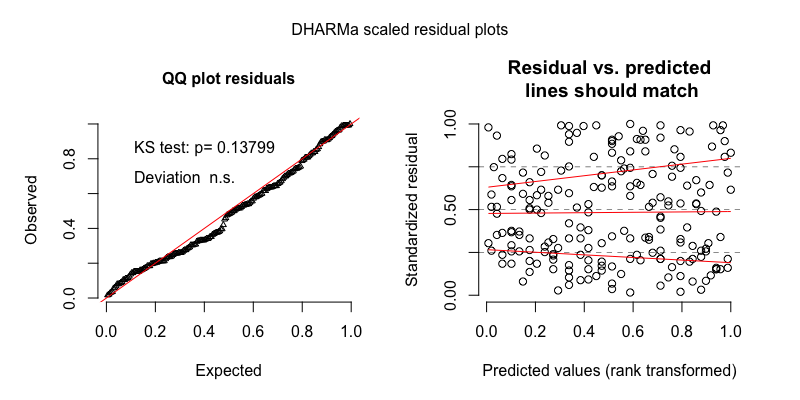
\includegraphics[width=0.9\linewidth]{www/seqdur_turntaking_nb_res_plot} 

}

\caption{The model residuals from the negative binomial mixed-effects regression of interactive sequence duration (sec) for the turn-taking sample.}\label{fig:fig29}
\end{figure}

\FloatBarrier

\begin{table}[tbp]
\begin{center}
\begin{threeparttable}
\caption{\label{tab:tab39}Full output of the gaussian mixed-effects regression of interactive sequence duration (sec) for the turn-taking sample, with midday as the reference level for time of day.}
\begin{tabular}{llllll}
\toprule
component & \multicolumn{1}{c}{term} & \multicolumn{1}{c}{estimate} & \multicolumn{1}{c}{std.error} & \multicolumn{1}{c}{statistic} & \multicolumn{1}{c}{p.value}\\
\midrule
cond & (Intercept) & -2.33 & 0.16 & -14.96 & 0.00\\
cond & tchiyr.std & -0.20 & 0.14 & -1.40 & 0.16\\
cond & stthr.trimorning & 0.08 & 0.19 & 0.39 & 0.70\\
cond & stthr.triafternoon & 0.57 & 0.18 & 3.11 & 0.00\\
cond & hsz.std & -0.23 & 0.12 & -2.01 & 0.04\\
cond & nsk.std & -0.02 & 0.07 & -0.32 & 0.75\\
cond & tchiyr.std:stthr.trimorning & 0.02 & 0.20 & 0.08 & 0.94\\
cond & tchiyr.std:stthr.triafternoon & -0.01 & 0.19 & -0.08 & 0.94\\
cond & tchiyr.std:hsz.std & -0.20 & 0.15 & -1.32 & 0.19\\
cond & tchiyr.std:nsk.std & 0.05 & 0.10 & 0.49 & 0.62\\
random\_effect & uniq.segment & 0.00 & NA & NA & NA\\
random\_effect & aclew\_child\_id & 0.00 & NA & NA & NA\\
random\_effect & Residual & 0.89 & NA & NA & NA\\
\bottomrule
\end{tabular}
\end{threeparttable}
\end{center}
\end{table}

\begin{table}[tbp]
\begin{center}
\begin{threeparttable}
\caption{\label{tab:tab40}Model output of the gaussian mixed-effects regression of interactive sequence duration (sec) for the turn-taking sample, with afternoon as the reference level for time of day.}
\begin{tabular}{llllll}
\toprule
component & \multicolumn{1}{c}{term} & \multicolumn{1}{c}{estimate} & \multicolumn{1}{c}{std.error} & \multicolumn{1}{c}{statistic} & \multicolumn{1}{c}{p.value}\\
\midrule
cond & (Intercept) & -1.75 & 0.16 & -11.17 & 0.00\\
cond & tchiyr.std & -0.22 & 0.17 & -1.29 & 0.20\\
cond & stthr.tri.amidday & -0.57 & 0.18 & -3.11 & 0.00\\
cond & stthr.tri.amorning & -0.50 & 0.19 & -2.58 & 0.01\\
cond & hsz.std & -0.23 & 0.12 & -2.01 & 0.04\\
cond & nsk.std & -0.02 & 0.07 & -0.32 & 0.75\\
cond & tchiyr.std:stthr.tri.amidday & 0.01 & 0.19 & 0.08 & 0.94\\
cond & tchiyr.std:stthr.tri.amorning & 0.03 & 0.21 & 0.14 & 0.89\\
cond & tchiyr.std:hsz.std & -0.20 & 0.15 & -1.32 & 0.19\\
cond & tchiyr.std:nsk.std & 0.05 & 0.10 & 0.49 & 0.62\\
random\_effect & uniq.segment & 0.00 & NA & NA & NA\\
random\_effect & aclew\_child\_id & 0.00 & NA & NA & NA\\
random\_effect & Residual & 0.89 & NA & NA & NA\\
\bottomrule
\end{tabular}
\end{threeparttable}
\end{center}
\end{table}

\FloatBarrier

\begin{figure}[H]

{\centering 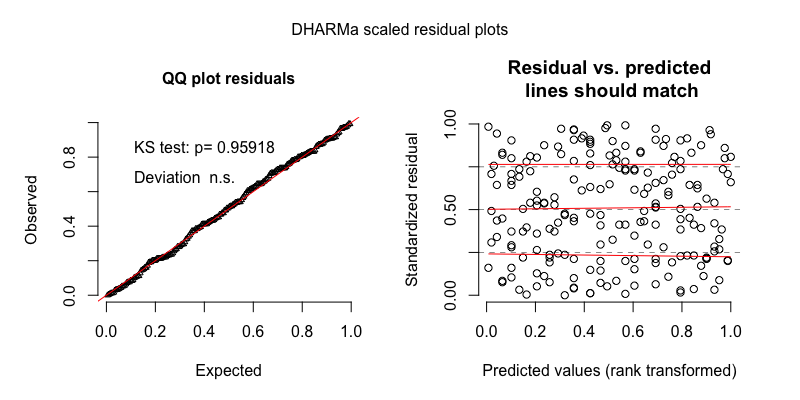
\includegraphics[width=0.9\linewidth]{www/seqdur_turntaking_log_gaus_res_plot} 

}

\caption{The model residuals from the gaussian mixed-effects regression of interactive sequence duration (sec) for the turn-taking sample.}\label{fig:fig30}
\end{figure}

\FloatBarrier

\newpage

\section{References}\label{refs}

\begingroup
\setlength{\parindent}{-0.5in} \setlength{\leftskip}{0.5in}

\hypertarget{refs}{}
\hypertarget{ref-R-glmmTMB}{}
Brooks, M. E., Kristensen, K., van Benthem, K. J., Magnusson, A., Berg,
C. W., Nielsen, A., \ldots{} Bolker, B. M. (2017a). glmmTMB balances
speed and flexibility among packages for zero-inflated generalized
linear mixed modeling. \emph{The R Journal}, \emph{9}(2), 378--400.
Retrieved from
\url{https://journal.r-project.org/archive/2017/RJ-2017-066/index.html}

\hypertarget{ref-brooks2017modeling}{}
Brooks, M. E., Kristensen, K., van Benthem, K. J., Magnusson, A., Berg,
C. W., Nielsen, A., \ldots{} Bolker, B. M. (2017b). Modeling
zero-inflated count data with glmmTMB. \emph{bioRxiv}.
doi:\href{https://doi.org/10.1101/132753}{10.1101/132753}

\endgroup






\end{document}
